% =============================================================================
%   Chapter 7: Angular Momentum Budget of the Atmosphere
%   Section 1: Angular Momentum --- Definition and Components
%
%   Lecture pages covered: pp.~2--14 (Spring 2026 lecture note)
%   Core message: 중위도 서풍은 단순한 AM 보존만으로는 설명할 수 없으며,
%                 eddy transport와 표면 토크가 결합하여 유지된다.
%                 LOD--AAM correspondence는 대기--지구가 닫힌 회전계임을 증명한다.
% =============================================================================

\section{Angular Momentum Budget}

지구 대기의 zonally averaged zonal wind $u_Z$는 위도에 따라 부호가 바뀌는
독특한 구조를 갖는다.  열대에서는 동풍(easterlies, $u_Z < 0$)이, 중위도에서는
강한 서풍(westerlies, $u_Z > 0$)이 관측되며, 이 패턴은 마찰과 다양한
표면 토크가 끊임없이 작용하고 있음에도 불구하고 계절적으로 안정적으로 유지된다.
앞 장에서 우리는 운동량(linear momentum)과 열의 자오 수송이 zonal-mean 상태를
어떻게 유지하는지 살펴보았다.  이 장에서는 \textgr{angular momentum} (각운동량,
이하 AM)이라는 회전계 고유의 보존량을 통해 같은 질문을 다시 바라본다.

회전하는 지구는 그 자체로 거대한 AM 저장소이며, 대기는 이 저장소와 끊임없이
AM을 주고받으면서 평균 상태를 유지한다.  특히 중위도 surface westerlies는 마찰에
의해 지속적으로 AM을 잃고 있으므로, 어딘가에서 AM이 공급되어야만 그 강도가
유지된다.  공급원은 열대 surface easterlies 지역이며, 이 두 위도대를 잇는
\textgr{poleward transport of AAM} (atmospheric angular momentum)이 바로
중위도 jet의 존재 자체를 설명하는 열쇠가 된다.

본 장에서는 먼저 \S1에서 AM의 정의와 두 성분 분해 ($M_\Omega + M_r$)를 다루고,
관측된 jet 강도가 단순한 AM 보존 시나리오에서 예측되는 값보다 훨씬 작다는 사실로부터
eddy momentum transport의 필요성을 도출한다.  \S2에서는 sigma 좌표계에서의 AM
보존 방정식을, \S3에서는 표면 토크(mountain torque, frictional torque, gravity wave
drag)를, \S4에서는 자오 AAM 수송을, \S5에서는 AAM의 시간 변동과 LOD와의 상관을
다룬다.

\hisu{이 장의 핵심 질문: 왜 중위도 서풍이 마찰에도 불구하고 안정적으로 유지되는가?
답은 열대로부터 중위도로의 AM 수송, 그리고 표면 토크를 통한 대기--지구 AM 교환에 있다!}

% =============================================================================
%   \subsection{Angular Momentum: Definition and Components}
% =============================================================================

\subsection{Angular Momentum: Definition and Components}

회전하는 좌표계인 지구 위에서 AM을 정의할 때 가장 흔한 오류는 지구 표면에 대한
상대 속도($\vec{V}$)로 AM을 계산해 버리는 것이다.  AM의 보존 법칙은 \emph{관성계}
(inertial frame)에서만 성립하므로, AM은 반드시 \textgr{absolute velocity}
$\vec{V}_a$를 사용하여 정의되어야 한다.  본 절에서는 절대 속도로부터 AM을 정의하고,
이를 지구 자전에 의한 부분 $M_\Omega$와 상대풍에 의한 부분 $M_r$로 분해한 뒤,
극방향으로 단열 이동하는 공기 입자의 사고 실험을 통해 AM 보존만으로 예측되는
서풍 속도가 비현실적으로 크다는 사실을 보인다.  마지막으로 hemispheric/global
적분과 LOD(length of day) 변동의 관측을 통해 대기--지구가 실제로 닫힌 AM
교환계임을 확인한다.

% --------------------------------------------------------------------------
\subsubsection{Definition of Angular Momentum}

AM의 일반적 정의는 위치 벡터와 운동량 벡터의 외적이다.  지구의 자전축과 회전각속도를
각각 $\vec{\Omega}$라 하고, 지구 중심으로부터 잰 위치 벡터를 $\vec{r}$이라 하자.
지표에 고정된 회전 좌표계에서 본 바람을 $\vec{V}$라고 하면, 절대 속도는
다음과 같이 주어진다.
\begin{equation}\label{eq:ch07_am_absvel}
  \vec{V}_a \;=\; \vec{V} \,+\, \vec{\Omega}\times\vec{r}.
\end{equation}

\begin{definition}[Angular Momentum per Unit Mass]\label{def:ch07_am_basic}
단위 질량당 각운동량 $\vec{M}$은 위치 벡터와 절대 속도의 외적으로 정의된다.
\begin{equation}\label{eq:ch07_am_def}
  \boxed{\;\vec{M} \;\equiv\; \vec{r}\times\vec{V}_a
       \;=\; \vec{r}\times\vec{V} \,+\, \vec{r}\times(\vec{\Omega}\times\vec{r}).\;}
\end{equation}
질량 $m$을 갖는 입자의 경우 전체 AM은 $m\vec{M}$이다.
\end{definition}

\hisu{AM은 반드시 절대 속도 $\vec{V}_a = \vec{V} + \vec{\Omega}\times\vec{r}$로
정의해야 한다.  지표 상대속도 $\vec{V}$만 쓰면 보존 법칙이 깨진다!}

\begin{hisublock}
왜 절대 속도가 필수인가?  Newton의 운동법칙과 그로부터 유도되는 AM 보존 법칙은
\emph{관성계}에서만 성립한다.  지구는 자전하는 비관성계이므로, 지표에서 정지한
공기 입자조차 관성계에서 보면 $\Omega R \cos\phi$의 동향 속도를 갖는다.  적도에서
이 값은 $\Omega R = 7.292\times 10^{-5} \times 6.37\times 10^6 \approx 464$ m/s에
달한다.  이 거대한 ``배경 AM''을 무시하면 어떤 AM 분석도 정량적으로 의미가 없다.
Peixoto \& Oort (1992) Ch.~11에서도 이 점을 강조하고 있다.
\end{hisublock}

\noindent
회전축 방향을 따라 분해하면 $\vec{M}$의 \emph{자전축에 평행한 성분만이} 보존 논의에서
의미를 가진다.  자전축에 수직한 성분은 지구의 강체 운동에 의해 \emph{torque-free}
회전을 그대로 따라가므로 동역학적 정보를 거의 담지 않는다.  이하에서 별다른 언급이
없으면 $M$은 자전축 평행 성분의 크기를 의미한다.

\begin{theorem}[AM Conservation for a Closed System]\label{thm:ch07_am_conservation}
대기와 고체 지구를 합친 system에 외부 토크가 무시될 수 있다면, 그 \emph{전체} AM의
시간 평균은 보존된다.
\begin{equation}\label{eq:ch07_am_cons}
  \frac{d\,\overline{M}_{\text{total}}}{dt} \;=\; 0.
\end{equation}
여기서 $\overline{(\cdot)}$는 충분히 긴 시간 평균이며, ``total''은 대기와 고체 지구를
모두 포함한 적분이다.
\end{theorem}

\hisu{대기와 고체 지구를 합친 시스템에는 외부 토크가 사실상 없으므로, 둘 사이의
AM 교환은 \emph{내부 redistribution}일 뿐 총합은 변하지 않는다.}

\begin{remark}[Where the External Torques Are]
태양 복사, 달의 조석, 우주 먼지 등이 잠재적 외부 토크의 후보이지만, 1년 이하의
스케일에서 이들은 대기--지구 내부 토크 (mountain torque, friction torque) 대비
$\sim 10^{-4}$ 이하로 작다.  따라서 한 해 미만 시간 스케일에서는
\eqref{eq:ch07_am_cons}가 매우 정확하게 성립한다.  반대로 대기만 떼어내서 보면
지표 토크가 \emph{외부 토크}로 작용하므로, 대기 단독의 AM (AAM)은 보존되지 않는다.
\end{remark}

% --------------------------------------------------------------------------
\subsubsection{Two Components: \texorpdfstring{$M_\Omega$}{M\_Omega} and \texorpdfstring{$M_r$}{M\_r}}

\eqref{eq:ch07_am_def}의 두 항을 자전축 평행 성분으로 투영하면 다음과 같이
정리된다.  지구를 반지름 $R$의 구로 근사하고, 위도 $\phi$에서 자전축까지의
수직 거리는 $R\cos\phi$이다.  지표에 대해 동향 상대풍 속도를 $u$라 하면,
절대 동향 속도는 $u + \Omega R\cos\phi$이고, 회전축 둘레의 AM은 (수직 거리) $\times$
(절대 동향 속도)로 다음과 같이 쓰여진다.
\begin{equation}\label{eq:ch07_am_components_raw}
  M \;=\; R\cos\phi \,\bigl(u + \Omega R\cos\phi\bigr)
       \;=\; \Omega R^2 \cos^2\phi \,+\, u\,R\cos\phi.
\end{equation}

\begin{definition}[Two Components of AM]\label{def:ch07_am_two}
단위 질량당 AM의 자전축 평행 성분은 다음 두 부분으로 분해된다.
\begin{equation}\label{eq:ch07_am_components}
  \boxed{\;M \;=\; M_\Omega + M_r,
   \qquad
   M_\Omega \;=\; \Omega R^2 \cos^2\phi,
   \qquad
   M_r \;=\; u\,R\cos\phi.\;}
\end{equation}
$M_\Omega$를 \textgr{$\Omega$-angular momentum} (또는 \textgr{Earth AM}),
$M_r$을 \textgr{relative angular momentum}이라 부른다.
\end{definition}

\hisu{$M_\Omega$는 ``공기가 지구와 함께 강체 회전할 때''의 AM이고, $M_r$은 그로부터의
편차, 즉 \emph{지표에서 본 바람}이 가진 AM이다.}

\begin{hisublock}
물리적 해석:
\begin{itemize}
  \item $M_\Omega = \Omega R^2 \cos^2\phi$ — 위도 $\phi$에서 정지한 공기조차 관성계에서
        보면 갖고 있는 AM.  극에서는 $\cos\phi = 0$이라 $M_\Omega = 0$, 적도에서는
        최대 ($\Omega R^2 \approx 7.292\times 10^{-5} \times (6.37\times 10^6)^2
        \approx 2.96\times 10^9$ m$^2$/s).
  \item $M_r = u R\cos\phi$ — 서풍($u>0$)이면 양, 동풍($u<0$)이면 음.  중위도 jet에서
        $u\sim 30$ m/s, $R\cos 45^\circ \approx 4.5\times 10^6$ m이므로 $M_r
        \approx 1.35\times 10^8$ m$^2$/s.  이는 같은 위도의 $M_\Omega \approx 1.48\times
        10^9$ m$^2$/s에 비해 약 10\%에 불과하다.
  \item 따라서 단위 질량으로 보면 $M_\Omega \gg M_r$이며, 후술하듯 전체 질량을
        고려하면 그 차이는 $\sim 10^6$배까지 벌어진다.
\end{itemize}
\end{hisublock}

\begin{figure}[ht]
  \centering
  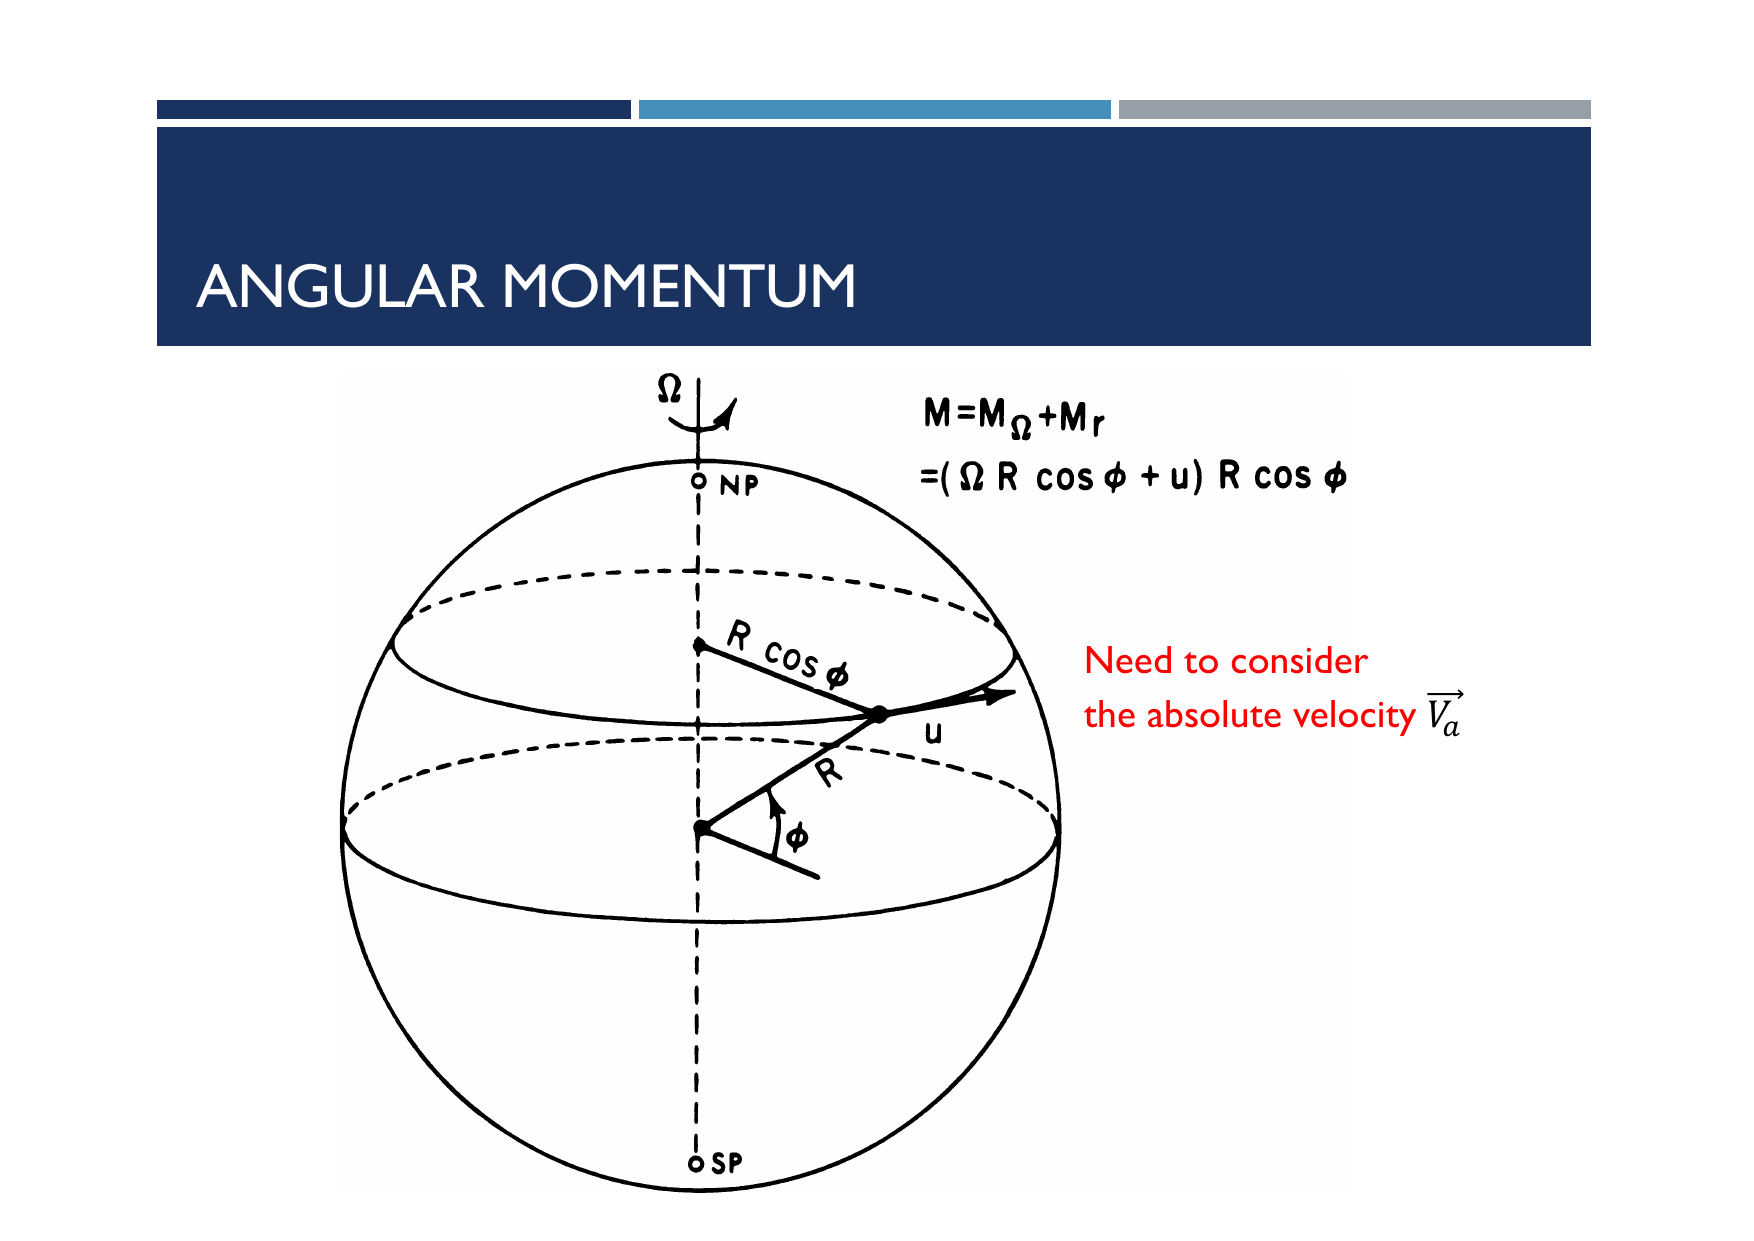
\includegraphics[width=0.85\textwidth]{images/ch07/p05_img01.png}
  \caption{Geometric construction of angular momentum on the rotating Earth.
  The position vector $\vec{r}$ from the Earth's center, the absolute velocity
  $\vec{V}_a = \vec{V}+\vec{\Omega}\times\vec{r}$, and the rotation axis are shown.
  Only the component of $\vec{r}\times\vec{V}_a$ parallel to $\vec{\Omega}$ is
  dynamically relevant for the zonal-mean AM budget; this projection involves
  $\cos\phi$, the perpendicular distance to the rotation axis is $R\cos\phi$,
  and the two contributions $M_\Omega$ (solid rotation) and $M_r$ (relative wind)
  follow naturally. \hisu{AM의 기하학적 구성도.  자전축에 평행한 성분만이 의미를
  가지며, 자전축까지의 수직 거리 $R\cos\phi$가 두 성분 분해의 핵심이다.}}
  \label{fig:ch07_am_geometry}
\end{figure}

% --------------------------------------------------------------------------
\subsubsection{Example: AM Conservation of a Polewards-Moving Parcel}

위에서 도출한 두 성분 분해를 가장 잘 보여 주는 사고 실험은 ``적도에서 정지한
공기 입자가 마찰 없이 극 방향으로 단열 이동할 때 도달 위도에서의 동향 속도가
얼마나 될 것인가?''이다.  이 예제는 두 가지 중요한 사실을 동시에 드러낸다.
첫째, 절대 속도를 사용해야만 일관된 답이 나온다는 점.  둘째, 단순 AM 보존만으로는
실제 중위도 jet 강도를 설명할 수 없다는 점.

\begin{example}[Polewards-Moving Parcel and the Necessity of Eddy
Transport]\label{ex:ch07_am_polewards}
한 공기 입자가 적도($\phi=0$)에서 지표에 대해 정지($u=0$)해 있다고 하자.  이 입자가
마찰과 토크 없이 단열적으로 위도 $\phi$까지 이동한다고 가정한다.  AM 보존을
적용하면 도달 위도에서의 동향 속도 $u(\phi)$는 얼마인가?

\textbf{Step 1 (적도에서의 AM):}
출발점에서 $u=0$이므로 $M_r = 0$이고, $M_\Omega = \Omega R^2 \cos^2 0 = \Omega R^2$.
따라서 초기 AM은
\begin{equation}\label{eq:ch07_am_ex_init}
  M_{\text{init}} \;=\; \Omega R^2.
\end{equation}

\textbf{Step 2 (위도 $\phi$에서의 AM):}
도달점에서의 AM은 \eqref{eq:ch07_am_components}로부터
\begin{equation}\label{eq:ch07_am_ex_final}
  M(\phi) \;=\; \Omega R^2 \cos^2\phi \,+\, u(\phi)\,R\cos\phi.
\end{equation}

\textbf{Step 3 (보존 조건 적용):}
$M_{\text{init}} = M(\phi)$라 놓고 풀면,
\[
  \Omega R^2 \;=\; \Omega R^2 \cos^2\phi + u(\phi)\,R\cos\phi.
\]
양변에서 $\Omega R^2 \cos^2\phi$를 빼고 $R\cos\phi$로 나누면
\begin{equation}\label{eq:ch07_am_ex_uphi}
  \boxed{\;u(\phi) \;=\; \Omega R\,\frac{1-\cos^2\phi}{\cos\phi}
                       \;=\; \Omega R\,\frac{\sin^2\phi}{\cos\phi}.\;}
\end{equation}

\textbf{Step 4 (수치 대입):}
$\Omega = 7.292\times 10^{-5}$~rad/s, $R = 6.37\times 10^6$~m을 대입하면 $\Omega R
\approx 464$~m/s이다.  대표적 위도에서의 $u(\phi)$ 값은 다음과 같다.
\begin{center}
\begin{tabular}{c|c|c}
$\phi$ & $\sin^2\phi/\cos\phi$ & $u(\phi)$ [m/s] \\\hline
$30^\circ$ & $0.289$ & $\approx 134$ \\
$45^\circ$ & $0.707$ & $\approx 328$ \\
$60^\circ$ & $1.500$ & $\approx 696$ \\
\end{tabular}
\end{center}
특히 $60^\circ$N에서 $u \approx 696$~m/s, $30^\circ$N에서 이미 $\approx 134$~m/s가
얻어지는데, 이는 관측된 중위도 jet 최대값($\sim 30$--$40$~m/s)을 \emph{한 자릿수
이상 초과}한다.

\textbf{Step 5 (결론):}
실제 대기에서는 이 입자가 도달하기도 전에 $u$가 너무 커져 dynamic instability를
일으키고, 큰 진폭의 eddy가 발생하여 \emph{역으로 AM을 적도쪽으로 운반}하거나 표면
마찰을 통해 지구에 AM을 돌려준다.  즉 ``단순 AM 보존만으로 jet를 만든다''라는
시나리오는 자기 모순적이며, \textgr{eddy momentum transport}와 표면 토크가
필수적임을 \emph{역설적으로} 증명한다.
\end{example}

\hisu{60$^\circ$N에서 700~m/s급 서풍은 관측의 20배.  ``AM만 보존되어도 jet이
만들어진다''라는 단순 논리는 깨지고, 결국 eddy가 AM을 재분배해야 jet이 현실적
강도로 유지된다.}

\begin{remark}[Hide's Theorem이 시사하는 바]
Hide (1969)는 마찰 없는 axisymmetric 순환에서 $M$이 자오방향으로 단조감소할 수
없음을 증명하였다 (\emph{Hide's theorem}).  Example~\ref{ex:ch07_am_polewards}에서
$M$이 위도에 따라 일정하게 유지되었음에도 도달 위도에서의 $u$가 비현실적으로
커진다는 사실은, axisymmetric Hadley cell만으로는 자오 AM redistribution을 책임질 수
없으며, eddy가 \emph{본질적} 역할을 함을 다시 한 번 확인시켜 준다.  자세한 내용은
Held \& Hou (1980)와 본 책 Ch.~6 \S3을 참고하라.
\end{remark}

% --------------------------------------------------------------------------
\subsubsection{Ratio of the Two Components}

$M_\Omega$와 $M_r$의 상대 크기를 정량적으로 비교해 보자.

\begin{proposition}[Ratio $M_\Omega/M_r$]\label{prop:ch07_am_ratio}
단위 질량당,
\begin{equation}\label{eq:ch07_am_ratio}
  \frac{M_\Omega}{M_r} \;=\; \frac{\Omega R^2 \cos^2\phi}{u\,R\cos\phi}
       \;=\; \frac{\Omega R \cos\phi}{u}.
\end{equation}
관측된 $|u| \lesssim 30$--$40$~m/s 범위에서, 이 비율은 위도에 따라 $0$에서
약 $46$ 사이의 값을 갖는다.  열대($\cos\phi \approx 1$, $u\sim 10$~m/s)에서
$\Omega R \cos\phi / u \approx 46$, 중위도 jet ($u\sim 30$~m/s)에서 $\approx 10$,
적도 정확히 위에서 $u\to 0$일 때 발산하지만 물리적으로 $M_r$ 자체가 0에 가까워서
의미 없다.
\end{proposition}

\hisu{단위 질량당 $M_\Omega$가 $M_r$의 수십 배.  그러나 전체 질량을 고려하면
이 비율은 $10^6$ 정도까지 커진다.}

\begin{hisublock}
왜 전체 질량 적분에서는 $10^6$가 되는가?  $M_\Omega$의 적분 $\int_V \rho M_\Omega\,dV$는
대기 전체에서 \emph{거의 같은 부호}로 합쳐지는 반면, $M_r$은 동풍대와 서풍대에서
부호가 바뀌어 큰 폭의 상쇄가 발생하기 때문이다.  결과적으로 hemispheric 또는 global
total AAM에서 $M_\Omega$의 기여는 압도적이고, $M_r$은 변동량만을 결정한다.
이것이 \S5에서 살펴볼 ``relative AAM이 변동을 주도, total AAM 평균은 $M_\Omega$가
지배''라는 관측 사실의 수학적 배경이다.
\end{hisublock}

% --------------------------------------------------------------------------
\subsubsection{Hemispheric and Global Integrals; LOD Variations}

이제 $M$을 대기 전체 질량에 대해 적분하여 \textgr{atmospheric angular momentum}
(AAM)을 정의하자.  대기 전체 또는 반구별 AAM은 다음과 같이 쓰여진다.
\begin{equation}\label{eq:ch07_am_AAM_def}
  \text{AAM} \;\equiv\; \int_V \rho\,M\,dV
   \;=\; \int_V \rho\,(M_\Omega + M_r)\,dV.
\end{equation}
관측에 기반한 Peixoto \& Oort (1992) 식의 정량적 결과를 표~\ref{tab:ch07_am_hemispheric}에
요약한다.  단위는 $10^{25}$~kg~m$^2$/s이며, NH, SH, Global 각각에 대해 연평균 (Year),
북반구 겨울(DJF), 남반구 겨울(JJA) 값을 기재했다.

\begin{table}[ht]
  \centering
  \begin{tabular}{l|ccc}
    \hline
     & Year & DJF & JJA \\\hline
    Northern Hemisphere (NH) & $7.4$ & $9.1$ & $5.7$ \\
    Southern Hemisphere (SH) & $7.4$ & $5.8$ & $9.0$ \\
    Global                    & $14.8$ & $14.9$ & $14.7$ \\\hline
  \end{tabular}
  \caption{Hemispheric and global atmospheric angular momentum (units:
  $10^{25}$ kg m$^2$ s$^{-1}$). \hisu{반구별로는 ``겨울 반구의 AAM이 크다''는 강한
  계절성이 보이지만, 글로벌 합산값은 거의 일정함에 주목.  이는 NH와 SH가 자오
  방향으로 AM을 주고받음을 시사한다.}}
  \label{tab:ch07_am_hemispheric}
\end{table}

\begin{hisublock}
Peixoto \& Oort (1992) Table~11.1의 hemispheric AAM 값이 본 표의 수치와 일치한다.
세 가지 핵심 관찰:
\begin{enumerate}
  \item 겨울 반구의 AAM이 여름 반구보다 크다 (NH는 DJF, SH는 JJA에서 최대).
        이는 winter jet이 강하고 서풍대 폭이 넓기 때문이다.
  \item 글로벌 AAM의 계절 변동은 hemispheric 변동의 약 1/10 수준.  이는
        반구간 AM 수송이 효율적임을 의미한다.
  \item Year 평균에서 NH와 SH가 거의 같은 값을 갖는 것은 ($\approx 7.4$),
        장기 평균적으로 두 반구가 평형 상태에 있음을 보여준다.
\end{enumerate}
\end{hisublock}

\noindent
대기 AAM의 시간 변동은 직접 측정하기 어렵지만, \textgr{length of day} (LOD)의 변동을
통해 \emph{독립적으로} 추정할 수 있다.  대기와 고체 지구의 합산 AM이 보존된다는
이론~\ref{thm:ch07_am_conservation}에 따르면, 대기 AAM이 증가하면 정확히 그만큼
고체 지구 AM이 감소해야 하고, 따라서 지구 자전이 약간 느려져 LOD가 늘어난다.

\begin{equation}\label{eq:ch07_am_LOD_link}
  \Delta\,\text{LOD} \;\propto\; +\,\Delta\,\text{AAM}.
\end{equation}

\begin{figure}[ht]
  \centering
  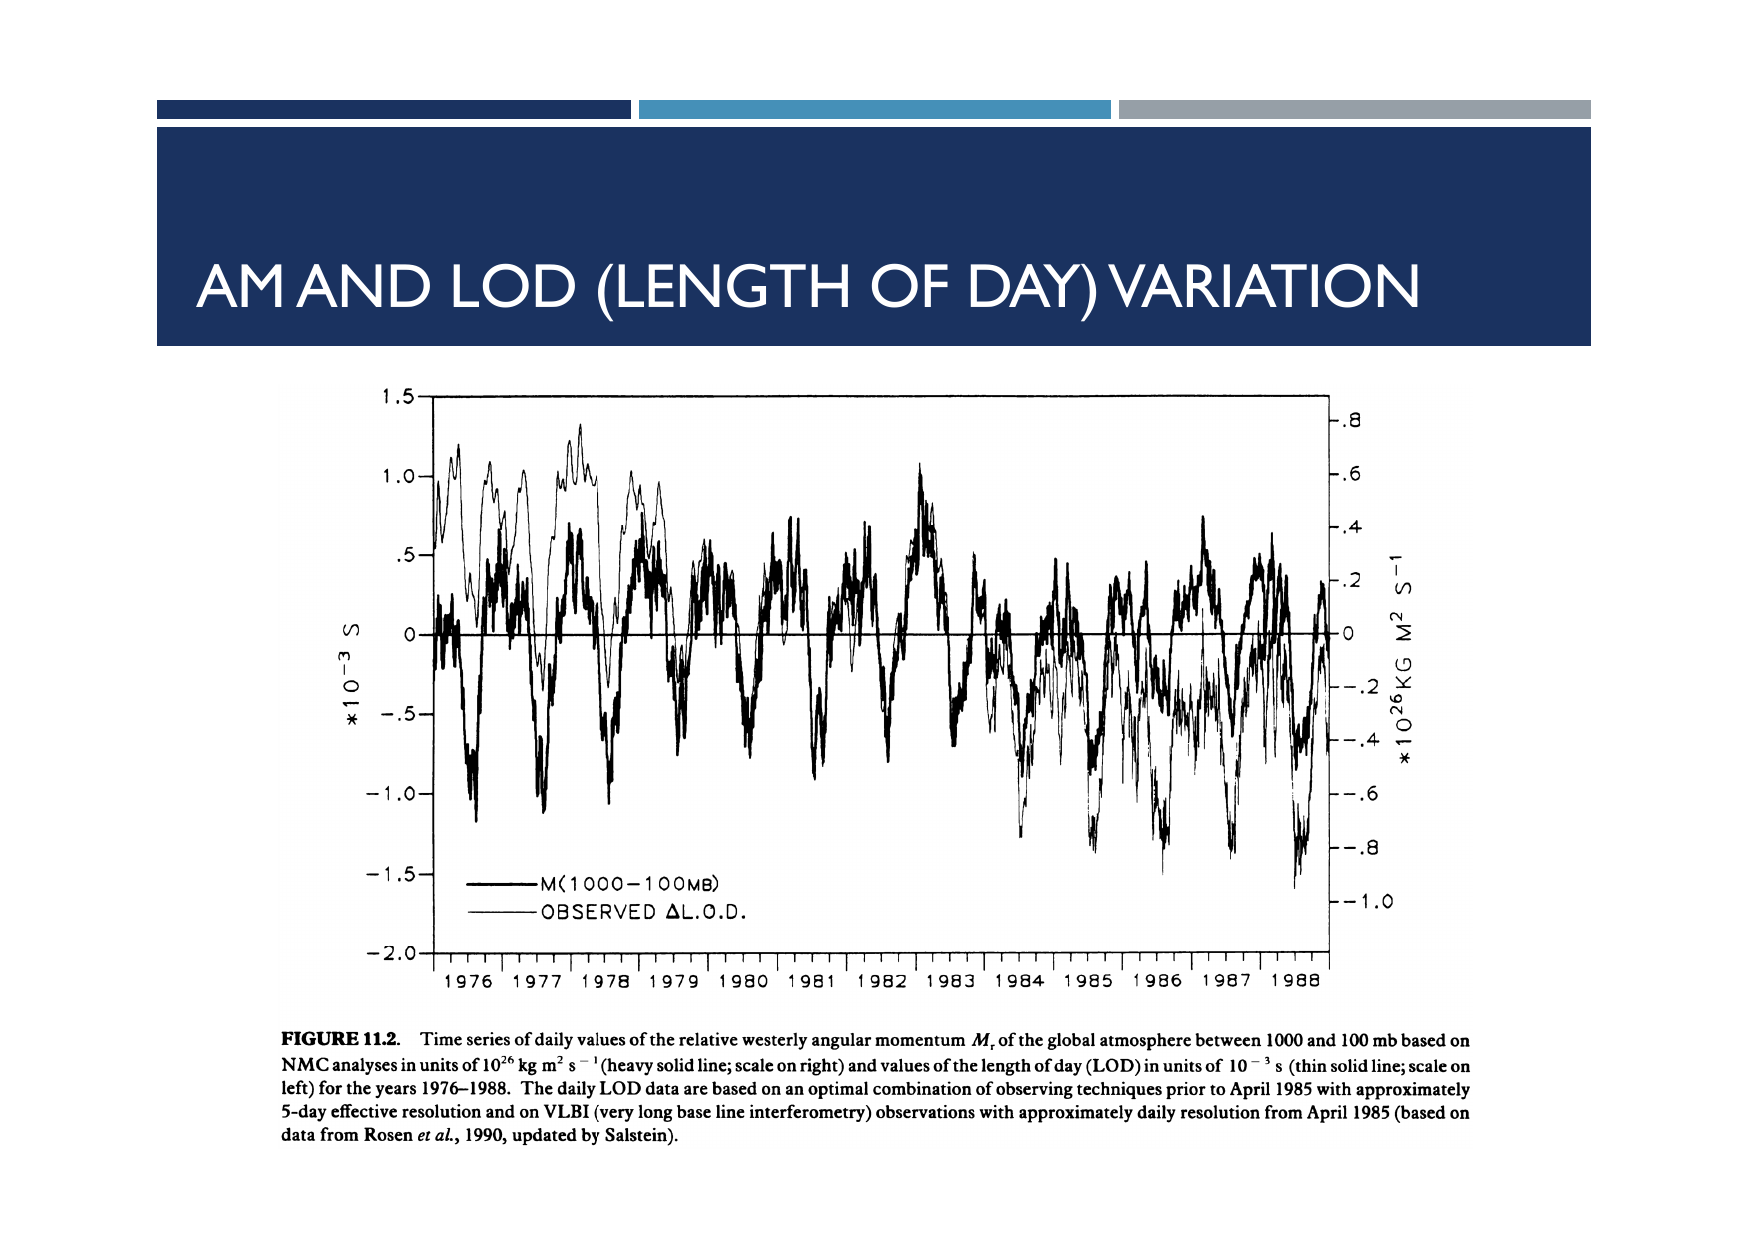
\includegraphics[width=0.85\textwidth]{images/ch07/p13_img01.png}
  \caption{Time series of atmospheric relative angular momentum $M_r$ vertically
  integrated between 1000 and 100 hPa (red, after Rosen \& Salstein) and observed
  length-of-day (LOD) anomaly (black) from 1976 to 1988.  The two curves track
  each other on time scales from intraseasonal to interannual with remarkable
  fidelity, including the strong El~Ni\~no--related peaks of 1982--83 and
  1986--87.  This near-perfect correspondence is direct observational evidence
  that the atmosphere--solid Earth pair behaves as a closed angular momentum
  system. \hisu{1976--1988년 대기 상대 AAM(빨강)과 LOD 변동(검정)은 거의 완벽히
  동기화되어 있다.  이는 대기--지구가 닫힌 AM 교환계임을 보여주는 결정적 관측
  증거이며, 1982--83 El~Ni\~no 시기 두 신호의 강한 양의 극대값이 특히
  인상적이다.}}
  \label{fig:ch07_am_lod}
\end{figure}

\begin{remark}[Closed-System Evidence]
Figure~\ref{fig:ch07_am_lod}이 갖는 함의는 매우 깊다.  AAM은 \emph{위도-고도
바람장으로부터} 계산된 값이고, LOD는 \emph{매우 정확한 천문 관측}(VLBI, lunar
laser ranging)에서 얻은 값이다.  두 수치가 완전히 독립적인 출처에서 나왔음에도
정확히 같은 패턴으로 변동한다는 것은 다음을 의미한다.
\begin{enumerate}
  \item 풍 관측으로부터 추정한 AAM은 quantitatively 신뢰할 만하다.
  \item 외부 토크(달, 태양)에 의한 LOD 변동은 1년 이하 시간 스케일에서 무시할 만하다.
  \item 따라서 대기--지구는 \emph{닫힌 AM 교환계}로 모델링해도 좋다.
\end{enumerate}
이 관측 사실은 \S2 이후의 모든 AM budget 분석의 기초가 된다.
\end{remark}

\hisu{AAM과 LOD가 같은 모양으로 변동한다 = 대기와 지구가 닫힌 회전계라는 직접
증거.  이 관측이 없었다면 AM budget 분석은 ``열역학 제2법칙 없는 열역학''에 머물렀을
것이다.}

\begin{hisublock}
\textbf{\S1 요약}:
\begin{enumerate}
  \item AM은 절대 속도 $\vec{V}_a = \vec{V} + \vec{\Omega}\times\vec{r}$로 정의하며,
        자전축 평행 성분 $M = \Omega R^2 \cos^2\phi + uR\cos\phi$의 두 항으로
        분해된다.
  \item Solid rotation 성분 $M_\Omega$가 단위 질량당 상대풍 성분 $M_r$의 수십 배,
        전체 질량 적분 시 $\sim 10^6$배.  따라서 total AAM 평균은 $M_\Omega$가,
        변동은 $M_r$이 지배한다.
  \item 적도에서 정지한 입자가 60$^\circ$N에 도달하면 AM 보존만으로는 $u\approx 696$~m/s
        가 예측되나, 관측 jet은 $\sim 30$--$40$~m/s.  따라서 eddy momentum transport와
        표면 토크에 의한 AM 재분배가 필수적이다.
  \item 1976--88년 AAM-LOD time series가 거의 완벽히 일치 → 대기--지구는 닫힌
        AM 교환계.  이 관측 사실이 \S2 이후 모든 분석의 출발점이다.
\end{enumerate}

\medskip
\textbf{다음 절(\S2)로의 연결}: 위 \emph{개념적} 보존 법칙
$d\overline{M}_{\text{total}}/dt = 0$을 \emph{국지적} 부분미분방정식 형태로
다시 쓰고, sigma 좌표계에서의 flux-form AM 방정식을 유도한다.  이 과정에서
산악 토크와 frictional 토크가 surface boundary term으로 자연스럽게 등장한다.
\end{hisublock}
% =============================================================================
%   CHAPTER 7  --  Angular Momentum Budget
%   SECTION 2  --  Conservation in Sigma Coordinates
% =============================================================================

\subsection{Conservation in Sigma Coordinates}

\S1에서 우리는 단위 질량당 절대 각운동량
\[
  M = \Omega R^2\cos^2\phi + u R\cos\phi
  \;=\; M_\Omega + M_r,
  \qquad R \equiv a\cos\phi,
\]
와 그 두 성분의 물리적 의미를 정리했다.  이 절에서는 \emph{개별 공기 덩어리}의
$M$이 어떻게 변하는지부터 출발해, 결국 \textgr{flux form}의 보존 방정식을
$\sigma$ 좌표계에서 유도하고, 이를 동서평균(zonal average) $\&$ 연직적분
(vertical integration)하여 한 위도 띠(zonal ring)에 대한
\emph{세 항(three-term)} 수지식에 도달한다.  이 세 항이 곧
\S3 surface torques 분석의 출발점이 된다.

\hisu{핵심 질문 한 줄: \emph{왜 $\sigma$ 좌표인가, 그리고 zonal ring AAM 수지를 닫는 \textbf{세 항}은 무엇인가?}}

\begin{remarkbox}
이 절의 논리적 흐름:
\begin{enumerate}
  \item 개별 공기 parcel의 $dM/dt$ ($p$ 좌표) -- 압력 경도 + eddy stress 두 항만 source.
  \item 산악 지표면 처리를 위해 $\sigma = p/p_s$ 좌표 도입.
  \item 연속 방정식 곱셈 + chain rule로 \textbf{flux form} $\partial_t(p_s M)$ 도출.
  \item Zonal averaging 4단계 (spherical divergence $\to$ chain rule $\to$ $\Phi-RT$ 정리 $\to$ 주기성).
  \item Vertical integration ($\sigma=0$ to $1$) + 하한 BC로 \textbf{세 항} 잔존.
\end{enumerate}
\end{remarkbox}

% --------------------------------------------------------------------------
\subsubsection{The AM Equation for an Individual Air Parcel}

먼저 single parcel의 $dM/dt$를 따져보자.  $M = M_\Omega + M_r$이므로
\begin{equation}\label{eq:ch07_cons_dMdt_split}
  \frac{d M}{dt}
  \;=\;
  \frac{d M_\Omega}{dt} + \frac{d M_r}{dt}.
\end{equation}
여기서 $d/dt$는 Lagrangian 시간 미분, 즉 공기 덩어리를 따라가며 보는 변화율이다.

\medskip



\noindent\textbf{$M_\Omega$ 항의 시간 변화.}
$M_\Omega = \Omega R^2\cos^2\phi = \Omega (a\cos\phi)^2\cos^2\phi$로 정의되어 있는데,
실제로는 회전축까지의 거리 $r_\perp = R\cos\phi = a\cos^2\phi$가 위도와 함께
변할 뿐 아니라, 공기 덩어리가 수직으로 움직이면 $R$ 자체가 $a+z$로 바뀐다.
편의상 $R^2$의 변동만 추적하면 ($\cos\phi$는 위도 미분 시 별도로 등장)
\begin{equation}\label{eq:ch07_cons_dMOmega}
  \frac{d M_\Omega}{dt}
  \;=\;
  \Omega\,(\cos\phi)^2 \,\frac{d R^2}{dt}
  \;=\;
  \Omega\,(\cos\phi)^2 \cdot 2 R\,\frac{dR}{dt}
  \;=\;
  \Omega\,(\cos\phi)^2 \cdot 2 R\,w,
\end{equation}
여기서 마지막 등식은 수평 운동이 회전축 거리 $R = a+z$에 직접 영향을 주지
않는다는 근사하에서 $dR/dt \approx dz/dt = w$를 쓴 결과이다.

\hisu{지구 자전이 만드는 솔리드 회전 AM은, 공기가 위로 올라가 (회전축으로부터 멀어져) $R$이 커지면 같이 커진다.}

\medskip



\noindent\textbf{$M_r$ 항의 시간 변화.}
$M_r = u R\cos\phi$의 라그랑지 미분은
\begin{equation}\label{eq:ch07_cons_dMr_raw}
  \frac{d M_r}{dt}
  \;=\;
  R\cos\phi\,\frac{d u}{dt}
  \;+\; u\cos\phi\,\frac{d R}{dt}
  \;+\; u R\,\frac{d(\cos\phi)}{dt}.
\end{equation}
구면 좌표계의 운동 방정식(예: Holton \& Hakim Ch.~2의 $u$-방정식)에서
metric 항을 정리하면 $du/dt$에 등장하는 곡률·Coriolis 기여를 모아
\begin{equation}\label{eq:ch07_cons_dMr_clean}
  \boxed{\;
  \frac{d M_r}{dt}
  \;=\;
  v f R\cos\phi
  \;-\;
  \bar f\, w\, R\cos\phi
  \;-\; a\cos\phi\,\frac{\partial \Phi}{\partial x}
  \;-\; g\,a\cos\phi\,\frac{\partial \tau_E^x}{\partial p},
  \;}
\end{equation}
여기서
\[
  f \;\equiv\; 2\Omega\sin\phi,
  \qquad
  \bar f \;\equiv\; 2\Omega\cos\phi,
\]
이고 $\tau_E^x$는 위쪽으로의 운동량 flux (eddy stress) 부호 규약을 따른다.

\hisu{$f$는 익숙한 Coriolis 매개변수, $\bar f$는 그 \emph{수평 성분} (회전축의 적도-방향 사영). 둘이 합쳐져 전체 Coriolis가 된다.}

\medskip



\noindent\textbf{두 항의 합성 -- 솔리드 회전 부분의 상쇄.}
\eqref{eq:ch07_cons_dMOmega}와 \eqref{eq:ch07_cons_dMr_clean}을 더하면
$\bar f w R\cos\phi = 2\Omega\cos\phi \cdot w R\cos\phi = 2\Omega R w \cos^2\phi$가
정확히 \eqref{eq:ch07_cons_dMOmega}의 $\Omega(\cos\phi)^2\cdot 2Rw$와 \emph{부호
반대}로 상쇄된다.  마찬가지로 $vfR\cos\phi$ 항은 사실 솔리드 회전 부분의
위도 변화를 다시 들여다보면 $\Omega R^2 \cos^2\phi$의 $\phi$ 의존성에서 나오는
기여와 상쇄된다.

\begin{theorem}[Individual Parcel AM Equation in Pressure Coordinates]\label{thm:ch07_cons_parcel}
거시적 metric 효과와 Coriolis가 정확히 상쇄된 뒤, 단위 질량 공기 덩어리
$M = \Omega R^2\cos^2\phi + u R\cos\phi$의 라그랑지 변화율은 \emph{오직} 다음
두 source에 의해서만 결정된다.
\begin{equation}\label{eq:ch07_cons_parcel}
  \boxed{\;
  \frac{d M}{dt}
  \;=\;
  -\, a\cos\phi
  \left[\,
    \frac{\partial \Phi}{\partial x}
    \;+\;
    g\,\frac{\partial \tau_E^x}{\partial p}
  \,\right].
  \;}
\end{equation}
즉 (i) 동서 압력 경도 $\partial\Phi/\partial x$와 (ii) 수직 eddy stress
divergence $g\,\partial\tau_E^x/\partial p$가 \emph{유일한} AM source이다.
\end{theorem}

\begin{hisublock}
정리 \ref{thm:ch07_cons_parcel}의 물리적 의미:
\begin{itemize}
  \item Coriolis force는 \emph{내부 힘}이라 전체 시스템(공기+지구)의 AM을 바꾸지
        못한다.  그래서 \eqref{eq:ch07_cons_parcel}에는 $f v$가 보이지 않는다.
  \item 단 두 가지 외부 source만 남는다: 압력 경도 $-a\cos\phi\,\partial_x\Phi$,
        그리고 수직 운동량 flux divergence $-g a\cos\phi\,\partial_p \tau_E^x$
        (즉 \textgr{vertical eddy stress}).
  \item 지표에 닿으면 후자가 곧 \emph{frictional torque}가 되고, 산악 지형이
        있으면 전자가 곧 \emph{mountain torque}가 된다.
\end{itemize}
이 두 source가 어떻게 zonal ring 수지에서 등장하는지가 \S2.5의 결론, 그리고 \S3
전체의 주제이다.
\end{hisublock}

% --------------------------------------------------------------------------
\subsubsection{Why Sigma Coordinates?}

\eqref{eq:ch07_cons_parcel}은 \emph{등압면(isobaric, $p$) 좌표}에서 유도한
것이다.  하지만 zonal-mean 통합으로 가는 순간, 지표 근처에서 큰 문제가 생긴다.

\begin{definition}[Sigma Coordinate]\label{def:ch07_cons_sigma}
대기 정역학에서 \textgr{sigma coordinate}는
\begin{equation}\label{eq:ch07_cons_sigma_def}
  \sigma \;\equiv\; \frac{p}{p_s(x,y,t)},
  \qquad
  \sigma \in [0,\,1],
\end{equation}
로 정의된다.  여기서 $p_s(x,y,t)$는 시간·수평위치에 따라 변하는 표면 기압이다.
\end{definition}

\hisu{$\sigma = 0$은 대기 상한(true vacuum), $\sigma = 1$은 \emph{어디에서나} 지표.  울퉁불퉁한 산이든 평평한 바다든 $\sigma=1$이라는 한 좌표면이다.}

\begin{remark}[Why Not Isobaric?]\label{rem:ch07_cons_why_sigma}
친구에게 설명한다면 이렇게 말할 수 있다.\\
``상상해 봐, 등압면 $p = 950$\,hPa을 따라 지표를 한 바퀴 돈다고 하자.  티베트
고원 위에선 $p = 950$\,hPa이 \emph{공중}에 떠 있고, 그 아래는 산이다.  그러면
어떤 곳에선 이 면이 \emph{지하}에 있다는 황당한 결과가 나와.  그래서 산악
지형에서는 등압면이 zonal 평균에 잘 안 맞아 ($\partial/\partial x$를 통합할
때 적분 구간이 위치마다 다름)."\\
$\sigma$ 좌표는 이 문제를 \emph{좌표면을 지형에 맞춰 휘게 함으로써} 해결한다.
지표는 항상 $\sigma=1$, 대기 상단은 항상 $\sigma=0$이다.  따라서 zonal 적분
구간 $\sigma \in [0,1]$이 위치에 무관하다.
\end{remark}

\begin{hisublock}
$\sigma$ 좌표의 세 가지 핵심 이점:
\begin{enumerate}
  \item \textbf{지형 처리}: 산을 좌표면이 부드럽게 따라가 (terrain-following).
  \item \textbf{경계 조건의 단순화}: 지표면에서 \emph{질량 flux가 0}이라는
        조건이 $\dot\sigma(x,y,\sigma=1,t) = 0$이라는 단 한 줄의 식이 된다.
  \item \textbf{Zonal $\&$ vertical 적분의 일관성}: 모든 위경도에서 적분 구간이
        $[0,1]$로 같으므로, $\int_0^1 \cdots d\sigma$를 zonal mean과 자유롭게
        교환할 수 있다.
\end{enumerate}
단점: 수평 압력 경도가 \emph{두 항}으로 쪼개진다는 점 (아래 \S2.3에서 확인).
하지만 이는 \S2.4 step~2의 chain-rule로 깔끔히 정리된다.
\end{hisublock}

\medskip



\noindent\textbf{$\sigma$-좌표에서의 수직 속도.}
\[
  \dot\sigma \;\equiv\; \frac{d\sigma}{dt}
  \;=\; \frac{d}{dt}\!\left(\frac{p}{p_s}\right)
  \;=\; \frac{1}{p_s}\frac{dp}{dt} - \frac{p}{p_s^2}\frac{dp_s}{dt},
\]
가 정의된다.  \textgr{lower boundary condition}은
\begin{equation}\label{eq:ch07_cons_sigma_bc}
  \boxed{\;\dot\sigma \;=\; 0\quad\text{at}\quad \sigma = 1.\;}
\end{equation}
이는 지표면이 \emph{물질면(material surface)}이라는 사실 -- 공기는 지표를 뚫고
들어가거나 나오지 않는다 -- 을 표현한다.  대기 상단 $\sigma=0$에서도
$\dot\sigma=0$ (질량 보존)이다.

\hisu{$\sigma$ 좌표에서의 수직 BC는 단 두 줄: $\dot\sigma(\sigma=0)=0$, $\dot\sigma(\sigma=1)=0$.  이게 vertical integration이 \emph{말끔하게} 떨어지는 비결.}

\medskip



\noindent\textbf{수평 압력 경도의 분해.}
$p$-좌표의 $\partial_x \Phi|_p$와 $\sigma$-좌표의 $\partial_x \Phi|_\sigma$는
같지 않다.  Chain rule에 의해
\begin{equation}\label{eq:ch07_cons_pgrad_split}
  \left(\frac{\partial \Phi}{\partial x}\right)_p
  \;=\;
  \left(\frac{\partial \Phi}{\partial x}\right)_\sigma
  \;-\;
  \frac{\sigma}{p_s}\frac{\partial p_s}{\partial x}\,
  \frac{\partial \Phi}{\partial \sigma}.
\end{equation}
정역학($\partial\Phi/\partial p = -RT/p$, 즉 $\partial\Phi/\partial\sigma =
-RT/\sigma$)을 쓰면, $p\,\partial_x\Phi|_p = p\,\partial_x\Phi|_\sigma +
RT\,\partial_x p_s$가 된다.  이것이 다음 절에서 \emph{$p_s \partial_x\Phi +
RT\,\partial_x p_s$}라는 두 항으로 나타나는 이유다.

% --------------------------------------------------------------------------
\subsubsection{The AM Equation in Flux Form}

이제 \eqref{eq:ch07_cons_parcel}을 $\sigma$ 좌표의 flux form으로 변환한다.
출발점은 $\sigma$-좌표 연속 방정식
\begin{equation}\label{eq:ch07_cons_continuity}
  \frac{\partial p_s}{\partial t}
  \;+\;
  \nabla\!\cdot\!(p_s\,\vec V)
  \;+\;
  p_s\,\frac{\partial \dot\sigma}{\partial \sigma}
  \;=\; 0,
\end{equation}
여기서 $\vec V = (u,v)$는 수평 풍속, $\nabla\cdot$는 구면 수평 발산
연산자이다.

\medskip



\noindent\textbf{Flux form 유도 (chain rule + continuity).}
임의의 단위 질량 보존량 $\psi$에 대해 라그랑지 미분과 오일러 미분은
\[
  \frac{d \psi}{dt}
  \;=\;
  \frac{\partial \psi}{\partial t}
  \;+\;
  \vec V\!\cdot\!\nabla \psi
  \;+\;
  \dot\sigma\,\frac{\partial \psi}{\partial \sigma}.
\]
양변에 $p_s$를 곱하고, $\partial_t(p_s\psi)
= p_s\,\partial_t\psi + \psi\,\partial_t p_s$ 등 \textgr{product rule}을 이용해
정리한 뒤, \eqref{eq:ch07_cons_continuity}로 $\partial_t p_s$를 소거하면,
\begin{equation}\label{eq:ch07_cons_flux_master}
  p_s\,\frac{d \psi}{dt}
  \;=\;
  \frac{\partial}{\partial t}(p_s\psi)
  \;+\;
  \nabla\!\cdot\!(p_s\psi\vec V)
  \;+\;
  \frac{\partial}{\partial\sigma}(p_s\psi\dot\sigma).
\end{equation}

\hisu{질량가중 변수 $p_s\psi$의 \emph{flux form}.  이 식을 \emph{원료}로 $\psi \to M$만 대입하면 AM의 flux form이 즉시 나온다.}

\medskip



\noindent\textbf{$\psi = M$ 대입.}
\eqref{eq:ch07_cons_parcel}을 $p$-좌표에서 $\sigma$-좌표로 변환하면서
\eqref{eq:ch07_cons_pgrad_split}을 적용하면, source 항이 두 조각으로 갈라진다.
또한 $\partial/\partial p = (1/p_s)\partial/\partial\sigma$이므로
$g\,\partial \tau_E^x/\partial p = (g/p_s)\,\partial \tau_E^x/\partial\sigma$가 된다.
이를 \eqref{eq:ch07_cons_flux_master}에 대입하면 다음이 얻어진다.

\begin{theorem}[AM Equation in Flux Form, $\sigma$-coordinates]\label{thm:ch07_cons_fluxform}
$\sigma$-좌표에서 단위 수평 면적당 절대 각운동량 $p_s M$의 보존식은
\begin{equation}\label{eq:ch07_cons_fluxform}
  \boxed{\;
  \begin{aligned}
    \frac{\partial}{\partial t}\!\bigl(p_s M\bigr)
    \;=\;&
    -\,\nabla\!\cdot\!\bigl(p_s M \vec V\bigr)
    \;-\;
    \frac{\partial}{\partial\sigma}\!\bigl(p_s M\dot\sigma\bigr)
    \\[2pt]
    &-\,a\cos\phi\!\left[\,
        p_s\,\frac{\partial \Phi}{\partial x}
        \;+\;
        RT\,\frac{\partial p_s}{\partial x}
        \;+\;
        g\,a\cos\phi\,\frac{\partial \tau_E^x}{\partial \sigma}
      \,\right].
  \end{aligned}
  \;}
\end{equation}
\end{theorem}

\begin{hisublock}
정리 \ref{thm:ch07_cons_fluxform}의 항별 해석:
\begin{itemize}
  \item $-\nabla\!\cdot\!(p_s M\vec V)$: 수평 방향 \emph{AM flux divergence}
        (질량 가중).
  \item $-\partial_\sigma(p_s M\dot\sigma)$: 연직 방향 AM flux divergence.
  \item $-a\cos\phi\, p_s\,\partial_x\Phi$: $\sigma$-면에서 잰 동서 압력 경도.
  \item $-a\cos\phi\, RT\,\partial_x p_s$: $\sigma$-좌표로 옮길 때 생긴
        \emph{표면 기압 경도} 보정 항.  이 두 항이 \S2.4 step~2 \& 3에서
        결국 산악 토크로 \emph{합쳐진다}.
  \item $-g a^2\cos^2\phi\,\partial_\sigma \tau_E^x$: 연직 eddy stress
        divergence.  지표 BC와 만나 \emph{frictional torque}가 된다.
\end{itemize}
\end{hisublock}

\begin{remark}[Why Flux Form?]\label{rem:ch07_cons_why_flux}
Flux form \eqref{eq:ch07_cons_fluxform}은 zonal averaging과 vertical
integration에 \emph{자연스럽게} 어울린다.  발산 연산자 $\nabla\cdot$와
$\partial/\partial\sigma$ 둘 다 적분 시 표면 항(boundary term)으로 환원되기
때문이다.  Ch.~4 \S2의 maintenance equation에서도 같은 전략을 썼다
(\eqref{eq:thermo_zonal}의 zonal 평균 단계).
\end{remark}

% --------------------------------------------------------------------------
\subsubsection{Zonal Averaging -- Four Steps}

\eqref{eq:ch07_cons_fluxform}에 zonal mean $(\cdot)_Z \equiv (2\pi)^{-1}
\int_0^{2\pi}(\cdot)\,d\lambda$를 적용한다.  이 과정은 네 단계로 깔끔하게
정리된다.

\medskip



\noindent\textbf{Step 1 -- Spherical divergence를 풀어쓴다.}
$\nabla\cdot(p_s M\vec V)$를 구면 좌표에서 전개하면
\begin{equation}\label{eq:ch07_cons_step1}
  \nabla\!\cdot\!(p_s M\vec V)
  \;=\;
  \frac{1}{a\cos\phi}\frac{\partial}{\partial \lambda}\bigl(p_s M u\bigr)
  \;+\;
  \frac{1}{a\cos\phi}\frac{\partial}{\partial \phi}
    \bigl(p_s M v\cos\phi\bigr).
\end{equation}

\begin{proposition}[Vanishing of Zonal Derivatives]\label{prop:ch07_cons_zonal_vanish}
임의의 주기 함수 $a(\lambda)$ (주기 $2\pi$)에 대해,
\[
  \left(\frac{\partial a}{\partial \lambda}\right)_Z
  \;=\;
  \frac{1}{2\pi}\!\int_0^{2\pi}\!\frac{\partial a}{\partial\lambda}\,d\lambda
  \;=\;
  \frac{1}{2\pi}\bigl[a(2\pi)-a(0)\bigr]
  \;=\; 0.
\]
\end{proposition}

\hisu{이 결과 하나로 \eqref{eq:ch07_cons_step1}의 첫째 항이 사라진다.}

\medskip



\noindent\textbf{Step 2 -- 압력 경도 항을 chain rule로 정리.}
\eqref{eq:ch07_cons_fluxform}의 압력 경도 두 항
$p_s\,\partial_x\Phi + RT\,\partial_x p_s$를 정리하자.  Product rule에 의해
\begin{align}
  p_s\frac{\partial \Phi}{\partial x}
  + RT\,\frac{\partial p_s}{\partial x}
  &\;=\;
  \frac{\partial}{\partial x}\!\bigl(p_s\Phi\bigr)
  - \Phi\,\frac{\partial p_s}{\partial x}
  + RT\,\frac{\partial p_s}{\partial x}
  \nonumber\\
  &\;=\;
  \frac{\partial}{\partial x}\!\bigl(p_s\Phi\bigr)
  - (\Phi - RT)\,\frac{\partial p_s}{\partial x}
  \nonumber\\
  &\;=\;
  p_s\,\frac{\partial(\Phi - RT)}{\partial x}
  + (\Phi - RT)\,\frac{\partial p_s}{\partial x}
  - (\Phi - RT)\,\frac{\partial p_s}{\partial x}
  + \frac{\partial}{\partial x}\!\bigl(p_s RT\bigr) \;-\; p_s\,\frac{\partial(RT)}{\partial x}
  \nonumber\\
  &\;=\;
  p_s\,\frac{\partial(\Phi - RT)}{\partial x}
  \;+\;
  \frac{\partial}{\partial x}\!\bigl(p_s RT\bigr)
  \;-\; p_s\,\frac{\partial(RT)}{\partial x}.
  \label{eq:ch07_cons_step2_raw}
\end{align}
복잡해 보이지만, 결국 우리가 원하는 형태는 \emph{$\partial/\partial x$가 바깥에
있는 항}들과 \emph{$\sigma$ 미분만 남는 항}들로 갈라놓는 것이다.  핵심은
다음 step 3의 항등식이다.

\medskip



\noindent\textbf{Step 3 -- $\Phi - RT = \Phi + \sigma\,\partial\Phi/\partial\sigma$.}
정역학 평형 (hydrostatic, $\sigma$ 형태)
\[
  \frac{\partial \Phi}{\partial \sigma}
  \;=\;
  -\,\frac{RT}{\sigma}
  \quad\Longleftrightarrow\quad
  RT \;=\; -\,\sigma\,\frac{\partial \Phi}{\partial \sigma},
\]
을 이용하면
\begin{equation}\label{eq:ch07_cons_step3_identity}
  \Phi - RT
  \;=\;
  \Phi + \sigma\,\frac{\partial \Phi}{\partial \sigma}
  \;=\;
  \frac{\partial}{\partial\sigma}\!\bigl(\sigma\,\Phi\bigr).
\end{equation}

\hisu{$\Phi - RT$는 단순히 $\partial_\sigma(\sigma\Phi)$. 즉 \emph{연직 미분이} 표면에 박혀 있다 -- 이것이 다음 vertical integration에서 surface 항으로 귀결되는 비결이다.}

\medskip



\noindent\textbf{Step 4 -- 주기성으로 $\partial/\partial\lambda$ 항 제거.}
\eqref{eq:ch07_cons_step2_raw}에서 $\partial/\partial x$가 바깥에 있는 항
$\partial_x(p_s\Phi)$, $\partial_x(p_s RT)$, 그리고 $p_s\,\partial_x(RT)$ 등은
모두 zonal mean을 취하면 (proposition~\ref{prop:ch07_cons_zonal_vanish}에 의해)
사라진다. 정확히는 $\partial_x = (a\cos\phi)^{-1}\partial_\lambda$이므로 주기
적분 시 0이다.  남는 것은
\begin{equation}\label{eq:ch07_cons_step4_pgrad}
  \left(\,p_s\,\frac{\partial\Phi}{\partial x}
  + RT\,\frac{\partial p_s}{\partial x}\right)_{\!Z}
  \;=\;
  \left(p_s\,\frac{\partial}{\partial x}(\Phi-RT)\right)_{\!Z}
  + \underbrace{\left(\frac{\partial(p_s RT)}{\partial x} - p_s\frac{\partial(RT)}{\partial x}\right)_{\!Z}}_{=0 \text{ in periodic average}},
\end{equation}
즉 두 압력 경도 항이 합쳐져 \emph{$(p_s\partial_x(\Phi-RT))_Z$} 하나로 정리된다.
\eqref{eq:ch07_cons_step3_identity}을 대입하면 이는 곧
\[
  \left(p_s\,\frac{\partial}{\partial x}\!\left[\frac{\partial(\sigma\Phi)}{\partial\sigma}\right]\right)_{\!Z}
  \;=\;
  \frac{\partial}{\partial\sigma}\!\left(\,\sigma\,p_s\,\frac{\partial\Phi}{\partial x}\,\right)_{\!Z},
\]
순서 교환이 가능한 이유는 $\partial/\partial x$와 $\partial/\partial\sigma$가
\emph{독립 좌표} 위의 편미분이기 때문이다.

\begin{theorem}[Zonally-Averaged AM Equation in $\sigma$-coordinates]\label{thm:ch07_cons_zonal}
네 단계의 결과를 모으면
\begin{equation}\label{eq:ch07_cons_zonal}
  \begin{aligned}
    \frac{\partial(p_s M)_Z}{\partial t}
    \;=\;&
    -\,\frac{1}{\cos\phi}\,\frac{\partial}{\partial y}\!
       \bigl[(p_s M v)_Z\cos\phi\bigr]
    \\[2pt]
    & -\, \frac{\partial}{\partial\sigma}\!\left[
         (p_s M\dot\sigma)_Z
         \;+\; g\,a\cos\phi\,(\tau_E^x)_Z
         \;+\; a\cos\phi\,\Bigl(\sigma\,p_s\,\frac{\partial\Phi}{\partial x}\Bigr)_{\!Z}
       \right],
  \end{aligned}
\end{equation}
여기서 $\partial/\partial y \equiv (1/a)\,\partial/\partial\phi$이다.
\end{theorem}

\hisu{모든 source가 \emph{한 줄짜리 연직 미분} 안에 들어갔다. 이제 $\int_0^1 d\sigma$만 씌우면 끝!}

\begin{hisublock}
정리 \ref{thm:ch07_cons_zonal}의 구조:
\begin{itemize}
  \item 첫째 항: 자오 방향 AM flux의 \emph{수렴/발산} -- 위도 사이의 AM
        수송을 나타낸다.
  \item 둘째 줄 ($\partial/\partial\sigma$ 안의 세 항): 모두 \emph{연직 발산}
        형태로 통일됨.  순서대로 \textbf{(a)} 자체 운동에 의한 AM의 연직 수송,
        \textbf{(b)} eddy stress (마찰), \textbf{(c)} 산악(form drag) 효과.
  \item $\partial(p_s M)_Z/\partial t$를 연직적분하면 마지막 줄이 \emph{표면 값}
        만 남게 되어 -- 이것이 \S2.5의 세 항 수지로 바로 이어진다.
\end{itemize}
\end{hisublock}

% --------------------------------------------------------------------------
\subsubsection{Vertical Integration and the Final Budget}

이제 \eqref{eq:ch07_cons_zonal}의 양변을 $\sigma$에 대해 $0$부터 $1$까지
적분한다.  적분 단위 변환은 다음 관계로 통일된다.

\begin{definition}[Mass Element in $\sigma$-coordinates]\label{def:ch07_cons_mass}
정역학 평형하에서 단위 수평면적당 질량 요소는
\begin{equation}\label{eq:ch07_cons_mass}
  \rho\,dz \;=\; \frac{1}{g}\,p_s\,d\sigma,
\end{equation}
이고, 따라서 단위 수평면적 위 전체 대기 기둥의 질량은 $p_s/g$이다.
\end{definition}

\hisu{$\sigma$ 좌표에서 \emph{한 컬럼의 질량} = 표면 기압 / 중력.  단순하면서 강력한 관계.}

\begin{definition}[Surface Geopotential Height]\label{def:ch07_cons_h}
표면 위치 ($\sigma=1$)에서의 geopotential을 $\Phi_s(x,y) \equiv
\Phi(x,y,\sigma=1)$이라 하면, 표면 \emph{지형 고도(elevation)}는
\begin{equation}\label{eq:ch07_cons_h_def}
  h(x,y) \;\equiv\; \frac{1}{g}\,\Phi(x,y,\sigma=1)
  \;=\; \frac{\Phi_s}{g}.
\end{equation}
\end{definition}

\medskip



\noindent\textbf{$\sigma=1$에서의 압력 경도 항 평가.}
\eqref{eq:ch07_cons_zonal} 둘째 줄의 세 번째 항 $\bigl(\sigma p_s
\partial_x\Phi\bigr)_Z$를 $\sigma=1$에서 평가하면
\[
  \Bigl.\bigl(\sigma p_s\,\partial_x\Phi\bigr)_Z\Bigr|_{\sigma=1}
  \;=\;
  \bigl(p_s\,\partial_x\Phi_s\bigr)_Z
  \;=\;
  g\,\bigl(p_s\,\partial_x h\bigr)_Z,
\]
정의 \ref{def:ch07_cons_h}에 의해서이다.  반면 $\sigma=0$에서는
$\sigma\,p_s\partial_x\Phi = 0$이므로 적분 후 $\sigma=1$ 표면 항만 남는다.

\medskip



\noindent\textbf{$\sigma=1$에서의 stress 항.}
지표면 마찰 stress의 값은 곧 $(\tau_E^x)_Z|_{\sigma=1}$이고, $\sigma=0$
(대기 상한)에서는 $\tau_E^x = 0$이라 가정한다 (또는 위로 빠져나가는 momentum
flux를 무시).

\medskip



\noindent\textbf{$\sigma=1$에서의 vertical AM flux $\dot\sigma$.}
\eqref{eq:ch07_cons_sigma_bc}에 의해 $\dot\sigma(\sigma=1)=0$이므로
$(p_s M\dot\sigma)_Z\big|_{\sigma=1} = 0$.  $\sigma=0$에서도 마찬가지.
따라서 이 항은 vertical integration 후 \emph{완전히 사라진다}.

\medskip



\noindent\textbf{최종 vertically-integrated zonal-ring budget.}
이상의 평가를 모두 적용하면 vertical integration된 zonal-ring AM 수지가
극적으로 간단해진다.

\begin{theorem}[Three-Term Zonal-Ring AM Budget]\label{thm:ch07_cons_threeterm}
$\sigma$-좌표에서 zonal mean과 vertical integration ($0 \le \sigma \le 1$)을
취한 절대 각운동량 수지는 정확히 세 항으로 닫힌다.
\begin{equation}\label{eq:ch07_cons_threeterm}
  \boxed{\;
  \frac{\partial}{\partial t}\!\!\int_0^1\!\!(p_s M)_Z\,d\sigma
  \;=\;
  \underbrace{-\,\frac{1}{\cos\phi}\frac{\partial}{\partial y}\!\!\int_0^1\!
              (p_s M v)_Z\cos\phi\,d\sigma}_{\text{(I) Meridional flux convergence}}
  \;\underbrace{-\,a\cos\phi\,g\,(\tau_E^x)_Z\big|_{\sigma=1}}_{\text{(II) Friction torque}}
  \;\underbrace{-\,a\cos\phi\,g\,\bigl(p_s\,\partial_x h\bigr)_Z}_{\text{(III) Mountain torque}}.
  \;}
\end{equation}
($g$ 계수는 단위와 부호 규약에 따라 흡수될 수 있으며, 이후 \S3에서는
$g$를 흡수한 정의를 쓴다.)
\end{theorem}

\hisu{Ch.~7 §2의 \emph{결론}: 한 위도 띠의 AAM 변화는 오직 세 가지가 결정한다 -- (I) 자오 수송, (II) 마찰, (III) 산악.}

\begin{hisublock}
정리 \ref{thm:ch07_cons_threeterm}의 \textbf{한국어 종합 해석}:
\begin{enumerate}
  \item \textbf{(I) Meridional flux convergence} -- 이웃 위도에서 AM이 흘러
        들어오거나(수렴) 빠져나가는(발산) 효과.  $u_E v_E$ eddy momentum flux가
        주된 기여자 (\S4의 주제).
  \item \textbf{(II) Friction torque} -- 지표 마찰이 만드는 토크.  무역풍대
        (적도 0--30$^\circ$)에서는 동풍이라 마찰이 \emph{대기에 서풍 운동량
        공급}, 즉 양(+)의 toque.  중위도 서풍대에서는 반대 부호.
  \item \textbf{(III) Mountain torque} -- 산악 동·서면 기압차에 의한 토크.
        $-(p_s\,\partial_x h)_Z$가 양수이면 산이 대기에서 AM을 \emph{빼앗는다}
        (산 서쪽 high, 동쪽 low 패턴).  현실 NH 중위도 평균에서 대기→지구 AM
        교환의 \emph{약 50\%}를 이 항이 담당한다.
\end{enumerate}
\smallskip
이 세 항이 \S3 (surface torques 자세히), \S4 (poleward transport, 즉 (I) 항의
구조), \S5 (시간 변동성) 분석의 \emph{공통 출발점}이다.
\end{hisublock}

\begin{remark}[Scale and Unit Check]\label{rem:ch07_cons_units}
\eqref{eq:ch07_cons_threeterm} 각 항의 단위는 [kg\,m$^2$\,s$^{-2}$ per unit
latitude] (즉 토크 per unit length).  대표 크기:
\begin{itemize}
  \item Friction torque: 중위도에서 $\tau_E^x \sim 0.1$\,N\,m$^{-2}$,
        $a\cos\phi \sim 5\times 10^6$\,m $\Rightarrow$ $\sim 5\times 10^5$
        N\,m\,(m latitude)$^{-1}$.
  \item Mountain torque: $p_s \sim 10^5$\,Pa, $\partial_x h \sim 10^{-3}$,
        zonal mean 후 약 10\% 잔존 $\Rightarrow$ 비슷한 order $10^5$
        N\,m\,(m lat)$^{-1}$.
\end{itemize}
즉 (II)와 (III)은 \emph{동일 차수}로 경쟁하며, 어느 한쪽이 다른 한쪽을 압도
하지 않는다 -- 이 점이 \S3 mountain vs friction 분석의 출발점이다.
\end{remark}

\begin{hisublock}
\textbf{참고 문헌 가이드 (\S2 conservation \& sigma coordinates)}:
\begin{itemize}
  \item Holton \& Hakim (2012), \textit{Intro to Dynamic Meteorology} 5th ed.,
        Ch.~10.2 -- pressure-coordinate AM 방정식과 zonal mean 처리; 본문
        \eqref{eq:ch07_cons_parcel}의 출발점이며 단, 산악 처리는 본 자료의
        $\sigma$ 좌표 접근이 더 깔끔하다.
  \item Peixoto \& Oort (1992), \textit{Physics of Climate}, Ch.~11
        (pp.~340--356) -- AAM 보존식의 \emph{flux form} 유도 (Eq.~11.12--11.18)
        를 동일한 절차로 다루며, \S2.4 step~2의 chain-rule 변형이 그들의
        Eq.~11.16와 동일하다.
  \item Lorenz (1967), \textit{Nature \& Theory of the General Circulation},
        Ch.~5 -- $\sigma$ 좌표를 처음 정식으로 large-scale dynamics에 도입한
        고전.  Lower BC $\dot\sigma|_{\sigma=1}=0$의 의미를 가장 명료하게
        설명.
  \item Phillips (1957), \textit{J. Meteor.} 14, 184--185 -- $\sigma$ 좌표의
        원조 논문.  지표면 처리의 단순함이 핵심 주장.
\end{itemize}
\end{hisublock}
% =============================================================================
%   SECTION 3 — Surface Torques: Mountain, Friction, and Gravity Waves
% =============================================================================

\subsection{Surface Torques: Mountain, Friction, and Gravity Waves}

\S2의 마지막 결과 \eqref{eq:ch07_cons_threeterm}에서 우리는 zonal ring의
vertically integrated AAM budget이 세 항으로 닫힌다는 것을 보았다:
meridional flux convergence, surface stress torque, 그리고 surface pressure
(mountain) torque.  앞 두 항은 zonal mean 흐름 자체의 dynamics와 결합되어
있으므로 이를 다음 절에서 다루기로 하고, 본 절에서는 \textbf{대기와 고체
지구 사이의 AM 교환을 직접 매개하는 두 개의 표면 torque}와 이들에
관여하는 \textgr{gravity wave drag} 메커니즘을 본다.

물리적 그림은 단순하다.  대기는 무역풍대에서 동풍을 ($u<0$),
중위도 westerly 영역에서 서풍을 ($u>0$) 가진다.  지표 마찰은 두 경우 모두
\textit{지표를 통한 AM의 흐름}을 유발하지만 부호가 반대이다.  한편 산악
지형은 동서 압력차를 통해 대기와 지구를 \textit{역학적으로} 결합시킨다.
이 두 가지 mechanism이 합쳐져서 지구 회전과 대기 순환을 연결한다.

\hisu{지표 torque 두 종류: 마찰 torque와 산 (압력) torque.
두 mechanism이 합쳐져 대기와 지구 사이의 AM 교환을 완성한다.}

% --------------------------------------------------------------------------
\subsubsection{Pressure (Mountain) Torque}

\textgr{Mountain torque}는 산악 양쪽의 \textit{동서 지표 압력차}에서 비롯된다.
산이 동쪽에서 더 높은 압력, 서쪽에서 더 낮은 압력을 받으면 ($\partial p_s/\partial x > 0$
in the mountain region) 산은 동방향으로 밀리고, 그 반작용으로 대기는
서방향 AM을 잃는다.  반대로 서쪽에서 high, 동쪽에서 low이면 대기는
westerly AM을 지구에 \textit{넘긴다}.

\begin{definition}[Pressure (Mountain) Torque per Zonal Ring]\label{def:ch07_torque_mountain}
지표 고도를 $h(x,y)$, 지표 압력을 $p_s(x,y,t)$라고 할 때, vertically integrated
AAM budget에 들어가는 산악 torque는
\begin{equation}\label{eq:ch07_torque_mountain_def}
  T_M(\phi)
   \;=\;
   -\,a\cos\phi\,\Bigl(p_s\,\frac{\partial h}{\partial x}\Bigr)_Z .
\end{equation}
여기서 $(\cdot)_Z$는 zonal average, $a\cos\phi$는 회전축으로부터의
수직거리이다.  $T_M < 0$은 대기가 지구에 westerly AM을 \textit{공급}함을,
$T_M > 0$은 그 반대를 뜻한다.
\end{definition}

\hisu{$-a\cos\phi(p_s\,\partial h/\partial x)_Z$ 부호 규약: 음수면 대기 → 지구,
양수면 지구 → 대기로 AM이 흐른다.}

\begin{remark}[Airfoil Form Drag Analogy]\label{rem:ch07_torque_airfoil}
\eqref{eq:ch07_torque_mountain_def}의 해석은 비행기 날개의 form drag와
완벽히 같은 구조이다.  westerly가 산을 만나면 산 \textbf{서쪽} (upwind)에
높은 압력이 쌓이고, \textbf{동쪽} (downwind)에 낮은 압력이 형성된다 (Bernoulli +
mountain wave 효과).  이 압력 분포가 정지된 산을 동쪽으로 미는 net force를
만든다 — 그러나 산은 움직이지 못하므로 reaction으로 대기가 서방향 (즉 westerly)
AM을 잃는다.  이것이 \textgr{form drag}이다.
\end{remark}

\begin{figure}[ht]
  \centering
  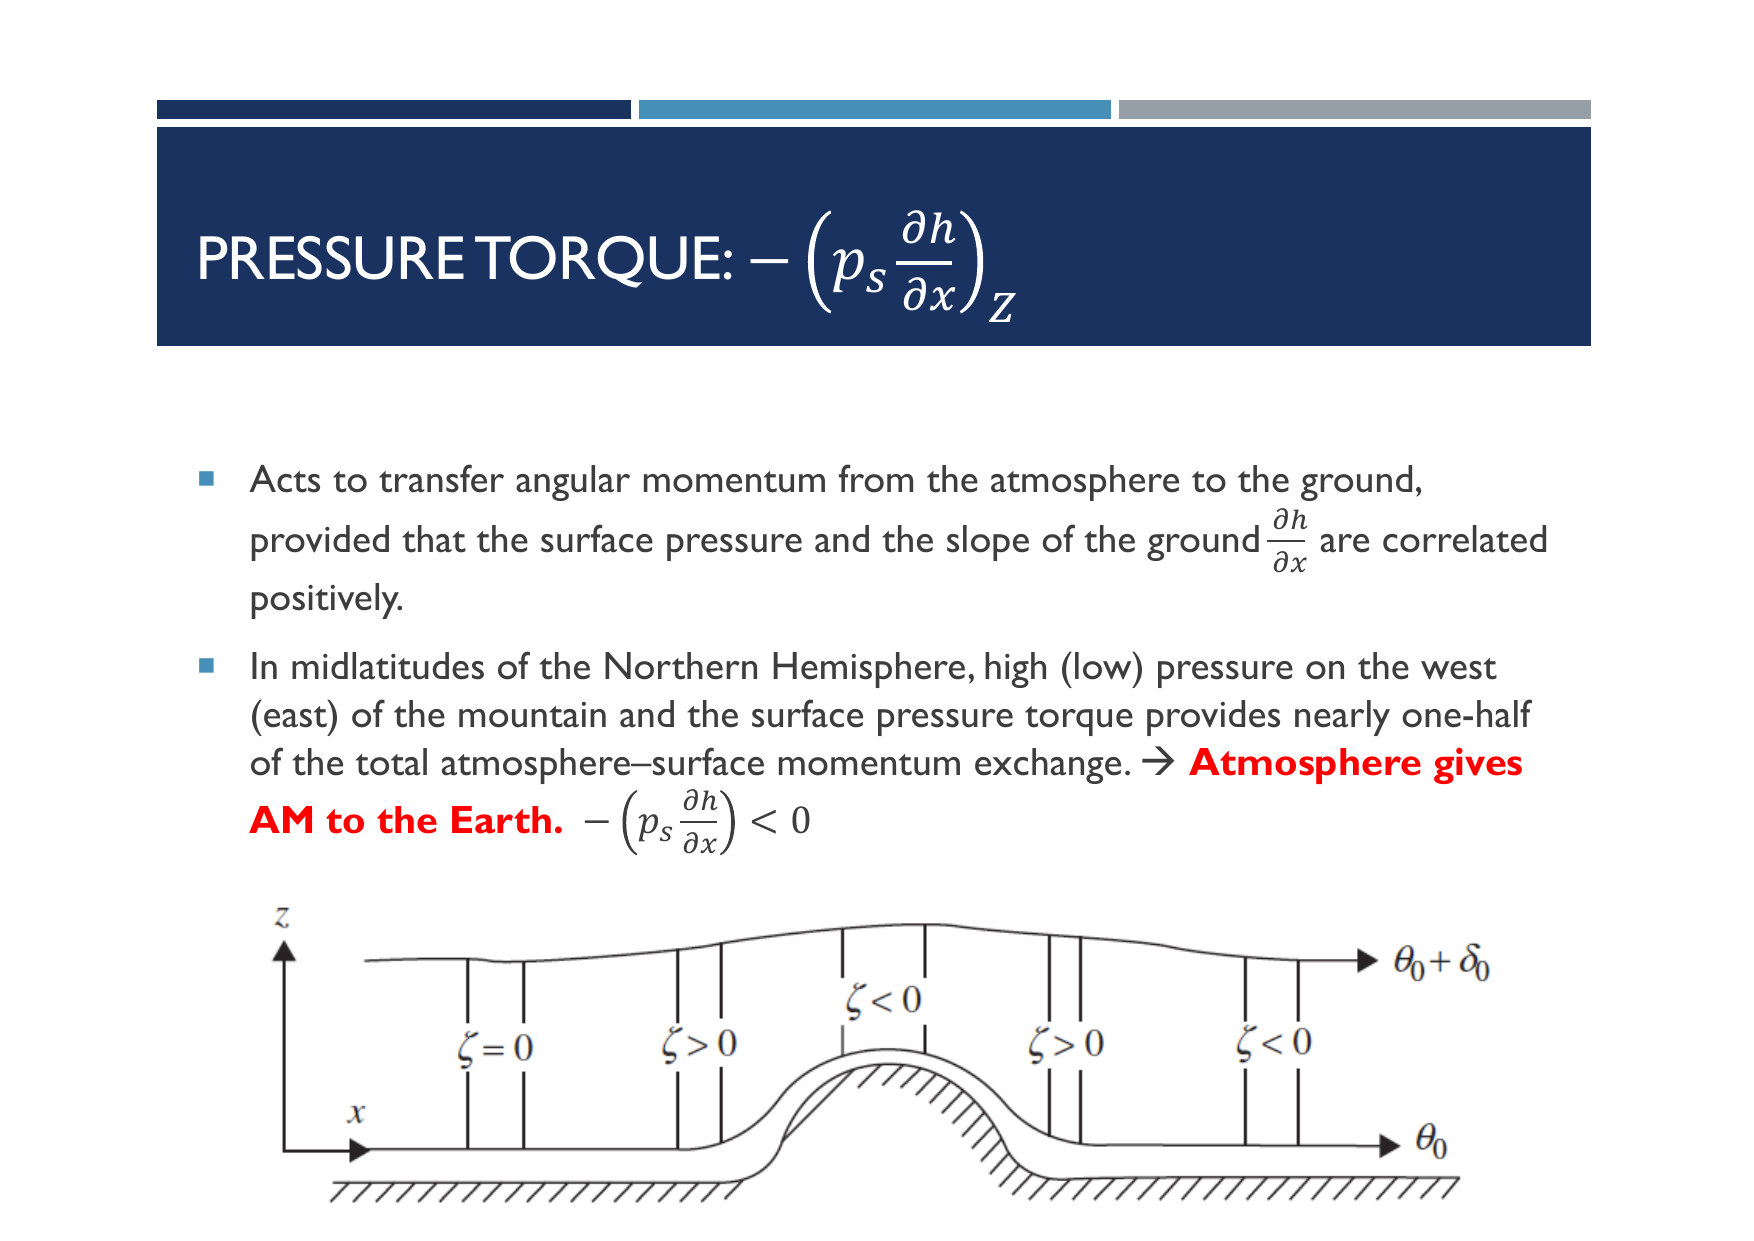
\includegraphics[width=0.85\textwidth]{images/ch07/p27_img01.png}
  \caption{Schematic of pressure (mountain) torque in the NH midlatitudes.
  Westerly mean flow encounters a meridional mountain ridge; high surface
  pressure piles up on the windward (west) side and low pressure develops
  on the lee (east) side.  The resulting east-west pressure asymmetry exerts
  an eastward force on the mountain and an equal-and-opposite westward
  force on the atmosphere, transferring westerly angular momentum from
  atmosphere to solid Earth.
  \hisu{서쪽 high, 동쪽 low가 산을 동쪽으로 미는 form drag.
  반작용으로 대기는 서방향 AM을 지구에 넘긴다.
  NH 중위도 AM 교환의 약 50\%를 이 mechanism이 담당.}}
  \label{fig:ch07_torque_mountain_schematic}
\end{figure}

산악 torque는 \textit{NH 중위도에서 특히 크다} — Rocky, Himalaya, Andes 등의
남북 방향 산맥과 그 위를 통과하는 정상 행성파 (Ch.~6 §1의 stationary wave)가
영구적인 동서 압력 비대칭을 유지하기 때문이다.  관측에 의하면 NH 중위도
westerly 영역에서 대기 → 지구 AM 전달의 약 \textbf{50\%}가 이 mountain
torque로 설명된다 (Peixoto \& Oort 1992, Ch.~11.4).  나머지 절반은
다음에 보는 마찰 torque가 담당한다.

\begin{hisublock}
Peixoto \& Oort (1992) Table~11.3, Fig.~11.16에 보고된 zonal-mean mountain
torque는 NH 30--60$^\circ$ 영역에서 음수 ($\sim -5\times 10^{18}$ N\,m)로
westerly AM이 대기로부터 지구로 흘러나간다는 직접 증거다.
본 책 \eqref{eq:ch07_torque_mountain_def}의 부호 규약과 일관된다.
SH는 산이 적어 mountain torque가 NH의 1/3 수준에 그치며, 따라서 SH AM
교환은 거의 전적으로 마찰 torque로 결정된다.
\end{hisublock}

% --------------------------------------------------------------------------
\subsubsection{Frictional (Surface Stress) Torque}

두 번째 torque mechanism은 \textgr{surface stress} ($\tau_E^x$)이다.
이것은 boundary layer turbulence가 지표면에 가하는 동방향 응력이며,
스칼라 부호는 \textit{지표 부근 zonal wind와 반대}이다.  대기 입장에서
$\tau_E^x$는 운동량을 \textit{잃는} 항이므로 zonal momentum equation의
$F_\lambda \sim -\partial \tau_E^x/\partial p$ 형태로 들어간다 (Ch.~4 §2.2 참고).

\begin{definition}[Frictional (Surface Stress) Torque]\label{def:ch07_torque_friction}
지표 ($\sigma = 1$)에서의 zonal-mean eastward stress를 $(\tau_E^x)_Z|_{\sigma=1}$
이라 하면, vertically integrated AAM budget에 기여하는 마찰 torque는
\begin{equation}\label{eq:ch07_torque_friction_def}
  T_F(\phi)
   \;=\;
   -\,a\cos\phi\,(\tau_E^x)_Z\Bigl|_{\sigma=1}.
\end{equation}
부호 규약은 mountain torque와 같다: $T_F < 0$이면 대기 → 지구.
\end{definition}

Bulk aerodynamic formula로 표면응력을 근사하면
\begin{equation}\label{eq:ch07_torque_bulk}
  \tau_E^x \;\approx\; \rho_a C_D |V_{10}|\,u_{10},
  \qquad C_D \sim 10^{-3},
\end{equation}
여기서 $u_{10}$는 10\,m altitude의 zonal wind 성분이다.  따라서 $\tau_E^x$는
$u_{10}$과 같은 부호를 가진다.  $T_F$의 부호는 $-(\tau_E^x)_Z$와 같으므로
지표 wind의 부호에 따라 결정된다:

\begin{itemize}
  \item \textbf{Trade-wind belt} ($\lvert\phi\rvert \lesssim 30^\circ$):
    surface easterly ($u_{10} < 0$) $\Rightarrow$ $\tau_E^x < 0$ $\Rightarrow$
    $T_F > 0$ — 대기가 지구로부터 AM을 \textbf{얻는다} (sink of westerly AM
    from atmosphere viewpoint reversed).  실제로는 동풍을 더 강한 동풍으로
    유지하는 것이 아니라 지구의 자전이 대기에 westerly AM을 ``주입''하는
    구조이다.
  \item \textbf{Westerly belt} ($\lvert\phi\rvert \gtrsim 30^\circ$):
    surface westerly ($u_{10} > 0$) $\Rightarrow$ $\tau_E^x > 0$ $\Rightarrow$
    $T_F < 0$ — 대기는 westerly AM을 지구에 \textbf{잃는다}.
\end{itemize}

\begin{theorem}[Hemispheric Imbalance of Frictional Torque]\label{thm:ch07_torque_friction_balance}
관측된 surface wind 분포는 무역풍대의 적분 동풍 강도와 중위도 westerly
적분 강도가 비슷한 크기를 갖도록 자연스럽게 조정된다.  그 결과,
hemispheric integral of \eqref{eq:ch07_torque_friction_def}는
\textit{0에 가까운 잔차}로 마무리되며, 잔차는 angular momentum의 장기적
저장량 변화 (또는 mountain torque와의 상쇄)에 흡수된다.
\end{theorem}

\hisu{무역풍대에서 + 중위도에서 - 의 마찰 torque 분포가 자연 조정되어
hemispheric residual은 거의 0.  이것이 LOD-AAM의 장기적 안정성의 근원.}

\begin{remark}[Why Friction Dominates in the SH and Tropics]
SH는 해양이 우세하고 큰 산맥이 적기 때문에 mountain torque가 작다.
따라서 SH에서는 거의 \textit{전적으로 marichal torque}만이 대기-지구 AM
교환을 매개한다.  열대는 산이 거의 없고 surface easterly가 매우 강하므로
역시 마찰 torque가 지배적이다.  Mountain torque의 영향력은 NH midlatitude에
거의 국한된다.
\end{remark}

\begin{hisublock}
세 종류 torque의 상대적 기여를 한 줄로 요약:
\begin{itemize}
  \item \textbf{Tropics}: 마찰 torque (+) 지배. Mountain torque 무시 가능.
  \item \textbf{NH midlatitudes}: 마찰 torque ($-$) $\approx$ Mountain torque ($-$)
    $\sim 50\%$ each. 이 둘이 함께 mid-latitude westerly AM sink 역할.
  \item \textbf{SH midlatitudes}: 마찰 torque ($-$) 지배. Mountain torque는
    NH의 1/3 정도.
  \item \textbf{High latitudes ($>$60$^\circ$)}: weak surface easterly →
    weak (+) 마찰 torque. Mountain torque도 약함.
\end{itemize}
Holton \& Hakim (5th ed.) Ch.~10.4에서도 같은 hemispheric asymmetry를
강조한다.
\end{hisublock}

% --------------------------------------------------------------------------
\subsubsection{Mountain Torque Geometry: A Merry-Go-Round Picture}

산악 torque를 더 직관적으로 이해하기 위해 다음과 같은 \textit{merry-go-round}
유추를 사용한다.  남북으로 늘어선 두 개의 idealized 산 (Mountain I, II)이
있다고 가정하고, 각 산의 \textit{서쪽}과 \textit{동쪽} 측면에서의 압력을
$p_W^1, p_E^1, p_W^2, p_E^2$로 각각 표시한다.

\begin{figure}[ht]
  \centering
  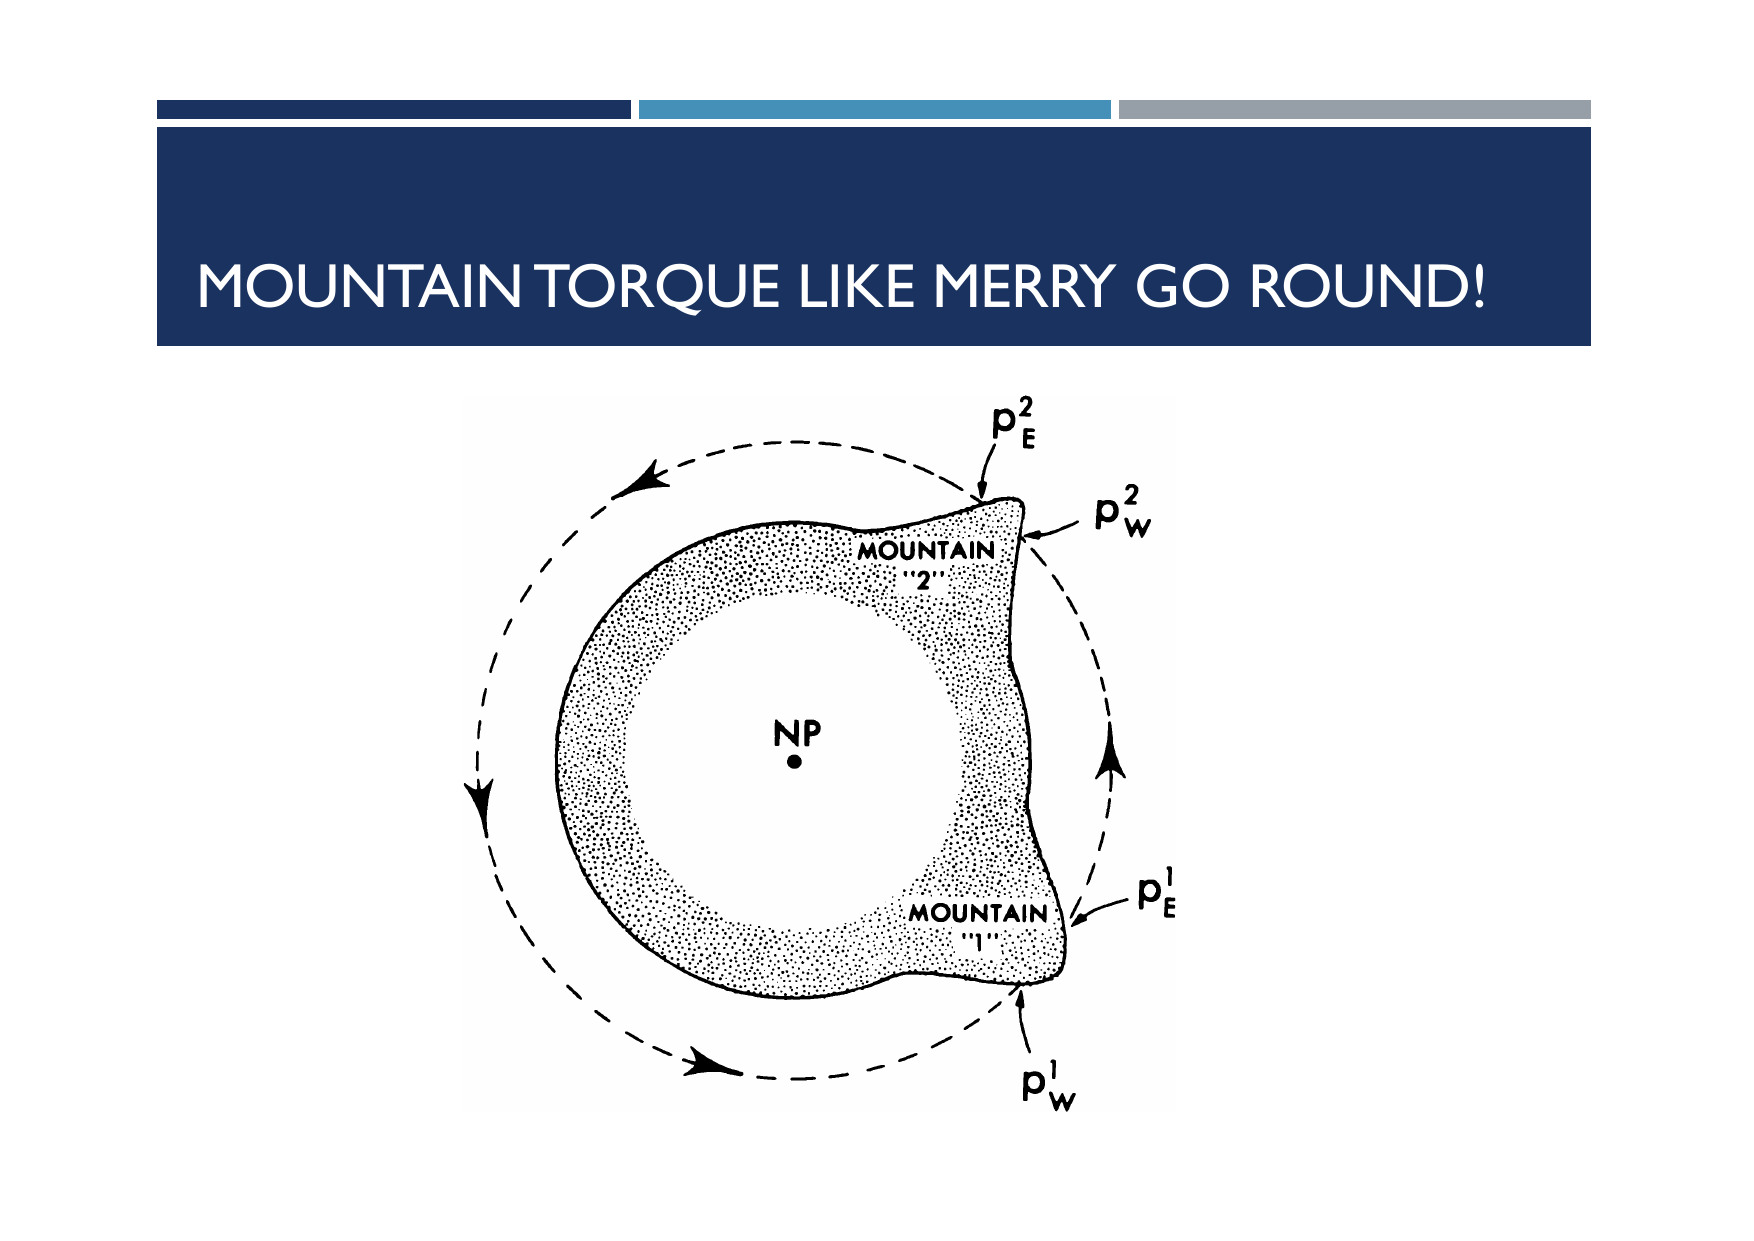
\includegraphics[width=0.85\textwidth]{images/ch07/p29_img01.png}
  \caption{Merry-go-round picture of mountain torque.  Two idealized
  mountains (Mountain~I and Mountain~II) with pressures
  $p_W^1, p_E^1$ on the west and east faces of Mountain~I, and
  $p_W^2, p_E^2$ on Mountain~II.  The net torque on the solid earth from
  the atmosphere is proportional to $(p_W - p_E)$ summed over all mountains;
  when this sum is positive (high to the west, low to the east), the
  atmosphere imparts an eastward force on the mountain and loses westerly
  angular momentum.
  \hisu{산 양쪽 압력차의 합이 산악 torque의 부호를 결정.
  서쪽 high - 동쪽 low면 대기가 산을 동쪽으로 밀어 서풍 AM을 잃는다.}}
  \label{fig:ch07_torque_merrygoround}
\end{figure}

각 산이 받는 net eastward force는 $(p_W^i - p_E^i)\,A_i$ ($A_i$는 산의
유효 단면적)이며, 모든 산을 합하면 latitude circle 전체에 대한
$-(p_s\,\partial h/\partial x)_Z$의 zonal integral이 된다.  이로써
\eqref{eq:ch07_torque_mountain_def}와 같은 결과가 회복된다.

\begin{remark}[Stationary Wave–Mountain Coupling]\label{rem:ch07_torque_stationary}
Ch.~6 §1에서 본 stationary wave는 산 위에서 \textit{진폭이 크고 위상이
고정}되어 있다.  이 정상파의 trough/ridge가 산 양쪽 압력 비대칭을 영구적으로
유지하므로 mountain torque의 시간 평균이 0이 되지 않는다.  즉, 산악 torque는
\textbf{stationary eddy의 직접적 manifestation}이다.
\end{remark}

\hisu{산악 torque $\equiv$ stationary wave의 결과.
travel하는 transient wave는 시간평균하면 산악 torque 기여가 작다.}

% --------------------------------------------------------------------------
\subsubsection{Gravity Wave Drag over Orography}

산이 \textit{대기와 AM을 교환}하는 또 다른 경로는 \textgr{internal gravity waves}이다.
안정한 성층 상태의 대기가 산을 넘을 때, 산을 lower boundary 강제력으로 받는
\textit{vertically propagating gravity wave}가 발생한다.  이 wave는 운동량을
연직 상방으로 수송하며, 결국 stratosphere 또는 mesosphere에서 critical layer
absorption이나 wave breaking을 통해 \textit{흩어진다}.  그 결과 산은 대기에서
westerly AM을 \textbf{흡수}하고, 이 흡수가 일어나는 고도까지 \textit{운동량을
원격으로 추출}한다.

\begin{figure}[ht]
  \centering
  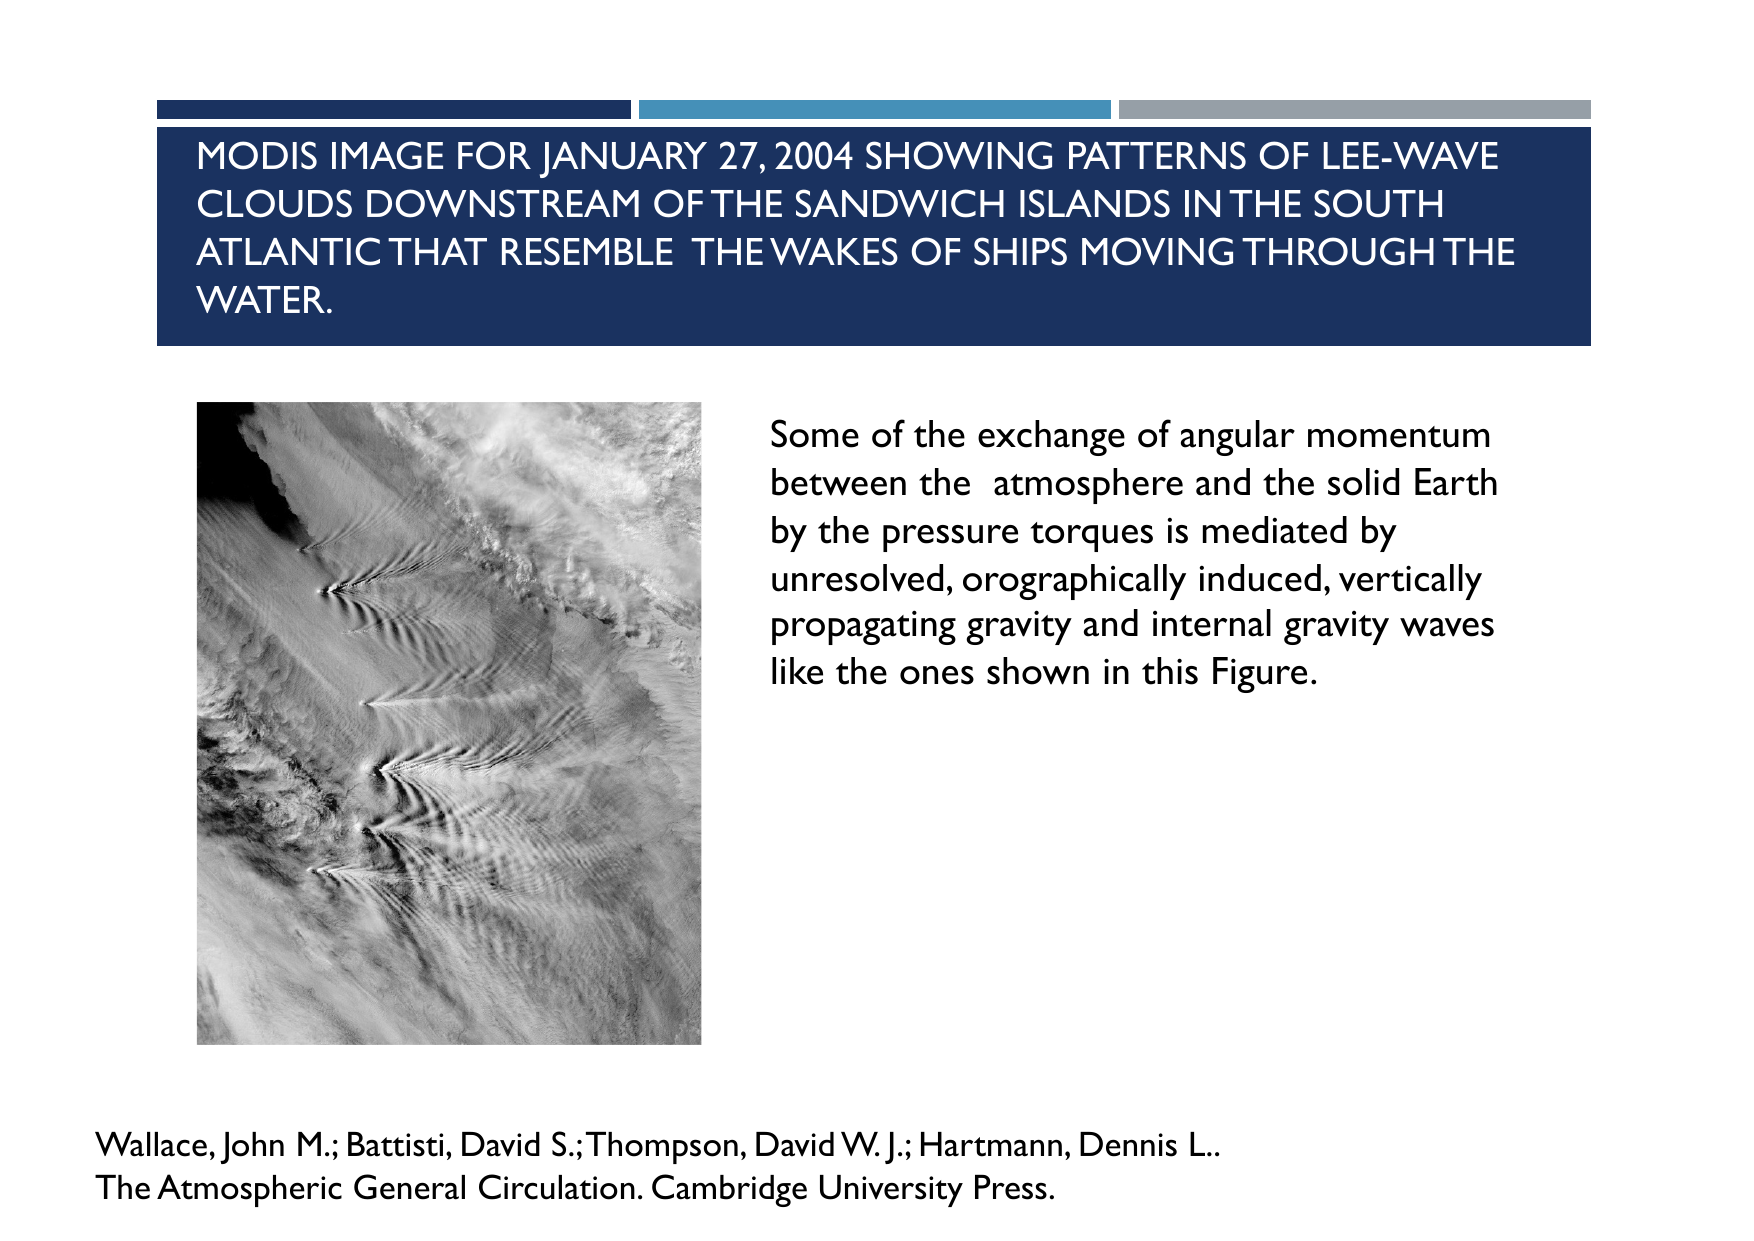
\includegraphics[width=0.85\textwidth]{images/ch07/p30_img01.png}
  \caption{MODIS satellite image (27 January 2004) showing lee-wave clouds
  downstream of the South Sandwich Islands.  Each parallel cloud band marks
  the crest of a vertically propagating internal gravity wave excited by
  westerly flow over the islands.  Even from these small isolated features,
  significant vertical momentum flux escapes upward into the stratosphere,
  where it is deposited as a westward (decelerating) force on the mean flow.
  \hisu{MODIS Sandwich Islands lee-wave cloud (2004년 1월 27일).
  작은 섬도 strato까지 운동량을 전달한다 — 산만 산이 아니다.}}
  \label{fig:ch07_torque_modis_sandwich}
\end{figure}

\begin{figure}[ht]
  \centering
  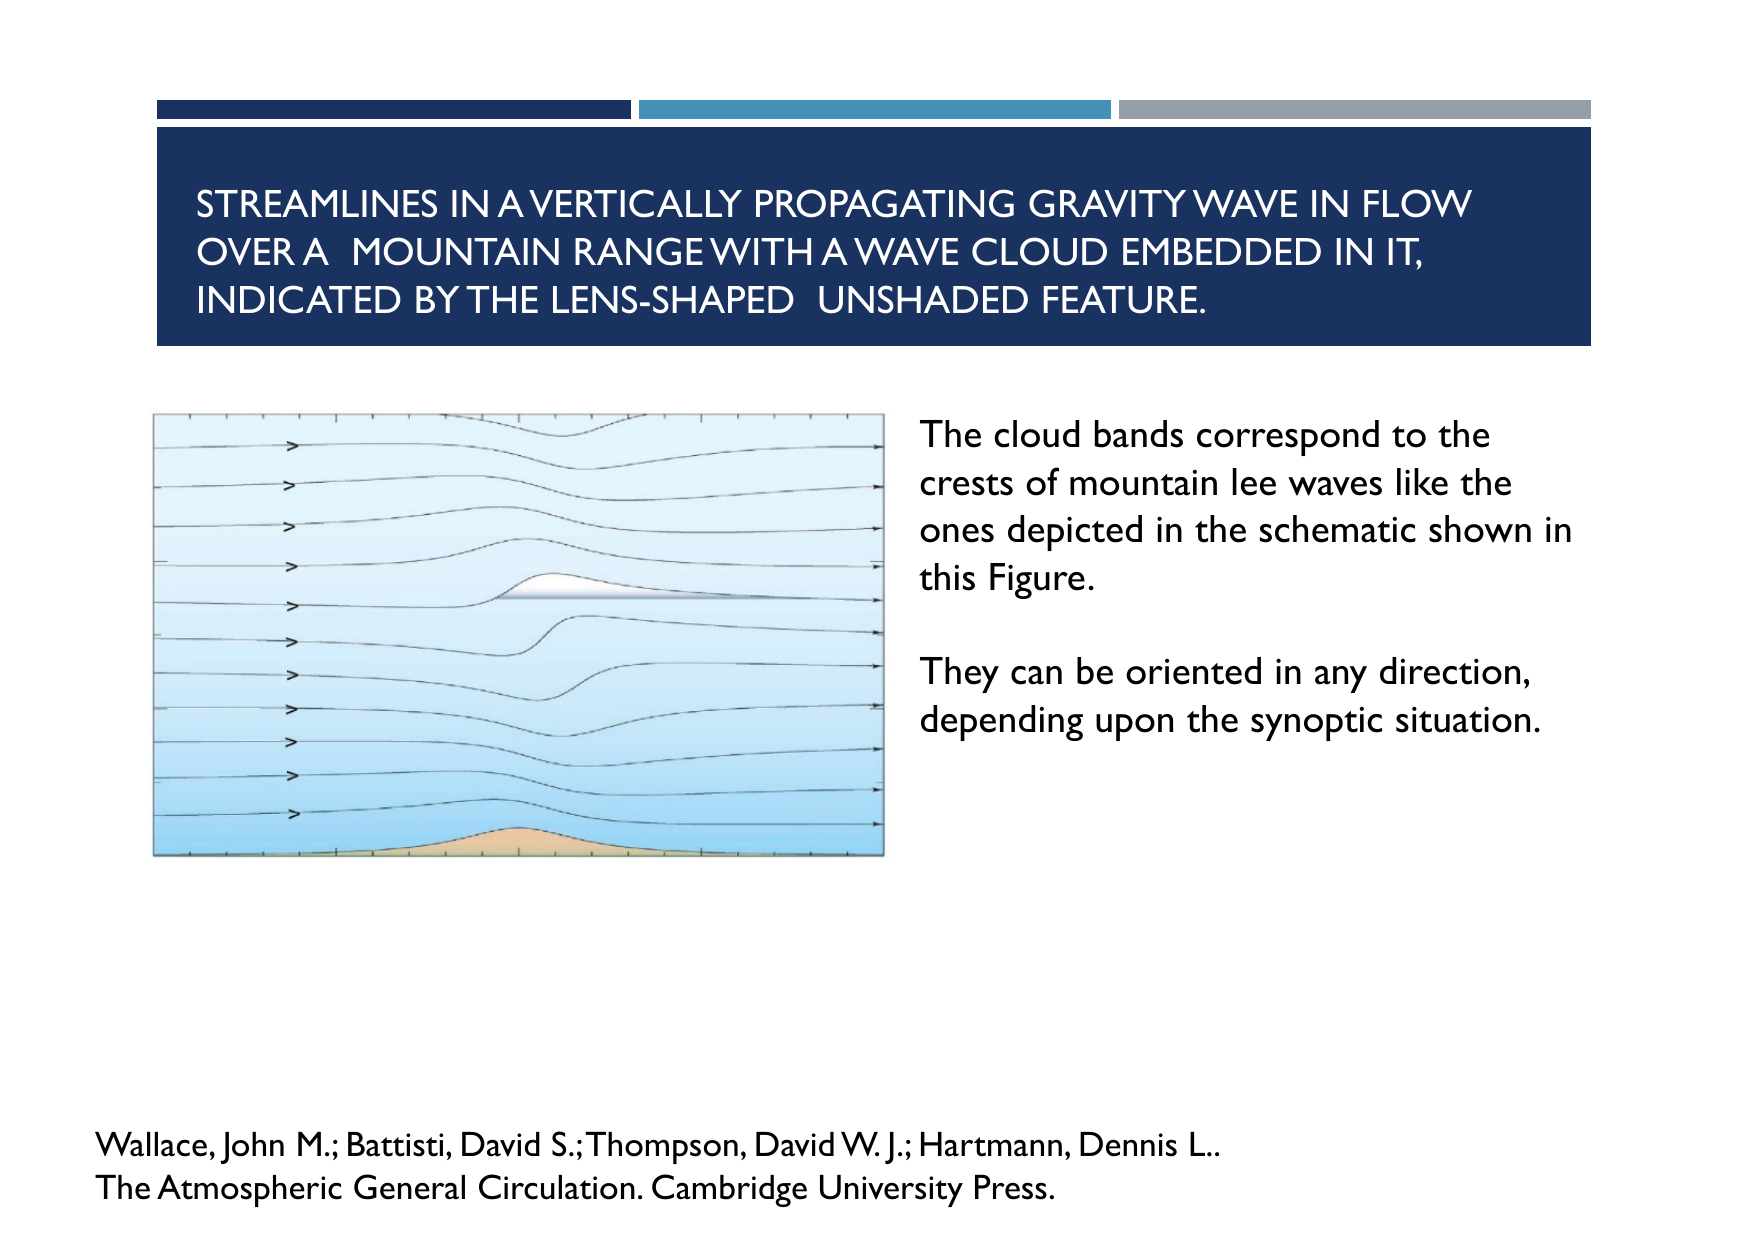
\includegraphics[width=0.85\textwidth]{images/ch07/p31_img01.png}
  \caption{Schematic of streamlines (solid) and isentropes (dashed) in a
  stably stratified flow over an isolated mountain.  Air is forced upward on
  the windward slope and oscillates with the Brunt--V\"ais\"al\"a frequency
  on the lee side, generating a train of stationary lee waves and a vertical
  flux of westward (negative $u$) momentum.  The lens-shaped cap cloud and
  rotor cloud are common visual signatures.
  \hisu{성층 안정 + 산 = 정지파 (lee wave).
  산은 운동량을 위로 ``쏘아 올린다''.}}
  \label{fig:ch07_torque_lee_schematic}
\end{figure}

\begin{definition}[Gravity Wave Drag]\label{def:ch07_torque_gwd}
산악으로부터 위로 전파되는 internal gravity wave는 운동량 flux
\begin{equation}\label{eq:ch07_torque_gwd_flux}
  \tau_{GW}(z)
  \;=\;
  \rho\,(u_E\,w_E)_Z
\end{equation}
를 운반한다.  Non-dissipative한 영역에서는 $\tau_{GW}$가 높이에 따라
\textit{보존}되며, wave breaking 또는 critical layer absorption이 일어나는
고도 $z_*$에서 갑작스러운 발산이 발생하여
\begin{equation}\label{eq:ch07_torque_gwd_decel}
  F_{GW} \;=\; -\frac{1}{\rho}\frac{\partial \tau_{GW}}{\partial z}\Bigl|_{z=z_*}
\end{equation}
의 zonal force를 zonal mean flow에 가한다.
\end{definition}

\hisu{Gravity wave drag: 산이 만든 wave가 한참 위 (성층권/중간권)에서 깨지면서
운동량을 빼앗는다.  ``원격 mountain torque''라 불러도 좋다.}

\begin{remark}[Why GW Drag Matters for Climate Models]\label{rem:ch07_torque_gwd_models}
GCM의 격자 해상도 ($\sim$50--100\,km)로는 sub-grid scale 산악 ($\sim$1--50\,km)이
직접 분해되지 않는다.  따라서 모델은 \textit{명시적으로} \eqref{eq:ch07_torque_gwd_decel}를
parameterize해야 하며, 이를 빼면 stratosphere의 polar night jet이 과도하게
강하게 모의되는 \textit{cold-pole bias}가 발생한다.  Andrews, Holton, Leovy
(1987) Ch.~7.4가 표준 reference이다.
\end{remark}

\begin{hisublock}
\textbf{핵심 메시지}: 구름이 보이지 않는 맑은 날에도 산 위에서는 gravity wave가
끊임없이 발생하고 있다.  육안으로 cap cloud나 rotor cloud가 안 보여도 (성층이
적당히 stably stratified이면), 산은 대기로부터 westerly AM을 \textbf{빼앗고
있다}.  결국 mountain torque는 (i) 직접 압력차에 의한 form drag (지표 근처에서
작용) + (ii) gravity wave를 통한 상부 대기 운동량 흡수 — 두 path가 합쳐진
복합 mechanism이다.  GCM에서 (ii)를 빼면 stratospheric jet이 잘못 모의된다는
사실은 이 ``보이지 않는'' torque의 정량적 중요성을 보여준다.
\end{hisublock}

% =============================================================================
%   SECTION 4 — Poleward Transport of Atmospheric Angular Momentum
% =============================================================================

\subsection{Poleward Transport of Atmospheric Angular Momentum}

\S3에서 우리는 대기와 지구가 어떻게 AM을 교환하는지 보았다.  결론적으로
열대 (무역풍대)는 atmosphere가 AM을 \textbf{얻는} source 지역이고, 중위도
westerly 영역은 atmosphere가 AM을 \textbf{잃는} sink 지역이었다.
그러나 zonal-mean climatology가 시간에 대해 거의 정상상태인 사실로부터
\textit{각 위도 ring 안의 AM이 시간에 따라 일정}하다는 것을 알 수 있고,
따라서 source 영역의 AM은 어떻게든 sink 영역으로 \textbf{지속적으로 수송}되어야
한다.

\begin{theorem}[Necessity of Poleward AAM Transport]\label{thm:ch07_trans_necessity}
관측된 surface wind 분포 (열대 east, 중위도 west)와 stationarity 조건 하에서,
대기는 \textbf{각 열대 (sub-Hadley)에서 중위도로 향하는 net poleward angular
momentum flux}를 가져야 한다.  이 flux의 크기는 두 source/sink 영역의
torque integral과 정확히 균형을 이룬다.
\end{theorem}

\hisu{핵심 명제: 적도는 AAM source, 중위도는 sink, 따라서 적도 → 극으로
끊임없는 운동량 수송이 필요하다.}

% --------------------------------------------------------------------------
\subsubsection{Surface Wind Patterns: The Source/Sink Structure}

\begin{figure}[ht]
  \centering
  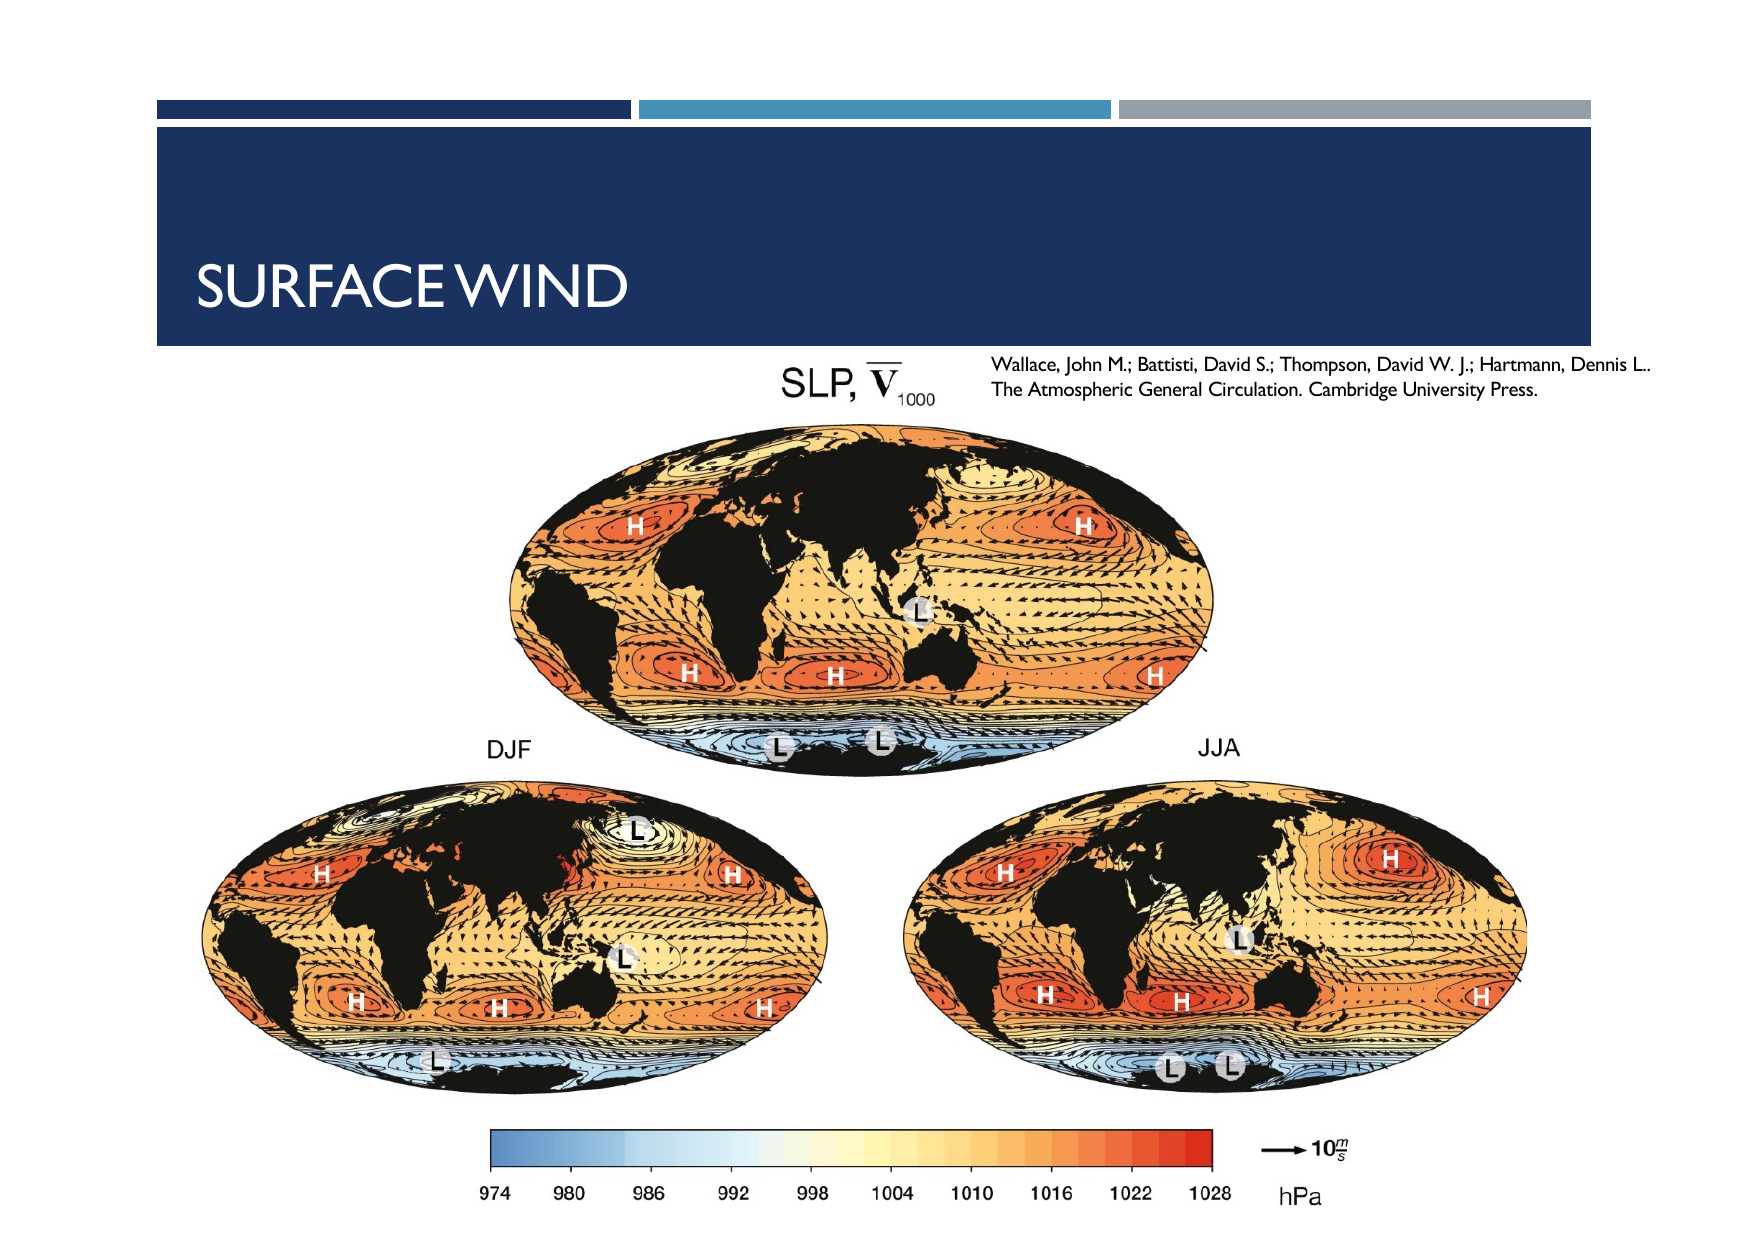
\includegraphics[width=0.85\textwidth]{images/ch07/p33_img01.png}
  \caption{Climatological sea level pressure (contours) and near-surface
  (1000\,hPa) wind vectors for DJF (top) and JJA (bottom).  Three
  zonally-averaged regimes stand out: the equatorial easterly trade-wind
  belt converging at the ITCZ, the subtropical highs near $\pm 30^\circ$,
  and the midlatitude westerlies poleward of $\sim 30^\circ$.  These three
  bands provide the source ($\lvert\phi\rvert<30^\circ$) / sink
  ($\lvert\phi\rvert>30^\circ$) structure for atmospheric angular momentum.
  \hisu{SLP + 지표풍 분포.  무역풍대 (적도 양쪽 0--30$^\circ$) =
  AAM source, 중위도 서풍대 (30--60$^\circ$) = AAM sink, ITCZ + 아열대고기압이
  경계.}}
  \label{fig:ch07_trans_surface_wind}
\end{figure}

Figure~\ref{fig:ch07_trans_surface_wind}에서 보는 \textit{universal}
surface wind structure는 다음과 같이 요약된다:

\begin{itemize}
  \item \textbf{Trade winds} ($0$--$30^\circ$): persistent easterlies.
    $\tau_E^x < 0$ ($u_{10} < 0$) 이므로 \eqref{eq:ch07_torque_friction_def}
    에서 $T_F > 0$ — 대기가 지구로부터 westerly AM을 얻는다.
  \item \textbf{Westerly belt} ($30$--$60^\circ$): persistent westerlies.
    $\tau_E^x > 0$ 이므로 $T_F < 0$ — 대기는 westerly AM을 지구에 잃는다.
  \item \textbf{ITCZ} (적도): 두 무역풍의 수렴대.  $u_{10} \approx 0$
    이므로 마찰 torque는 0에 가깝지만 vertical convection이 활발하여
    AM의 vertical redistribution이 일어난다.
  \item \textbf{Subtropical highs} ($\sim 30^\circ$): 이 위도가 정확히
    source/sink 경계, 즉 $T_F = 0$ 인 위도이다.
\end{itemize}

\begin{remark}[Universality on Aquaplanet]\label{rem:ch07_trans_aquaplanet}
대륙과 산이 모두 없는 \textgr{aquaplanet} 시뮬레이션에서도 정확히 같은
3-band surface wind 구조가 나타난다 (Williamson et al.\ 2012; Marshall \&
Plumb 2008).  이는 source/sink structure가 \textit{회전 + 차등 가열}만으로도
자동적으로 생긴다는 universal property임을 보여준다.
\end{remark}

% --------------------------------------------------------------------------
\subsubsection{The Tropical–Extratropical Balance}

source와 sink가 latitude로 분리되어 있으므로, 두 영역을 잇는
\textit{meridional transport}가 필요하다.  이 수송은 두 가지 mechanism의
조합이다:

\begin{itemize}
  \item \textbf{Hadley/Ferrel/Polar mean meridional circulation (MMC)}: 열대
    Hadley cell이 surface에서 적도 방향 (low-AM 공기)을 가져오고 상층에서
    극 방향 (high-AM 공기)을 가져간다.
  \item \textbf{Eddy momentum flux}: midlatitude transient eddy ($u_E v_E$)
    가 net 극 방향 운동량 수송을 담당.  특히 30--60$^\circ$의 sink
    영역에서 지배적.
\end{itemize}

\begin{figure}[ht]
  \centering
  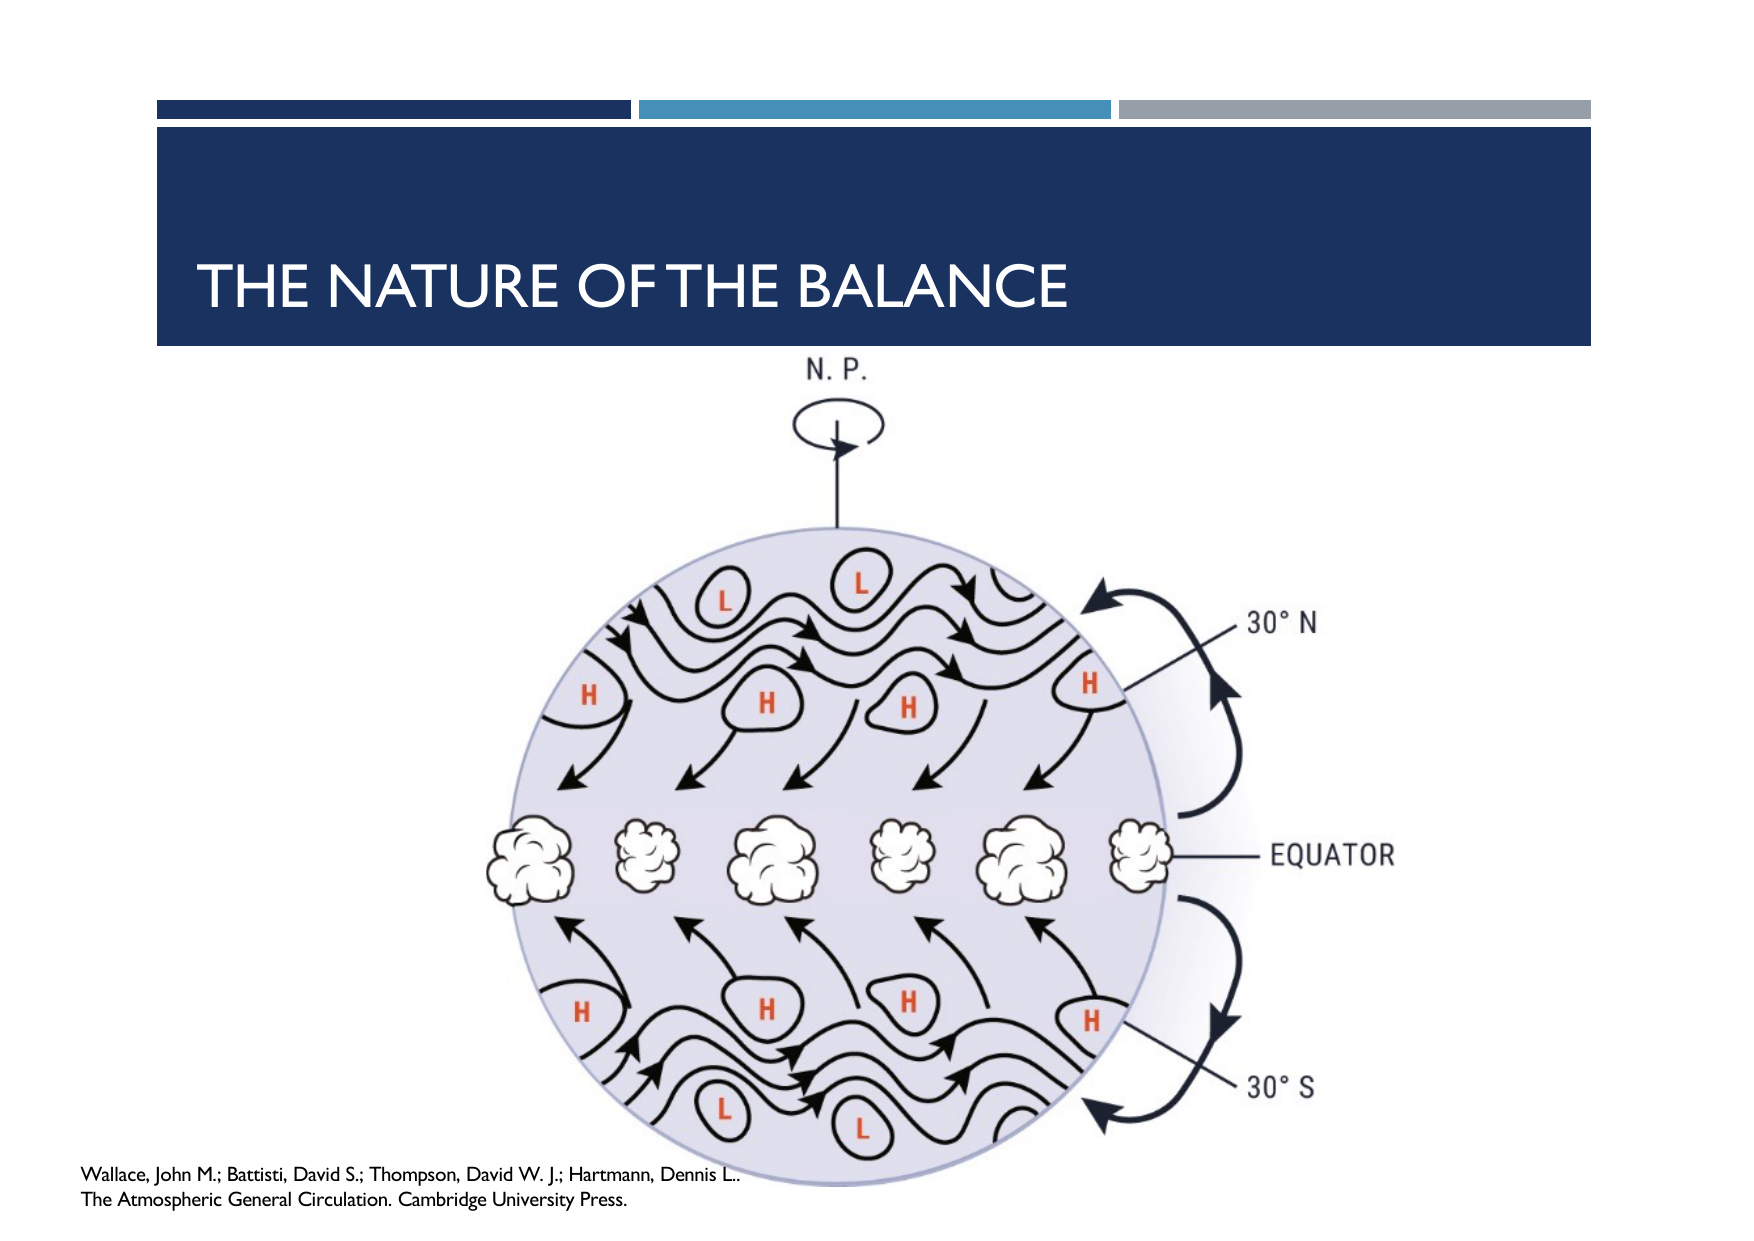
\includegraphics[width=0.85\textwidth]{images/ch07/p35_img01.png}
  \caption{Schematic of the three-cell meridional circulation in each
  hemisphere — Hadley (low latitudes), Ferrel (midlatitudes), and Polar
  cells — together with the surface pressure pattern (subpolar L, subtropical
  H) and dominant eddy fluxes.  Mass rises at the equator and near
  $60^\circ$, sinks near $30^\circ$ and the poles.  Hadley cell carries
  high-AM upper-tropospheric air poleward; eddies carry AM further poleward
  in midlatitudes against the Ferrel cell's near-surface mass flow.
  \hisu{Hadley / Ferrel / Polar 3-cell + 지표 H/L + 에디 흐름.
  Hadley는 직접순환, Ferrel은 간접순환 — Ferrel cell은 에디가 강제한다.}}
  \label{fig:ch07_trans_three_cell}
\end{figure}

\begin{figure}[ht]
  \centering
  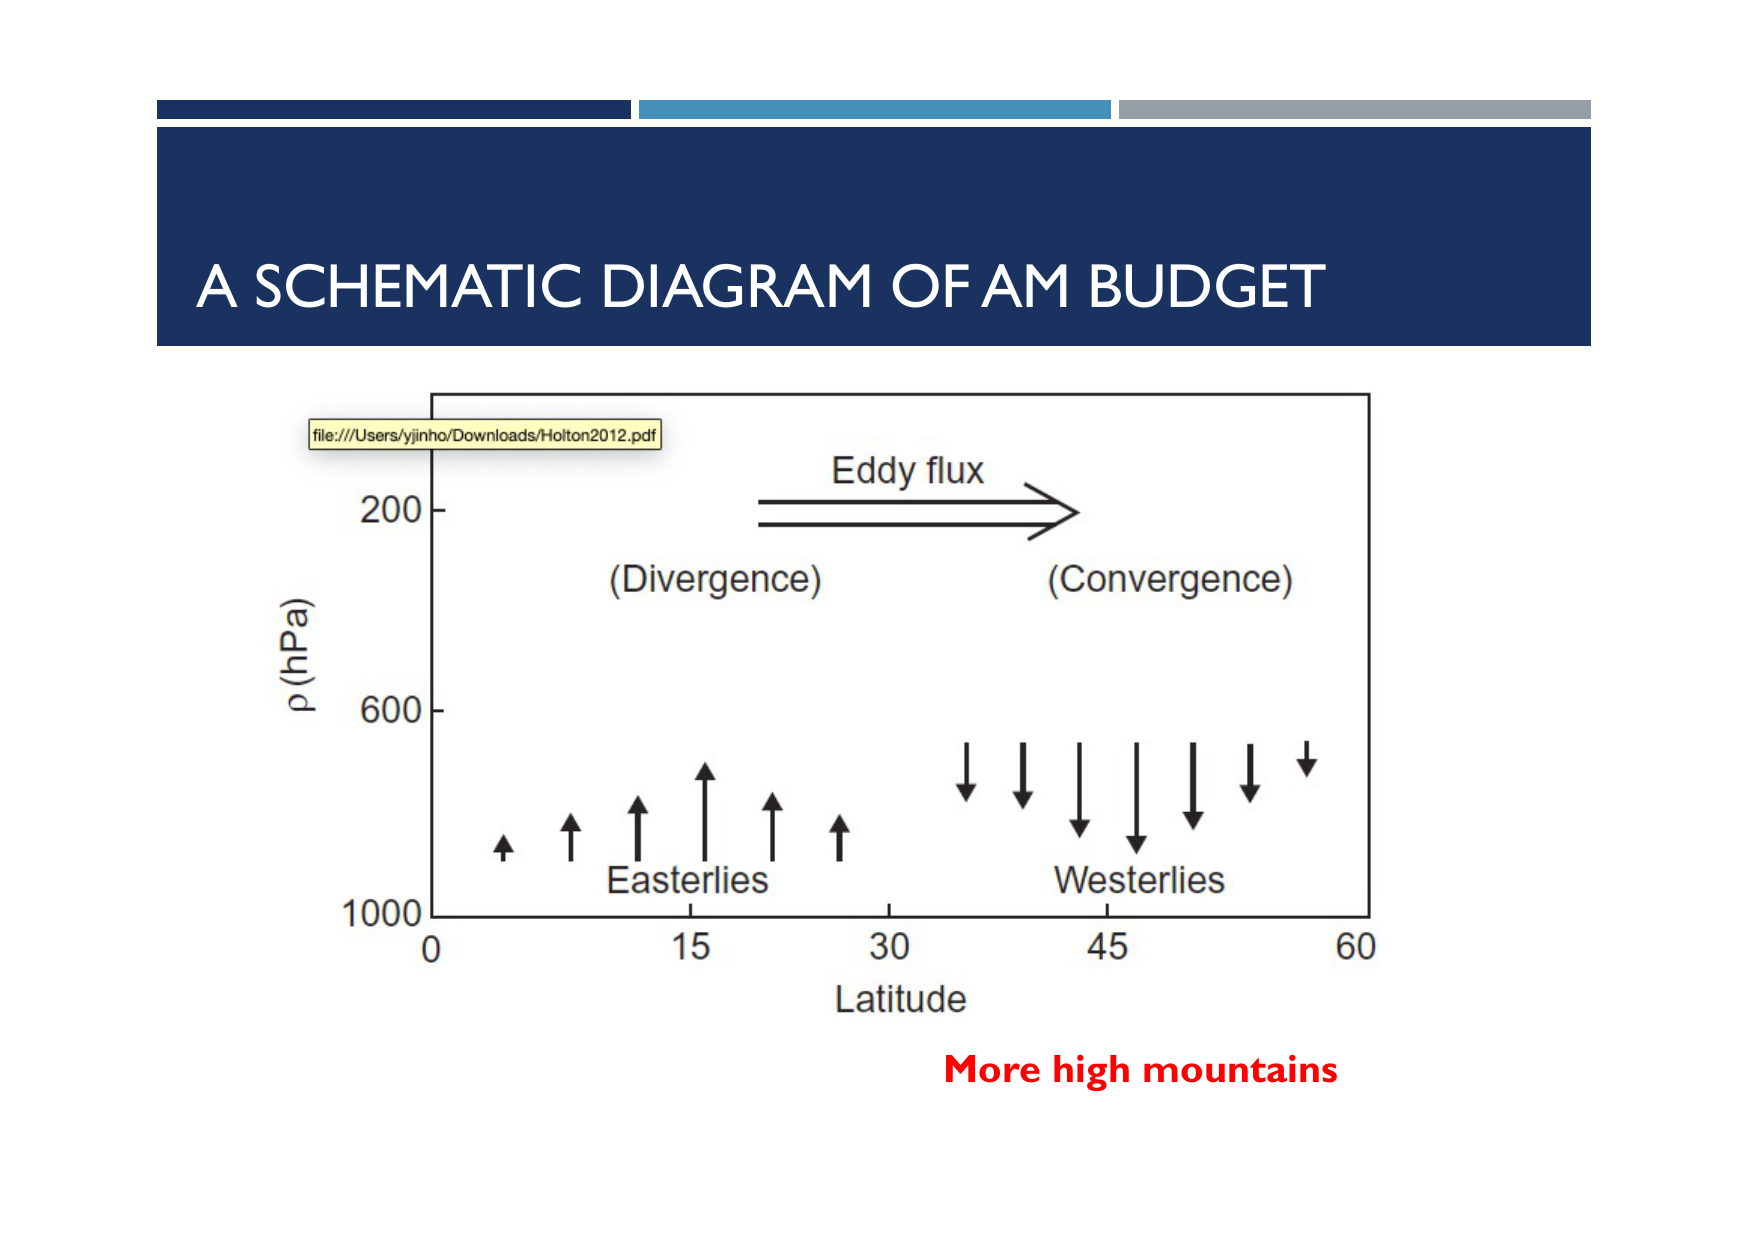
\includegraphics[width=0.85\textwidth]{images/ch07/p36_img01.png}
  \caption{Zonally averaged angular momentum budget schematic.  In the
  tropics ($0$--$30^\circ$) surface easterlies pump westerly AM into the
  atmosphere (divergence of meridional flux); in the midlatitudes
  ($30$--$60^\circ$) surface westerlies remove AM from the atmosphere
  (convergence).  Eddy flux arrows close the budget by transporting AM from
  source to sink.
  \hisu{단순화한 AM 수지: 0--30$^\circ$는 source (지표 동풍),
  30--60$^\circ$는 sink (지표 서풍), 에디가 둘을 연결.}}
  \label{fig:ch07_trans_budget_schematic}
\end{figure}

\hisu{Aquaplanet에서도 같은 결과가 나오므로 이것은 \textbf{지구 회전체의
universal property}.}

% --------------------------------------------------------------------------
\subsubsection{The Long-Term Two-Term Balance}

\eqref{eq:ch07_cons_threeterm}의 세 항 — meridional flux convergence,
mountain torque, friction torque — 가운데, \textit{장기 평균} (annual 또는
multi-year mean)에서는 mountain torque가 다른 두 항보다 \textbf{작은} 잔차
항으로 작용한다는 것이 관측 결과이다.  따라서 다음 근사가 성립한다:

\begin{equation}\label{eq:ch07_trans_two_term}
  \boxed{
  -\frac{1}{g\cos\phi}\frac{\partial}{\partial y}
   \int_0^1 (p_s M v)_Z\cos\phi\,d\sigma
  \;\;\approx\;\;
   a\cos\phi\,(\tau_E^x)_Z\Bigl|_{\sigma=1}.
  }
\end{equation}

\begin{theorem}[Two-Term Long-Term AAM Balance]\label{thm:ch07_trans_two_term}
다년 평균 zonal AAM budget은 \textbf{meridional flux convergence}와
\textbf{surface stress torque}의 두 항으로 거의 완벽히 닫힌다.
\end{theorem}

\hisu{Mountain torque는 NH midlatitude에서 큰 instantaneous 신호를 주지만
장기 평균에서는 두 다른 항보다 작은 잔차에 그친다.  Source/sink balance의
``양대 산맥''은 (i) 마찰 torque와 (ii) 자오 AM flux convergence이다.}

% --------------------------------------------------------------------------
\subsubsection{Decomposition into Solid-Rotation, Drift, and Eddy Fluxes}

이제 meridional AAM flux $\int_0^1 (p_s M v)_Z\,d\sigma$의 \textit{구조}를
파헤친다.  먼저 zonal-mean / eddy 분해를 변수별로 정의한다:
\begin{align}
  M &= M_Z + M_E
     = \bigl(\Omega a\cos\phi + u_Z + u_E\bigr) a\cos\phi,
     \label{eq:ch07_trans_decomp_M} \\
  p_s v &= (p_s v)_Z + (p_s v)_E.
     \label{eq:ch07_trans_decomp_psv}
\end{align}
\eqref{eq:ch07_trans_decomp_M}--\eqref{eq:ch07_trans_decomp_psv}를 곱하고
zonal-mean 취하면 (cross 항 $(X_Z\cdot Y_E)_Z = 0$이므로 사라짐):
\begin{equation}\label{eq:ch07_trans_three_flux}
  (p_s M v)_Z
  \;=\;
  \underbrace{\Omega a\cos\phi\,(p_s v)_Z}_{\text{solid-rotation flux}}
  \;+\;
  \underbrace{a\cos\phi\,u_Z\,(p_s v)_Z}_{\text{mean (drift) flux}}
  \;+\;
  \underbrace{a\cos\phi\,(u_E (p_s v)_E)_Z}_{\text{eddy flux}}.
\end{equation}

\begin{remark}[Physical Meaning of Each Term]\label{rem:ch07_trans_three_meaning}
세 항은 각각 \textbf{독립적인 물리적 process}를 표현한다:
\begin{enumerate}
  \item \textbf{Solid-rotation flux} $\Omega a\cos\phi\,(p_s v)_Z$:
    회전하는 지구와 같이 움직이는 ``rigid body'' 부분의 AM 수송.
    Net 질량 수송이 latitude circle을 가로지르지 않는 조건
    (\eqref{eq:ch07_trans_continuity} 다음 항목)에서 이 항은
    \textbf{수직 적분 시 정확히 0}이 된다.
  \item \textbf{Mean (drift) flux} $a\cos\phi\,u_Z\,(p_s v)_Z$:
    zonal-mean wind $u_Z$가 zonal-mean meridional mass flux $(p_s v)_Z$에
    실려서 수송되는 AM.  Hadley cell이 활동하는 \textbf{tropics에서 중요},
    중위도 Ferrel cell의 $(p_s v)_Z$는 약하므로 작다.
  \item \textbf{Eddy flux} $a\cos\phi\,(u_E(p_s v)_E)_Z$: transient + stationary
    eddy에 의한 momentum transport.  \textbf{Midlatitudes에서 지배적}.
\end{enumerate}
\end{remark}

\hisu{3항 분해: solid (회전체) + drift (평균 흐름) + eddy.
열대는 drift 지배, 중위도는 eddy 지배.}

% --------------------------------------------------------------------------
\subsubsection{The Continuity Constraint: Why Solid-Rotation Drops Out}

\eqref{eq:ch07_trans_three_flux}의 첫 번째 항이 사라지는 이유는
\textit{질량 보존}에 있다.  Sigma 좌표 continuity equation
\begin{equation}\label{eq:ch07_trans_continuity_local}
  \frac{\partial p_s}{\partial t} + \nabla\!\cdot\!(p_s \vec{V})
  + p_s \frac{\partial \dot\sigma}{\partial \sigma} = 0
\end{equation}
을 zonal-mean 취한 후 $\sigma$에 대해 0에서 1까지 적분하면 ($\dot\sigma$가
boundary에서 0이므로 마지막 항이 사라지고):
\begin{equation}\label{eq:ch07_trans_continuity}
  \frac{\partial p_{s,Z}}{\partial t}
  \;=\;
  -\,\frac{1}{\cos\phi}\,\frac{\partial}{\partial y}
   \int_0^1 (p_s v)_Z\,\cos\phi\,d\sigma.
\end{equation}

시간평균 조건 ($\partial p_{s,Z}/\partial t = 0$ for long-term mean)을 적용하면:
\begin{equation}\label{eq:ch07_trans_mass_conservation}
   \frac{\partial}{\partial y}\!\left[
    \int_0^1 (p_s v)_Z\,\cos\phi\,d\sigma\right] = 0.
\end{equation}
이는 \textbf{모든 위도 원을 가로지르는 net mass flux가 0}임을 뜻한다 — 시간평균
관점에서 보면 각 latitude ring의 질량이 보존되어야 하기 때문이다.

\begin{theorem}[Vanishing of the Solid-Rotation Term]\label{thm:ch07_trans_solid_zero}
시간평균 조건 하에서 \eqref{eq:ch07_trans_three_flux}의 solid-rotation flux는
수직 적분 시 정확히 0이다:
\begin{equation}\label{eq:ch07_trans_solid_zero}
  \int_0^1 \Omega a\cos\phi\,(p_s v)_Z\,d\sigma
  \;=\;
  \Omega a\cos\phi \int_0^1 (p_s v)_Z\,d\sigma
  \;\stackrel{\eqref{eq:ch07_trans_mass_conservation}}{=}\; 0.
\end{equation}
\end{theorem}

\hisu{이 정리가 \S4 전체의 ``closure'': solid 회전체에 실려가는 AM 수송은
시간평균에서 사라지므로, 실제 net poleward AM 수송은 \textbf{drift + eddy}
두 항에서만 나온다.}

\begin{hisublock}
이 결과는 직관적이다.  지구 자체와 함께 도는 ``rigid body'' AM은 mass를
싣고 다니지 않는 한 latitude를 가로지를 수 없다.  시간평균 mass 보존이
그 수송 channel을 막아버리므로, $\Omega a\cos\phi$ 항은 자동적으로 사라진다.
남는 것은 (i) zonal-mean wind의 deviation부분 $u_Z$를 실어나르는 drift
(Hadley cell upper branch)와 (ii) eddy flux 두 가지 — 이 두 항을 다음
세부 절에서 검토한다.
\end{hisublock}

% --------------------------------------------------------------------------
\subsubsection{Eddy Momentum Flux: Observed Vertical-Latitudinal Structure}

장기 평균 시 \eqref{eq:ch07_trans_three_flux}는 mid- and high-latitudes에서
대략 다음 근사가 성립한다:
\begin{equation}\label{eq:ch07_trans_eddy_approx}
  \int_0^1 (p_s M v)_Z\,\cos\phi\,d\sigma
  \;\approx\;
  \int_0^1 a\cos\phi\,p_{s,Z}\,(u_E v_E)_Z\,d\sigma.
\end{equation}
여기서 우리는 $p_s$의 변동률이 $v_E$의 변동률보다 훨씬 작다는 ($\delta p_s/p_s
\ll \delta v_E / v_E$) 근사를 사용했다.

\begin{figure}[ht]
  \centering
  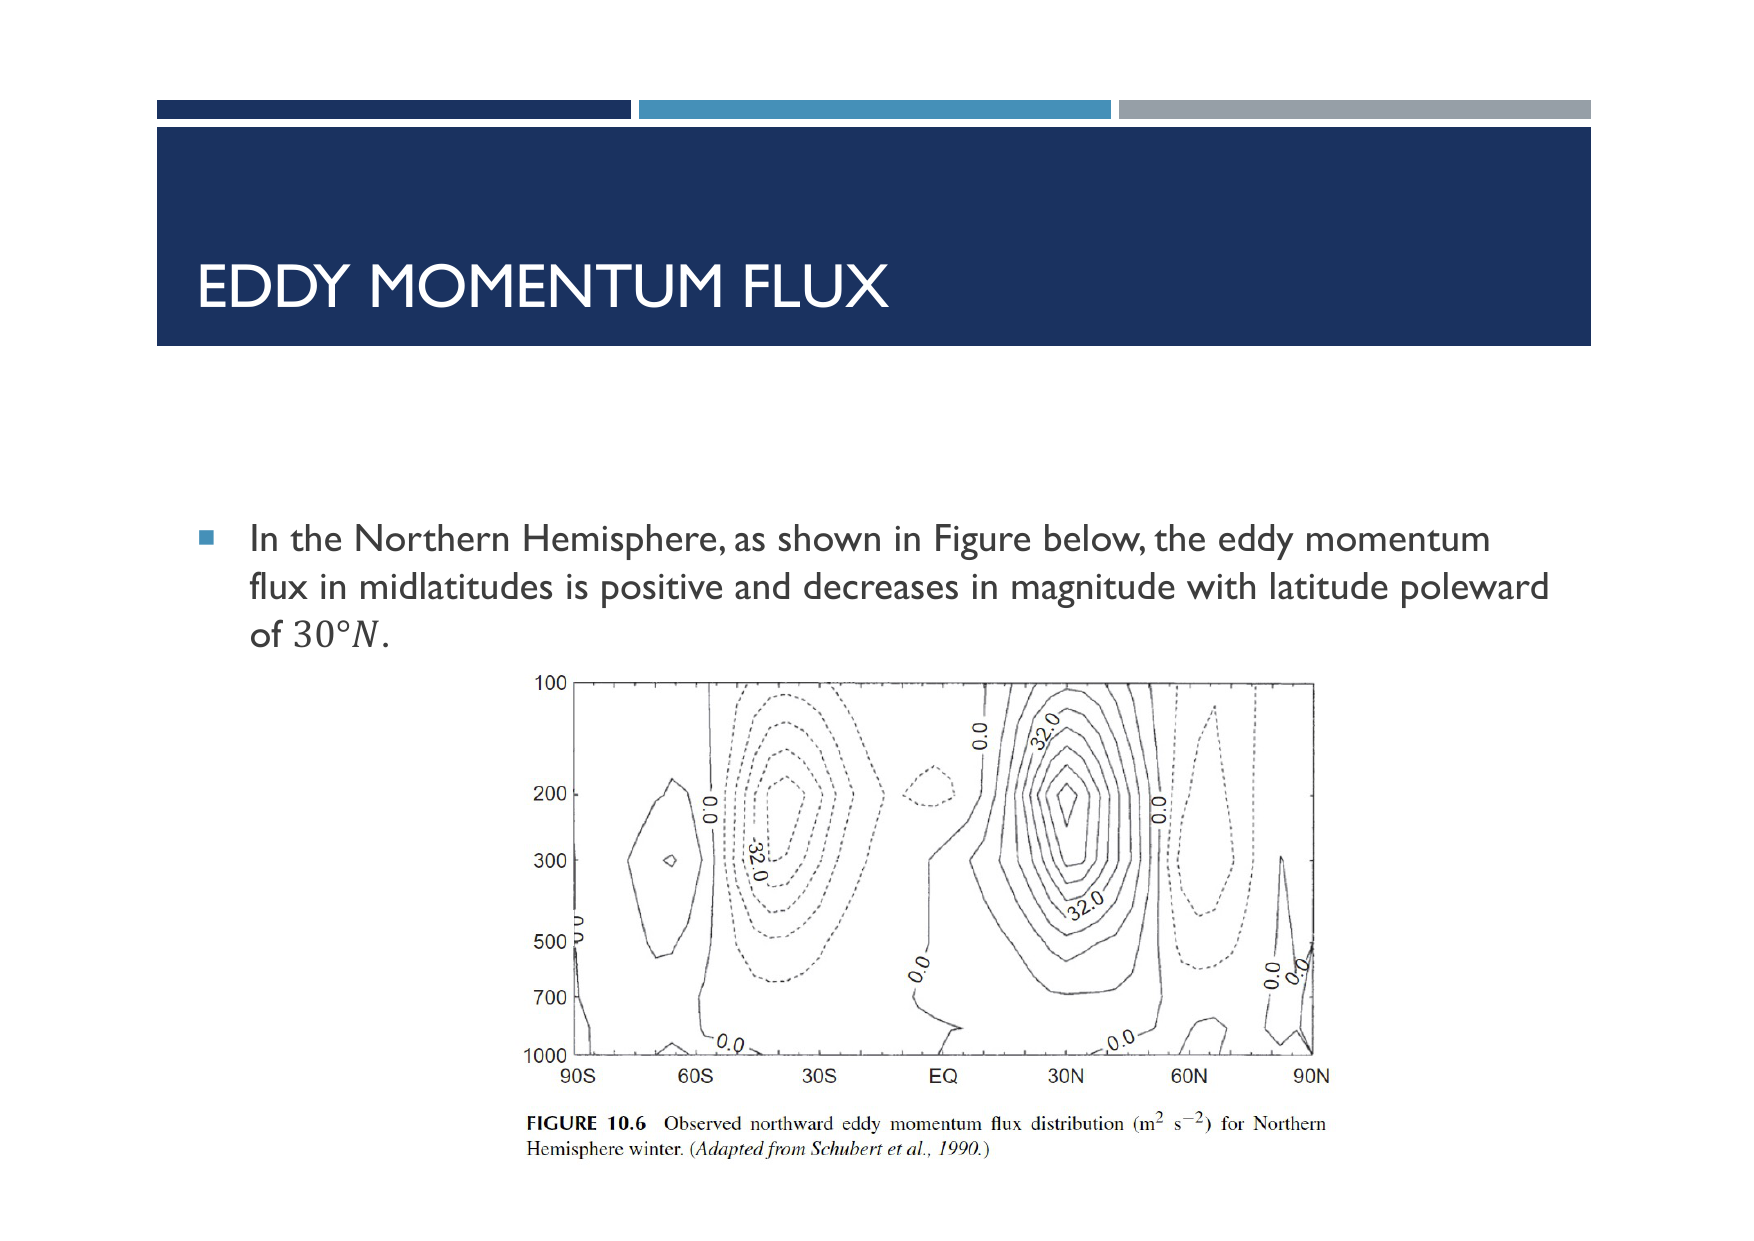
\includegraphics[width=0.85\textwidth]{images/ch07/p42_img01.png}
  \caption{Climatological zonal-mean eddy momentum flux $(u_E v_E)_Z$ in the
  Northern Hemisphere winter, plotted as a function of latitude (horizontal
  axis) and pressure (vertical axis).  Maximum values exceed
  $30$--$40$\,m$^2$\,s$^{-2}$ near $30$--$40^\circ$N at the $200$--$300$\,hPa
  level, coincident with the subtropical jet core.  Positive values throughout
  the midlatitude troposphere indicate persistent poleward (northward)
  transport of westerly momentum.
  \hisu{NH 겨울 $(u_E v_E)_Z$ 단면.  최댓값 30--40 m$^2$/s$^2$,
  위치 30--40$^\circ$N $\times$ 200--300 hPa --- 아열대 제트 코어 바로 옆.
  부호 양수 = 북쪽 (극 방향) 운동량 수송.}}
  \label{fig:ch07_trans_uv_cross}
\end{figure}

\begin{figure}[ht]
  \centering
  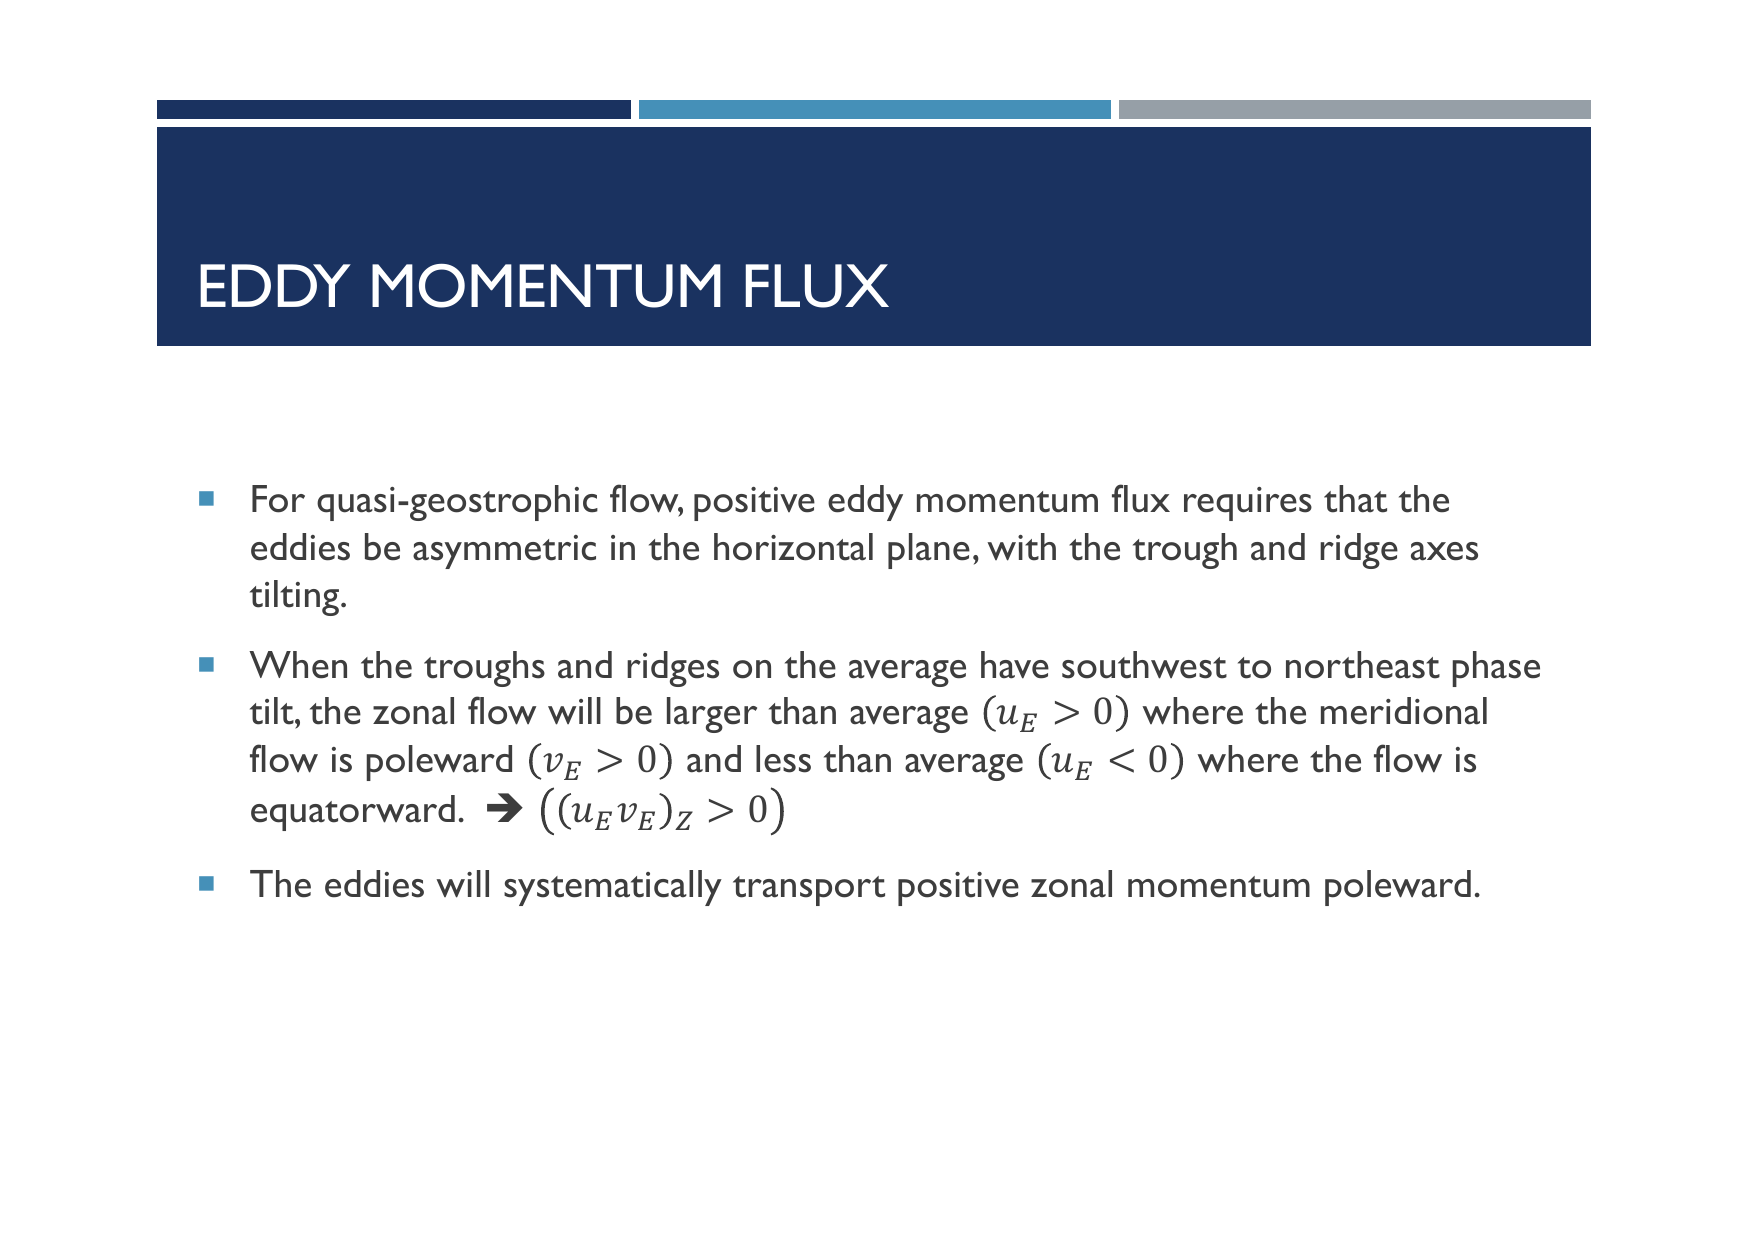
\includegraphics[width=0.85\textwidth]{images/ch07/p43_img01.png}
  \caption{Necessary condition for nonzero zonal-mean eddy momentum flux:
  the trough/ridge axes of Rossby waves must be \textbf{tilted} in the
  horizontal plane.  Shown are upper-tropospheric streamlines with SW--NE
  tilted trough axes in the NH (left) and NW--SE tilted axes in the SH
  (right).  This tilt yields $(u_E v_E)_Z > 0$ in NH and $(u_E v_E)_Z < 0$
  in SH — both consistent with \textit{poleward} (north in NH, south in SH)
  AM transport.
  \hisu{$(u_E v_E)_Z > 0$ 필요조건: trough axis가 NH에서 SW--NE 기울어짐.
  남반구에서는 NW--SE 기울어짐.  ``기울기 없으면 net flux 없음''.}}
  \label{fig:ch07_trans_qg_tilt}
\end{figure}

\eqref{eq:ch07_trans_eddy_approx}와 Figure~\ref{fig:ch07_trans_uv_cross}는
한 가지 사실을 분명히 한다: \textit{midlatitudes에서 long-term AAM 수송은
거의 전적으로 eddy flux로 결정된다}.  이것은 Ch.~4 §2.2에서 본 ``upgradient
momentum transport'' 관찰과 정확히 일치한다.

% --------------------------------------------------------------------------
\subsubsection{Quasi-Geostrophic Argument for Positive Eddy Flux}

왜 midlatitude eddy flux $(u_E v_E)_Z$가 \textit{체계적으로} 양수 (poleward)인가?
이 질문에 대한 정량적 답은 \textgr{quasi-geostrophic (QG) theory}로부터
얻어진다.  본 절에서는 직관적 논증을 두 단계로 제시한다.

\begin{figure}[ht]
  \centering
  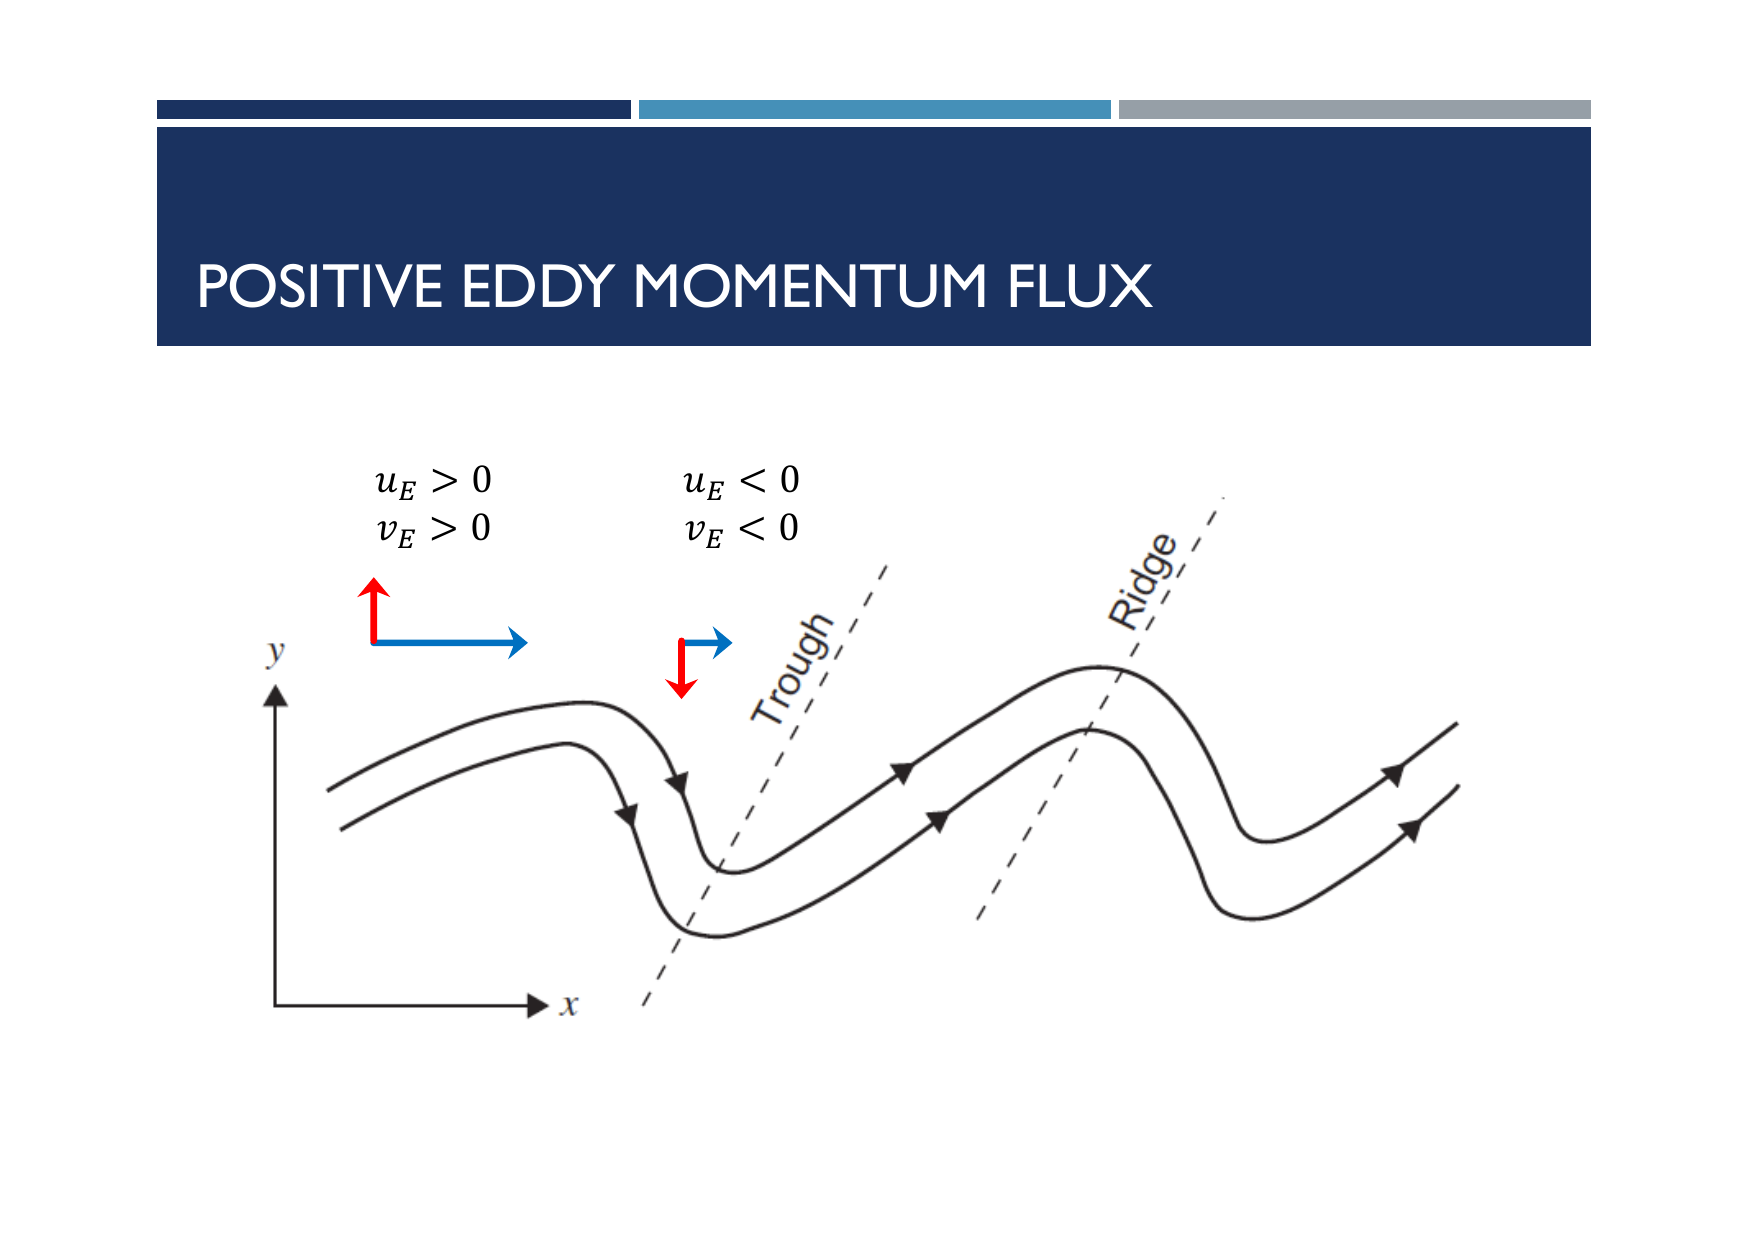
\includegraphics[width=0.85\textwidth]{images/ch07/p44_img01.png}
  \caption{Schematic of poleward eddy momentum transport in a midlatitude
  Rossby wave.  Air moving poleward (northward in NH) originates from lower
  latitudes where the climatological zonal-mean westerly is stronger; air
  moving equatorward originates from higher latitudes where westerlies are
  weaker.  Combined with a SW--NE trough tilt, the net result is a
  positive correlation $(u_E v_E)_Z > 0$ — i.e., northward transport of
  westerly angular momentum.
  \hisu{북쪽으로 가는 공기 = 더 강한 서풍 (큰 AM),
  남쪽으로 가는 공기 = 약한 서풍 (작은 AM) $\Rightarrow$ net 북쪽 AM 수송.
  trough가 SW--NE 기울어져 있어야 함.}}
  \label{fig:ch07_trans_qg_argument}
\end{figure}

\textbf{Step 1 — Tilt 조건.}  Ch.~4 §2.3의
Proposition~``Phase Condition for Nonzero Momentum Flux''에서 우리는 다음을
보았다:
\begin{equation}\label{eq:ch07_trans_tilt_condition}
   (u_E\,v_E)_Z > 0
   \;\;\Longleftrightarrow\;\;
   \text{NH에서 trough 축이 SW--NE로 기울어짐}.
\end{equation}
이 조건이 NH midlatitude Rossby wave에서 \textit{체계적으로 만족}된다는
사실은 관측에서 확인된다 (Figure~\ref{fig:ch07_trans_qg_tilt}).

\textbf{Step 2 — 왜 그 방향 tilt가 자연스러운가?}  Barocrinically 불안정한
중위도 jet은 ``downstream development'' 과정에서 점진적으로 동쪽으로 전파하는
wave packet을 만든다.  이 packet의 \textit{group velocity}는 mean flow의
$\beta$-effect에 의해 결정되며, energy conservation을 만족하려면 wave
ray가 자연스럽게 NH에서 SW--NE 방향을 향한다.  이는 \textgr{Rossby wave
dispersion}의 직접적 결과이다 (Holton \& Hakim 5th ed.\ Ch.~12.3).

\begin{theorem}[QG Argument for Poleward AM Transport]\label{thm:ch07_trans_qg_thm}
중위도 baroclinic Rossby wave는 다음 두 가지 효과의 결합으로 인해 자연스럽게
positive eddy momentum flux를 생성한다:
\begin{itemize}
  \item Poleward 이동하는 공기는 적도 쪽에서 출발 — 그 곳의 mean westerly
    $u_Z$가 더 강하므로 perturbation $u_E$가 양수 ($u' > 0$).
  \item Equatorward 이동하는 공기는 극 쪽에서 출발 — 그 곳의 $u_Z$가 더
    약하므로 $u' < 0$.
\end{itemize}
이 두 가지가 합쳐져 $(u_E v_E)_Z > 0$를 만든다.  Trough의 SW--NE tilt는
이 mechanism의 horizontal 표현이다.
\end{theorem}

\hisu{직관적 그림: ``남에서 북으로 가는 공기는 빠른 서풍을 가지고 오고,
북에서 남으로 가는 공기는 느린 서풍을 가지고 간다'' $\Rightarrow$ net 북쪽
서풍 AM 수송.}

\begin{hisublock}
이 \textgr{QG argument}는 운동량 수송의 \textit{upgradient} 성격을
설명하는 가장 명료한 논증이다.  순수한 ``diffusion'' 관점에서는 unstable한
현상으로 보이지만, 실제로는 (i) Rossby wave의 group velocity 구조와 (ii)
mean flow의 latitudinal shear $\partial u_Z/\partial \phi$가 만드는 phase
relationship으로부터 ``자연스럽게'' 양의 flux가 발생한다.  Pedlosky (1987)
Ch.~6의 \textit{Rossby wave energy} 논의를 보면 더 정확한 식
($k l < 0$ 조건이 NE 방향 group velocity와 SW--NE tilt에 해당)이 유도된다.
\end{hisublock}

% --------------------------------------------------------------------------
\subsubsection{Vertical Components of Momentum Flux Through the Surface}

위까지 다룬 것은 \textit{horizontal} (자오) momentum flux였다.  지표면을
가로지르는 \textit{vertical} momentum flux는 \eqref{eq:ch07_cons_threeterm}의
$\sigma = 1$ 경계 조건으로부터 나오며, 세 개의 별개 component로 분해된다:

\begin{align}
  \text{(i) Large-scale (mean) flux} :\;\; & \Omega a\cos\phi\,(p_s \dot\sigma)_Z,
     \label{eq:ch07_trans_vert_largescale} \\
  \text{(ii) Pressure (mountain) torque} :\;\; & a\cos\phi\,\Bigl(\sigma p_s
     \frac{\partial \Phi}{\partial x}\Bigr)_Z,
     \label{eq:ch07_trans_vert_pressure} \\
  \text{(iii) Turbulent stress} :\;\; & g a\cos\phi\,(\tau_E^z)_Z.
     \label{eq:ch07_trans_vert_turb}
\end{align}

\eqref{eq:ch07_trans_vert_largescale}는 surface mass flux ($\dot\sigma|_{\sigma=1}=0$
에 의해 사라지지만 그 직전 layer에서 nonzero일 수 있음)와 결합된 large-scale
AM 수송이고, \eqref{eq:ch07_trans_vert_pressure}는 \S3.1에서 본 mountain
torque이며, \eqref{eq:ch07_trans_vert_turb}는 \S3.2의 friction torque이다.

\begin{figure}[ht]
  \centering
  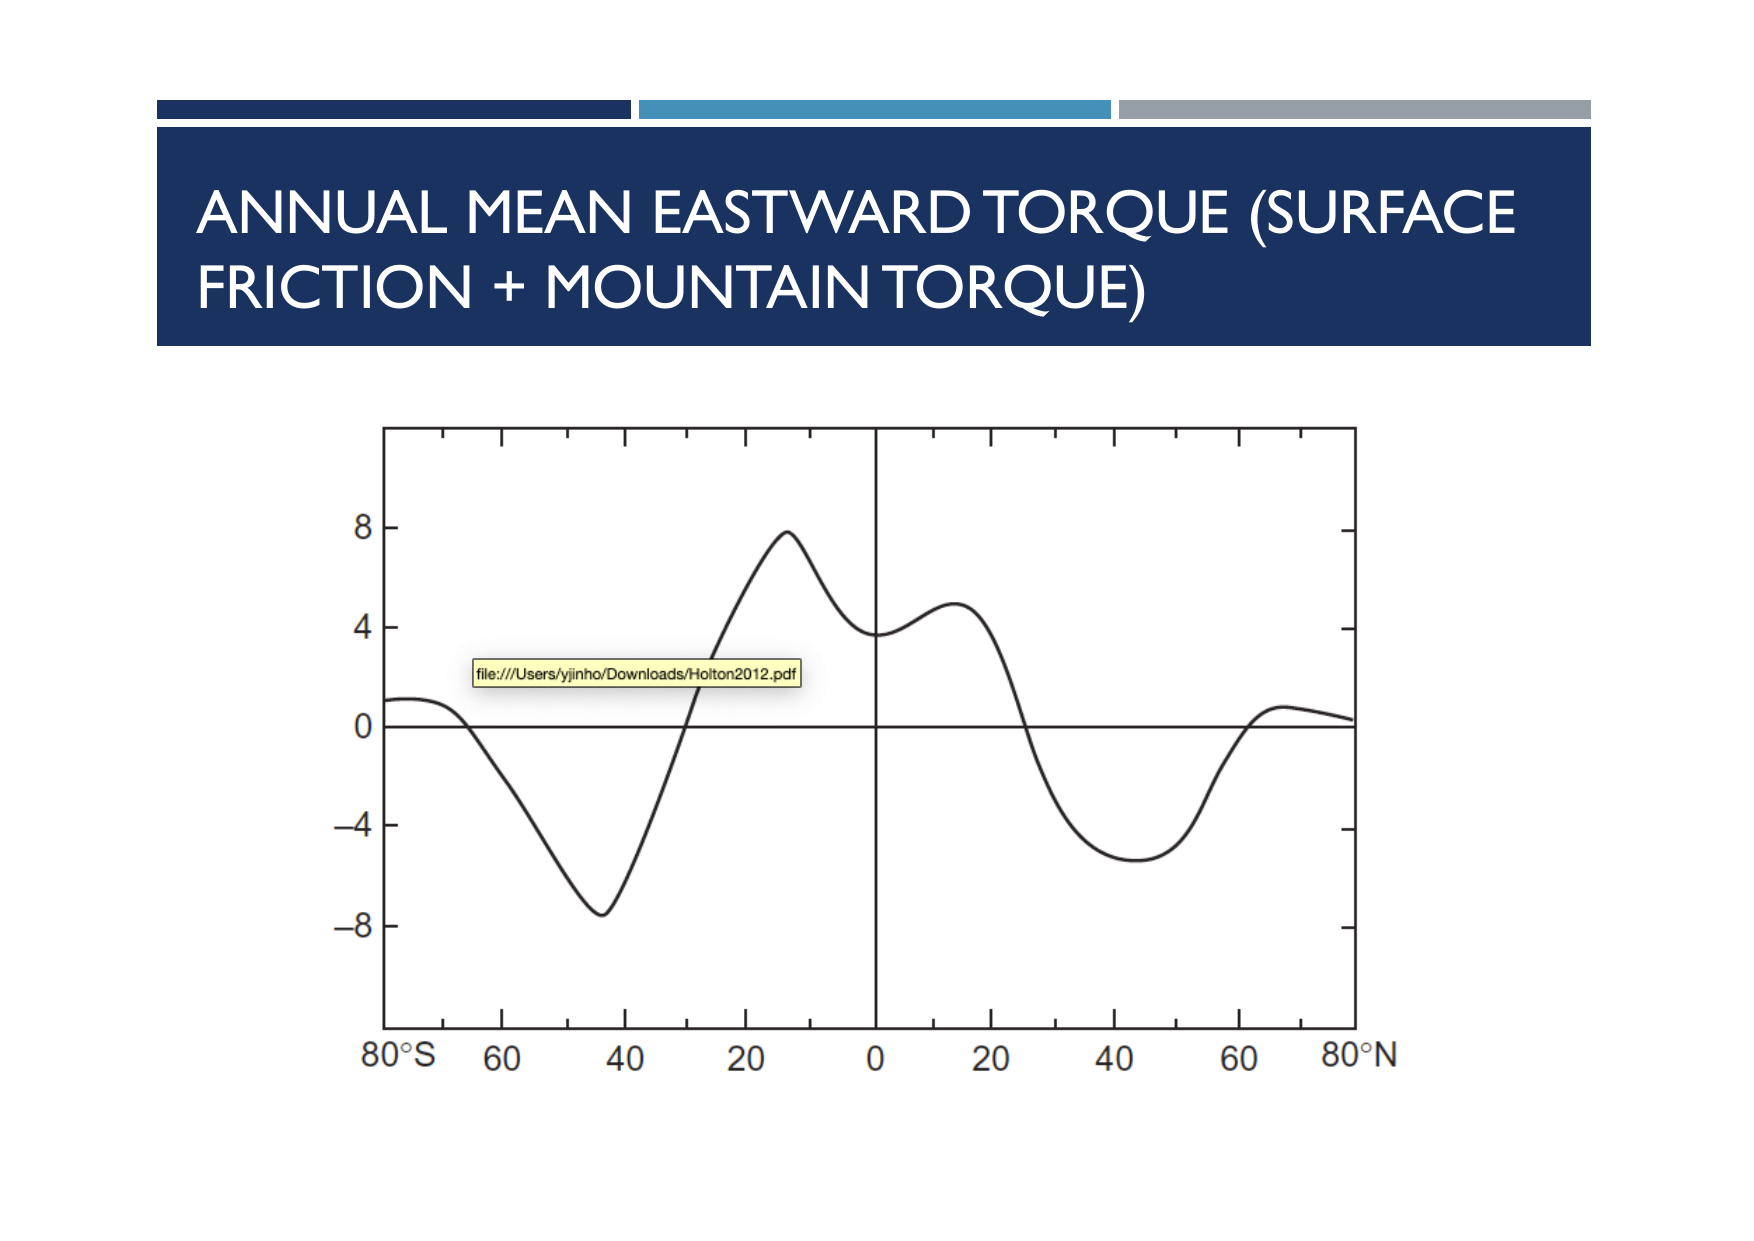
\includegraphics[width=0.85\textwidth]{images/ch07/p47_img01.png}
  \caption{Annual-mean eastward (zonal) torque per unit latitude at the
  Earth's surface, combining mountain torque and surface friction torque,
  plotted from $80^\circ$S to $80^\circ$N.  Positive values
  (atmosphere gains AM from Earth) occur within $\pm 20^\circ$ of the
  equator; negative values (atmosphere loses AM to Earth) dominate
  poleward of $20^\circ$ in both hemispheres.  Vertical scale $\pm 8$
  (arbitrary units).  This map confirms the source/sink structure
  underlying poleward AM transport.
  \hisu{지표 동방향 torque (마찰 + 산악) 연평균 분포.
  적도 $\pm 20^\circ$ 양수 (대기가 AM 얻음), 그 바깥은 음수 (대기가 AM 잃음).
  \S3와 \S4의 ``전체 그림''.}}
  \label{fig:ch07_trans_annual_torque}
\end{figure}

\eqref{eq:ch07_trans_vert_pressure}+\eqref{eq:ch07_trans_vert_turb}를 합친
``total eastward torque''의 latitudinal 분포는
Figure~\ref{fig:ch07_trans_annual_torque}와 같다:

\begin{itemize}
  \item \textbf{적도 $\pm 20^\circ$ 양수}: 대기가 지구로부터 westerly AM을 얻음.
    Easterly trade-wind belt에서의 friction torque가 지배적.
  \item \textbf{30--60$^\circ$ 음수}: 대기가 지구에 westerly AM을 잃음.
    Westerly 마찰 torque와 NH의 mountain torque가 합쳐진 결과.
  \item \textbf{극 부근 약한 양수}: 약한 polar easterly에 의한 양의 마찰 torque.
\end{itemize}

\hisu{한 그림에 담긴 \S3의 모든 내용 — ``남북 단면으로 보는 대기-지구 AM
수지''.}

% --------------------------------------------------------------------------
\subsubsection{Observational Confirmation: Eddy Flux Dominance Outside the Deep Tropics}

마지막으로 우리는 관측 자료가 \textit{drift vs.\ eddy} 분할
\eqref{eq:ch07_trans_three_flux}을 어떻게 확인하는지 본다.

\begin{figure}[ht]
  \centering
  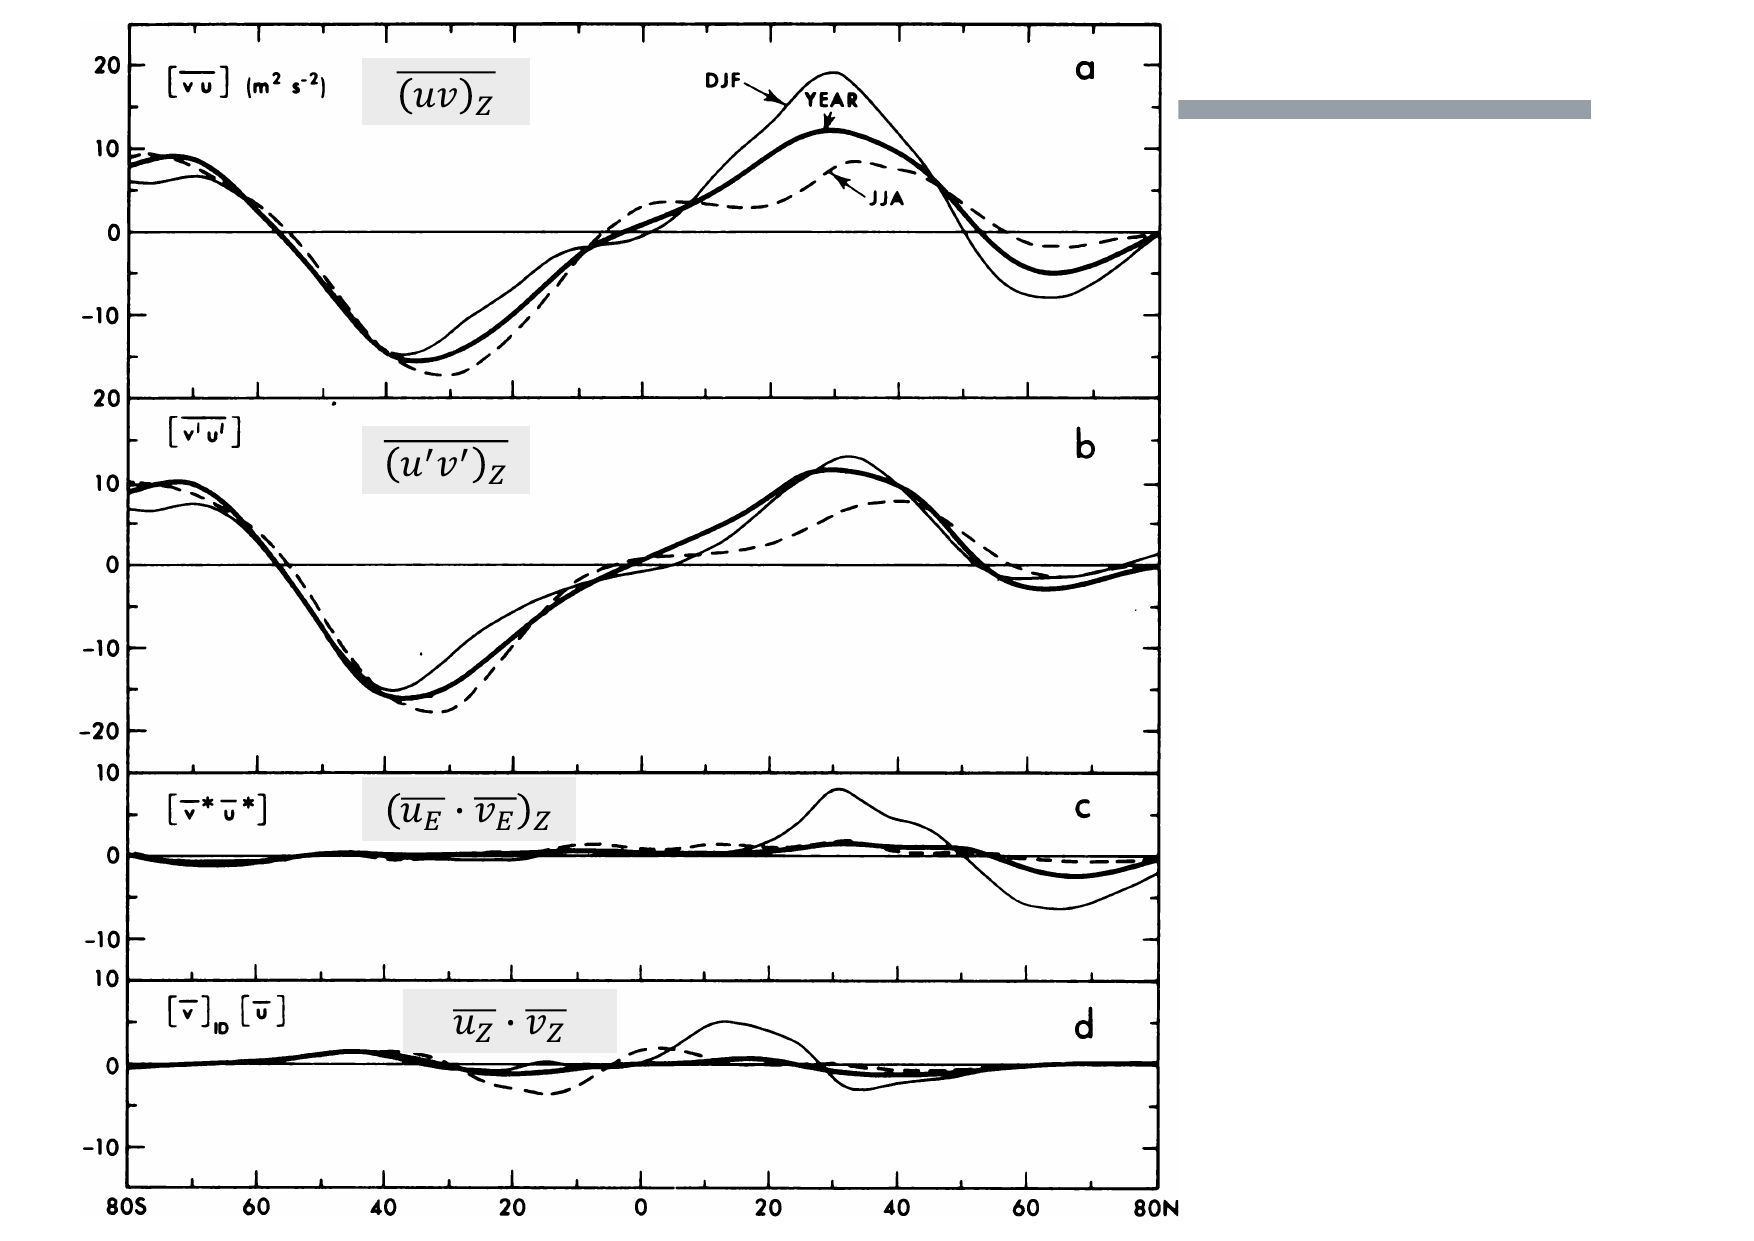
\includegraphics[width=0.85\textwidth]{images/ch07/p49_img01.png}
  \caption{Four-panel decomposition of the vertically integrated meridional
  angular momentum flux across each latitude, separated into DJF, JJA, and
  annual (YEAR) means.  Panel (a) shows $[\bar v\bar v]$ (zonal mean
  meridional advection of zonal-mean momentum), (b) $(\overline{u'v'})_Z$
  (transient eddy flux), (c) $[\bar u^*\bar v^*]$ (stationary eddy flux),
  and (d) $[\bar v]_{10}[\bar u]$ (combined mean meridional + zonal-mean
  zonal wind product).  Outside $\pm 10^\circ$ of the equator, the
  transient eddy flux (b) dominates all other contributions.
  \hisu{4-panel 분해: (a) 평균 $\bar v\bar v$, (b) transient eddy
  $\overline{u'v'}$, (c) stationary eddy $\bar u^*\bar v^*$, (d) drift.
  적도 $\pm 10^\circ$ 밖에서는 거의 모든 flux가 transient eddy (b)에서
  나옴.}}
  \label{fig:ch07_trans_four_panel}
\end{figure}

Figure~\ref{fig:ch07_trans_four_panel}의 4-panel 분해에서 보이는 핵심
결과는 다음과 같다:

\begin{theorem}[Eddy Flux Dominance]\label{thm:ch07_trans_eddy_dominance}
적도 양쪽 $\pm 10^\circ$ 영역 밖의 모든 위도에서, 자오 AAM flux는 거의
전적으로 transient (+ small stationary) eddy flux $(u_E v_E)_Z$에 의해
결정된다.  Mean drift flux $u_Z (p_s v)_Z$는 deep tropics (Hadley cell
upper branch)에서만 의미 있는 기여를 한다.
\end{theorem}

\hisu{관측 결론: 적도 ±10$^\circ$ 밖은 eddy가 \textbf{거의 전부}.
열대만 mean drift (Hadley cell)가 함께 작용.}

\begin{remark}[Why This Matters for Climate Models]\label{rem:ch07_trans_models}
이 결과는 GCM의 격자 해상도가 \textit{transient eddy}를 충분히 분해해야
한다는 강력한 요청이다.  Eddy를 cumulus-style parameterize한다는 시도는
heat flux는 어느 정도 흉내낼 수 있지만 \textit{upgradient} momentum flux는
재현하지 못한다.  현실의 GCM은 모두 explicit eddy resolution (수평
$\sim$100\,km 이하)을 채택한다.
\end{remark}

\begin{hisublock}
\textbf{\S4 종합}:
\begin{enumerate}
  \item 표면 wind 분포 (열대 east, 중위도 west)가 두 source/sink 영역 형성.
  \item Stationarity가 source→sink poleward AAM transport를 강제.
  \item Long-term 균형은 \eqref{eq:ch07_trans_two_term} 두 항으로 닫힘.
  \item Meridional AAM flux는 3항 분해 $\to$ solid 항 자동 0 (mass 보존),
    drift는 열대, eddy는 중위도 지배.
  \item QG argument: trough의 SW--NE tilt + Rossby wave dispersion →
    체계적 positive $(u_E v_E)_Z$ → 극방향 운동량 수송.
  \item 관측 4-panel 분해에서 적도 ±10$^\circ$ 밖 거의 모든 flux는 transient
    eddy로부터 옴.
\end{enumerate}

\medskip
\textbf{\S5로의 연결}: 지금까지 본 것은 모두 \textit{시간 평균} balance이다.
다음 절 \S5에서는 이 balance의 \textbf{시간 변동}성 — 일별, 계절, 수년
시간 규모에서의 AAM 변화 — 을 LOD 측정 및 산악/마찰 torque 시계열과 함께
검토한다.
\end{hisublock}
% =============================================================================
%   SECTION 5 — Temporal Variations in AAM
% =============================================================================

\subsection{Temporal Variations in AAM}

지금까지의 논의는 모두 \textbf{long-term annual mean}의 균형 구조에 초점을 맞추었다.
즉 tropics에서 friction torque로 atmosphere가 AM을 얻고, mid-latitudes에서
mountain + friction torque로 AM을 잃으며, 그 사이를 eddy-driven poleward
flux가 연결한다는 \emph{steady-state} 그림이었다.  그러나 실제 대기에서는
이 평형이 \textbf{시간에 따라 끊임없이 동요}하며, 그 fluctuation 자체가
AM budget의 물리를 가장 선명하게 드러낸다.

이 절에서는 (i) \textgr{monthly time scale}에서 LOD와 atmospheric AM의 정확한
1:1 대응, (ii) \textgr{daily time scale}에서 torque-tendency balance의 강한
변동성, (iii) pressure torque의 \textgr{spatial preferred pattern}, 그리고
(iv) 모든 것을 통합한 \textgr{MMC-eddy-friction 4-point closure}를 살펴본다.

\hisu{핵심 질문 --- AAM은 왜 시간에 따라 변하는가? 그리고 그 변동을 만들어내는
\textbf{torque}와 \textbf{eddy flux}는 어떤 시간 척도에서 각각 지배적인가?}


% --------------------------------------------------------------------------
\subsubsection{Monthly AAM Time Series: LOD-AAM Correspondence}

가장 거시적인 관측 사실부터 출발하자.  지구의 \textgr{length of day} (LOD)는
초정밀 천문/측지 (VLBI, GPS) 측정으로 $10^{-5}$ s 수준에서 monitoring되며,
한편 \textgr{atmospheric angular momentum} (AAM)은 reanalysis 풍 자료로부터
$M = \Omega R^2\cos^2\phi + uR\cos\phi$의 부피 적분으로 독립적으로 산출된다.
이 두 양은 본래 전혀 다른 measurement chain에서 나오지만, 다음의 보존 법칙으로
연결된다.

\begin{equation}\label{eq:ch07_temp_lod_aam}
  M_{\text{Earth}} + M_{\text{atm}} + M_{\text{ocean}} + M_{\text{core}}
    = \text{const.}
\end{equation}

\hisu{지구계 전체 AM 보존: 대기 AM이 증가하면 그만큼 지각/맨틀 AM이 감소
($\Rightarrow$ LOD 증가, 즉 지구 자전 감속).}

\begin{remark}[Why does LOD respond to AAM?]
지구 자전 AM은 $M_{\text{Earth}} = I\Omega_E$ ($I$: moment of inertia,
$\Omega_E$: rotation rate)이다.  $I$가 거의 일정하므로
$\Delta M_{\text{Earth}} = I\Delta\Omega_E$이며, 한편 LOD는
$\text{LOD} = 2\pi/\Omega_E$이므로
\begin{equation}\label{eq:ch07_temp_dlod}
  \frac{\Delta \text{LOD}}{\text{LOD}} = -\frac{\Delta\Omega_E}{\Omega_E}
    = \frac{\Delta M_{\text{atm}}}{I\Omega_E}.
\end{equation}
대기-해양-코어 중 \textbf{decadal보다 짧은} 시간 척도에서 LOD 변동의
지배 원인은 거의 전적으로 \emph{atmosphere}이다 (ocean $\lesssim$5\%,
core: decadal 이상에서만 유의).
\end{remark}

\hisu{LOD가 길어졌다 = 지구가 천천히 돈다 = 그만큼 AM이 어디론가 갔다.
계절-연 단위에서 그 "어디론가"는 거의 100\% 대기다.}


\begin{figure}[htbp]
  \centering
  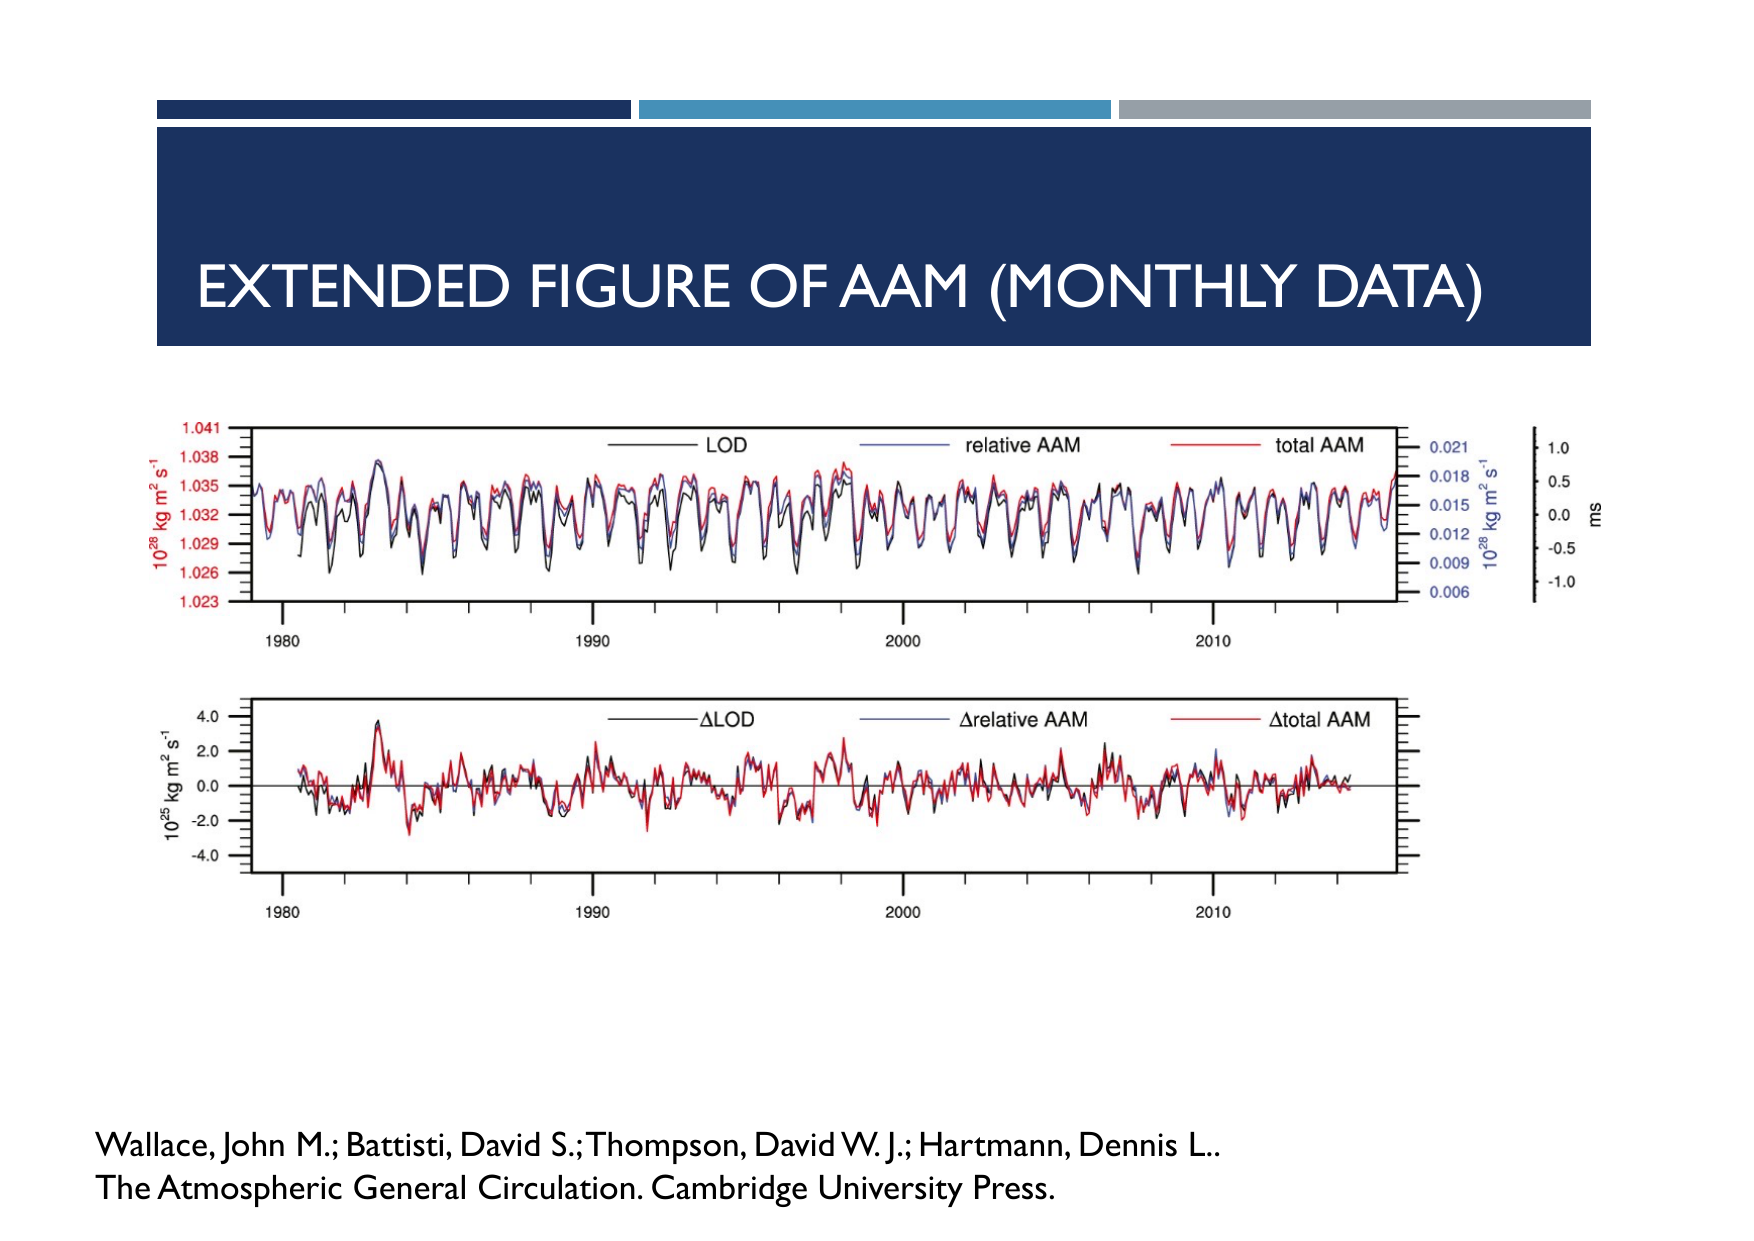
\includegraphics[width=0.85\textwidth]{images/ch07/p51_img01.png}
  \caption{Monthly time series (1980--2020) of length-of-day (LOD, top), relative
  atmospheric angular momentum $M_r$ (middle), and total atmospheric AM
  $M = M_\Omega + M_r$ (bottom), with the lower panel showing the corresponding
  monthly tendencies $\Delta\text{LOD}$, $\Delta M_r$, $\Delta M$.  The three
  series are virtually identical after sign convention --- a remarkable
  observational confirmation that the Earth-atmosphere system is angular-momentum
  closed on monthly time scales. \hisu{LOD, 상대 AAM, 총 AAM 세 곡선이
  거의 완전히 일치한다는 사실은, 풍 자료와 천문 자료라는 두 독립 채널이
  같은 보존 법칙을 만족함을 보여준다 --- 곧 대기-지구계가 \emph{closed system}
  이라는 결정적 증거다.}}
  \label{fig:ch07_temp_monthly_lod_aam}
\end{figure}


\medskip



\noindent\textbf{Three series are virtually identical.}
Figure~\ref{fig:ch07_temp_monthly_lod_aam}에서 가장 중요한 관측은 LOD,
relative AAM, total AAM이 거의 \textbf{똑같은 곡선}이라는 점이다.  이는 다음
두 사실을 동시에 함의한다.

\begin{enumerate}
  \item \textbf{Total AAM이 relative AAM 변동에 의해 지배된다.}
    $M_\Omega = \Omega R^2\cos^2\phi$ 부분은 시간 변동이 없으므로
    ($\Omega$, $R$, $\phi$ 모두 고정), $\Delta M_{\text{atm}}$의 본체는
    오로지 $\Delta M_r$, 즉 \emph{wind anomaly}이다.  곧 LOD 변동을 만드는
    물리적 주체는 \textgr{zonal wind anomaly}이다.

  \item \textbf{Closed system 가설의 관측적 검증.}
    LOD (천문)와 AAM (풍)이 1:1로 일치한다는 것은 \eqref{eq:ch07_temp_lod_aam}의
    가정 (해양/코어 효과 무시)이 monthly scale에서 매우 정확함을 뜻한다.
\end{enumerate}


\medskip



\noindent\textbf{Seasonal cycle: boreal summer dip.}
계절 곡선을 자세히 보면, 매년 \textbf{boreal summer} (6--8월) 부근에 뚜렷한
$M$의 minimum이 나타나고, 겨울 (12--2월)에 maximum이 위치한다.  진폭은
$\sim 2\times 10^{25}$ kg m$^2$ s$^{-1}$ 수준으로, 표준 편차의 약 2배다.

이 계절성의 물리적 원인은 두 가지다.

\begin{itemize}
  \item \textgr{Tibetan anticyclone}: 보리얼 여름철 티벳 고원 상공에 대형
    상층 anticyclone이 발달하면, 그 남쪽 가장자리에 강한 \emph{easterly}가
    형성된다 (TEJ, Tropical Easterly Jet).  Easterly는 $u < 0$이므로
    $M_r$ 감소.
  \item \textgr{Westerly jet의 북상}: 여름철 NH 중위도 jet이 50--60$^\circ$N로
    북상하면서, AM 가중치 $a\cos\phi$가 작은 위도대로 이동.  같은 $u$라도
    $M_r = u a\cos\phi$가 줄어든다.
\end{itemize}

\hisu{여름철 $M_r$ 감소 = (1) TEJ가 적도부 westerly를 easterly로 바꾸어
$M_r$을 끌어내리고, (2) NH 중위도 jet이 북상하면서 적도 가까이의 큰 가중치
영역에서 westerly가 빠져나간다.  이 두 효과가 합쳐져 boreal summer dip을
만든다.}


\begin{hisublock}
\textbf{Peixoto \& Oort (1992) Ch.~11과의 비교.}  Peixoto \& Oort,
\textit{Physics of Climate}, Ch.~11 (특히 Figs.~11.5--11.6)에서 동일한
LOD-AAM correspondence가 1976--1988년 자료로 제시되어 있으며, 본 책의
Fig.~\ref{fig:ch07_temp_monthly_lod_aam} (1980--2020)는 그 결과의 거의 4배에
달하는 장기 관측 기간에서 동일한 결론을 재확인한다.  특히 ENSO 관련 양/음
편차 (1982/83, 1997/98, 2015/16 El Ni\~no 해의 양의 AAM anomaly)가 명확히
보이며, 이는 적도 태평양 SST가 Hadley cell 강도 → westerly anomaly →
$M_r$ 증가의 사슬로 LOD에 즉시 신호를 남김을 보여준다.  Rosen et al. (1990,
\textit{J.\ Geophys.\ Res.}, 95, 265--275) 또한 ENSO와 LOD의 lag 1--2 month
관계를 정량화하였다.
\end{hisublock}


% --------------------------------------------------------------------------
\subsubsection{Daily Variability: Torque vs.\ Tendency}

Monthly scale에서는 LOD와 AAM이 깔끔히 일치했지만, \textgr{daily} scale로
내려가면 훨씬 격렬한 변동이 드러난다.  이 변동의 주체는 더 이상 천천히
변하는 jet 위치가 아니라, \textbf{매일의 surface torque} 자체다.

전체 대기에 대해 \eqref{eq:ch07_temp_lod_aam}을 시간 미분하면

\begin{equation}\label{eq:ch07_temp_tendency_torque}
  \frac{dM_{\text{atm}}}{dt} = \mathcal{T}_{\text{press}}
    + \mathcal{T}_{\text{fric}} + \mathcal{T}_{\text{gw}},
\end{equation}

\noindent
좌변은 AAM \textgr{tendency}, 우변은 mountain (pressure), frictional, gravity-wave
torque의 합이다.  Daily 자료에서는 좌변과 우변의 일치 정도를 직접 검증할 수 있다.


\begin{figure}[htbp]
  \centering
  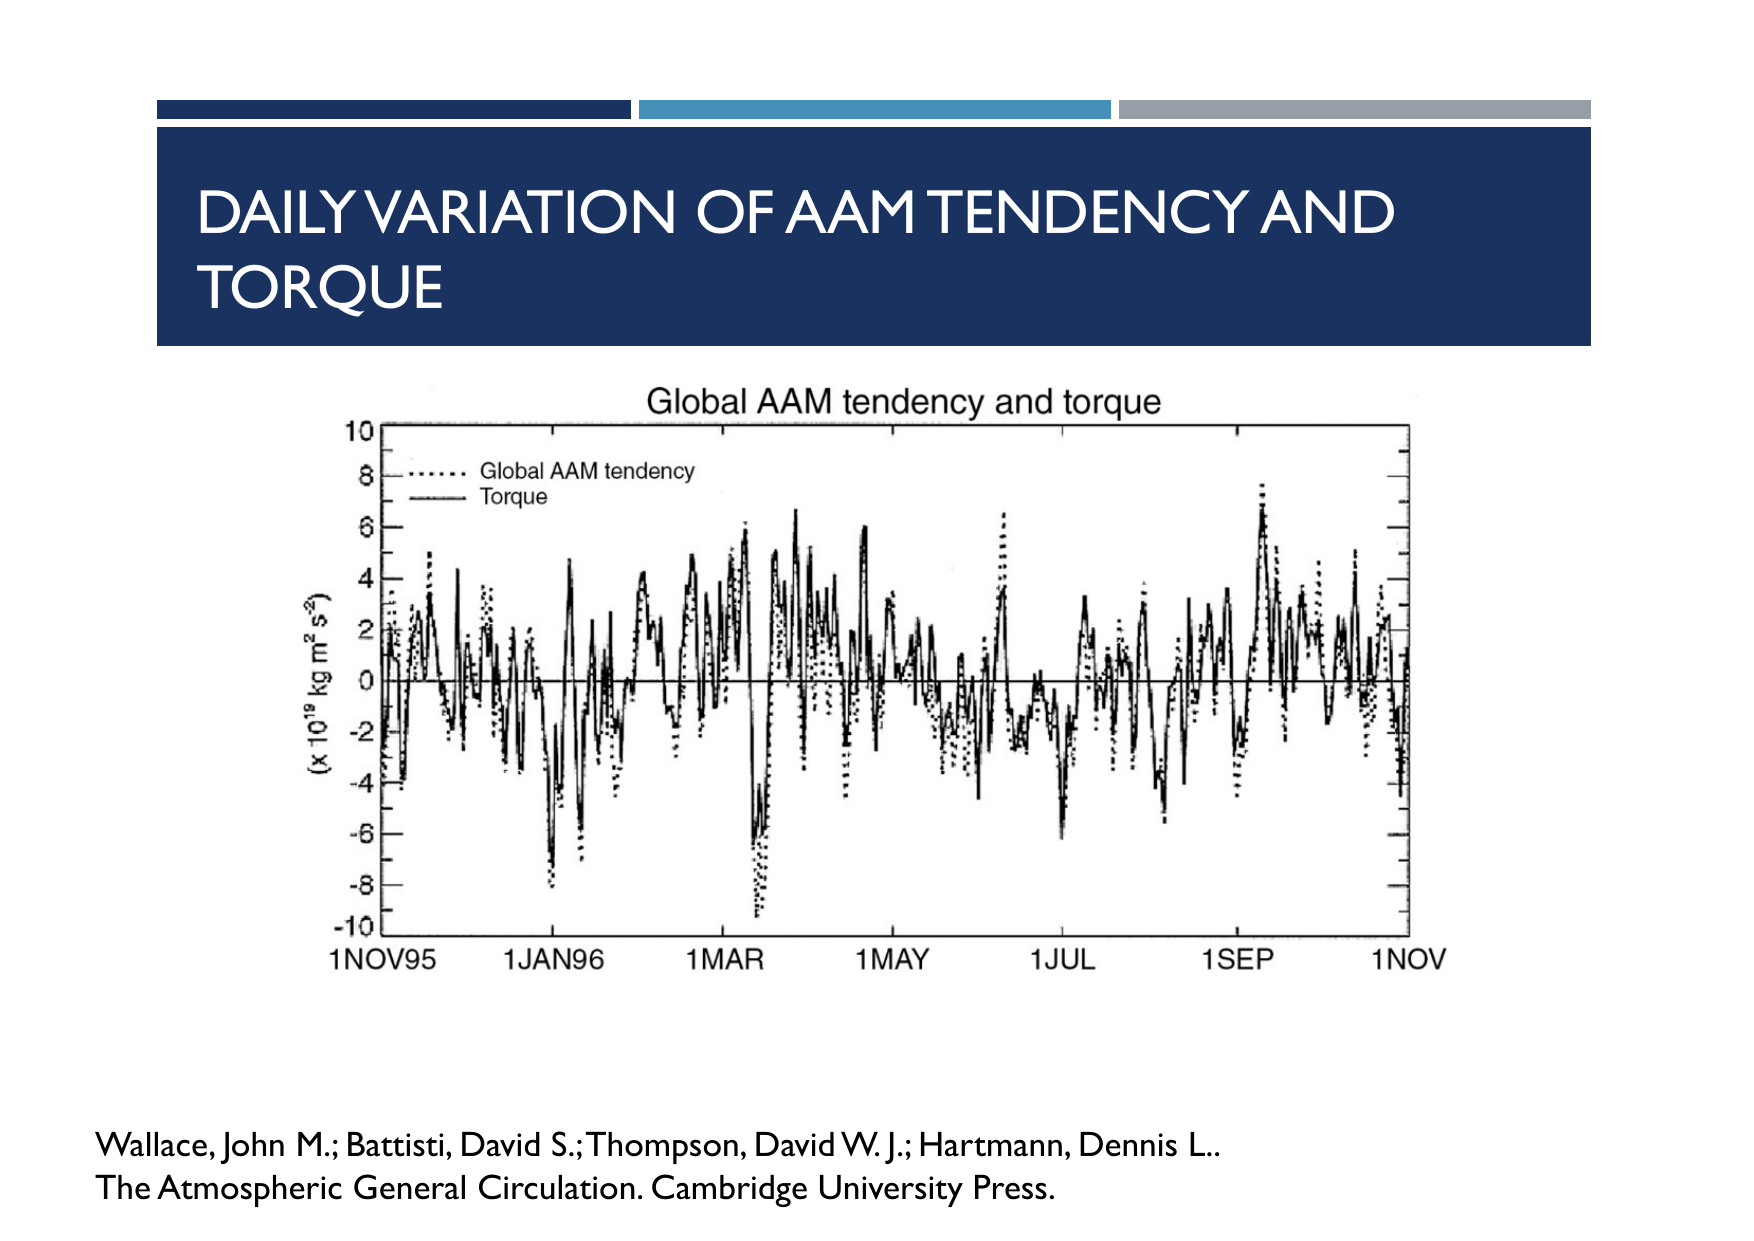
\includegraphics[width=0.85\textwidth]{images/ch07/p53_img01.png}
  \caption{Daily time series (1 Nov 1995 -- 1 Nov 1996) of global atmospheric AAM
  tendency $dM/dt$ (dashed) and total surface torque
  $\mathcal{T}_{\text{press}}+\mathcal{T}_{\text{fric}}$ (solid), in units of
  $10^{19}$ kg m$^2$ s$^{-2}$.  Both curves oscillate within
  $\pm 6\text{--}8\times 10^{-3}$ kg m$^2$ s$^{-2}$ (rescaled per unit mass)
  and track each other closely, demonstrating that day-to-day AAM changes are
  driven by the day-to-day surface torque. \hisu{매일의 AAM 변동량과 surface
  torque가 거의 함께 움직인다 --- 대기 AAM은 \emph{torque에 의해 직접 끌려가는}
  양이지, eddy flux convergence에 의한 위도별 redistribution만으로 설명되지
  않는다 (eddy는 위도 간 transfer를 일으킬 뿐 global AAM에는 기여 못함).}}
  \label{fig:ch07_temp_daily}
\end{figure}


\medskip



\noindent\textbf{Variability amplitude.}
Figure~\ref{fig:ch07_temp_daily}의 두 곡선은 모두 $\pm 6\text{--}8\times 10^{-3}$
kg m$^2$ s$^{-2}$ 범위에서 oscillate한다 (단위 질량당 표기, global AAM 자체로는
$10^{19}$ 단위).  이 변동폭은 monthly mean 자체보다도 큰 값으로, daily
fluctuation이 결코 작은 noise가 아님을 보여준다.  \emph{Synoptic} 시간
척도에서 individual storm systems가 mountain ridge 위로 통과할 때마다,
그리고 boundary-layer friction이 계절 내 변동을 보일 때마다, 곧바로 atmospheric
AAM 신호가 발생한다.


\medskip



\noindent\textbf{Torque decomposition.}
Daily torque는 두 성분으로 나뉜다.

\begin{equation}\label{eq:ch07_temp_torque_decomp}
  \mathcal{T}_{\text{press}}(t) = -\oint a\cos\phi\,
    \left(p_s\frac{\partial h}{\partial x}\right)_Z d\phi,\qquad
  \mathcal{T}_{\text{fric}}(t) = -\oint a\cos\phi\,
    (\tau_E^x)_Z\big|_{\sigma=1}\, d\phi.
\end{equation}

\hisu{각각은 §3에서 정의한 mountain torque (산악 동서 SLP 차)와 friction torque
(지표 동서 stress)를 global하게 적분한 것이다.  Daily scale에서는 두 항이
\emph{같은 정도}로 변동하며, 어느 한쪽도 지배적이지 않다.}


\medskip



\noindent\textbf{Pre-1990s data quality issues.}
1990년대 이전의 reanalysis는 (i) 산악 미분석 (orographic detail 부족),
(ii) 거친 boundary-layer parameterization, (iii) 위성 자료 부재로 인한 SH
관측 부족 등의 이유로 daily torque-tendency balance가 \textbf{덜 정확}했다.
ECMWF ERA-40 이후, 특히 ERA-Interim 및 ERA5 (2010s)에서는 이 일치도가
극적으로 향상되었다.  Egger \& Hoinka (1999, \textit{J.\ Atmos.\ Sci.},
56, 1305--1313)는 NCEP/NCAR reanalysis의 1994--1996 4년치 일자료에 대해
torque-tendency 상관계수를 산출한 결과 $r\approx 0.86$을 보고하였다.

\begin{remark}[Why $r \neq 1$?]
완벽한 closure ($r=1$)가 달성되지 않는 이유는 (i) \textgr{gravity-wave drag}
torque가 reanalysis output에 명시적으로 포함되지 않을 수 있고, (ii) friction
stress 자체가 parameterized된 양이며, (iii) AAM tendency는 24시간 차분에
의해 다소 거친 추정치라는 데 있다.  $r\approx 0.86$이라는 값은 그러나
\eqref{eq:ch07_temp_tendency_torque}의 물리가 daily scale에서도 \emph{잘
성립함}을 보여주기에 충분히 높은 수치다.
\end{remark}


% --------------------------------------------------------------------------
\subsubsection{Spatial Pattern of Pressure Torque}

Daily torque-tendency balance가 잘 성립한다는 것은 알겠지만, 그 \emph{공간
구조}는 어떠한가?  특히 mountain torque는 본질적으로 \textgr{regional} 양으로,
어떤 산맥의 어느 쪽 사면에서 SLP anomaly가 발달했느냐에 따라 부호가 결정된다.

이를 정량적으로 보기 위해 다음의 \textgr{regression analysis}를 수행한다.
Global mean AAM tendency $dM/dt$를 predictor로 삼아, 각 격자점의 SLP를
회귀시킨다.

\begin{equation}\label{eq:ch07_temp_regression}
  \text{SLP}(x,y,t) \sim \beta(x,y)\,\frac{dM}{dt}(t) + \text{residual}.
\end{equation}

\hisu{$\beta(x,y)$의 공간 분포는 "AAM이 증가하는 날 어디의 SLP가 평균적으로
더 높은가" 라는 \emph{associated pattern}을 시각화한다.}


\begin{figure}[htbp]
  \centering
  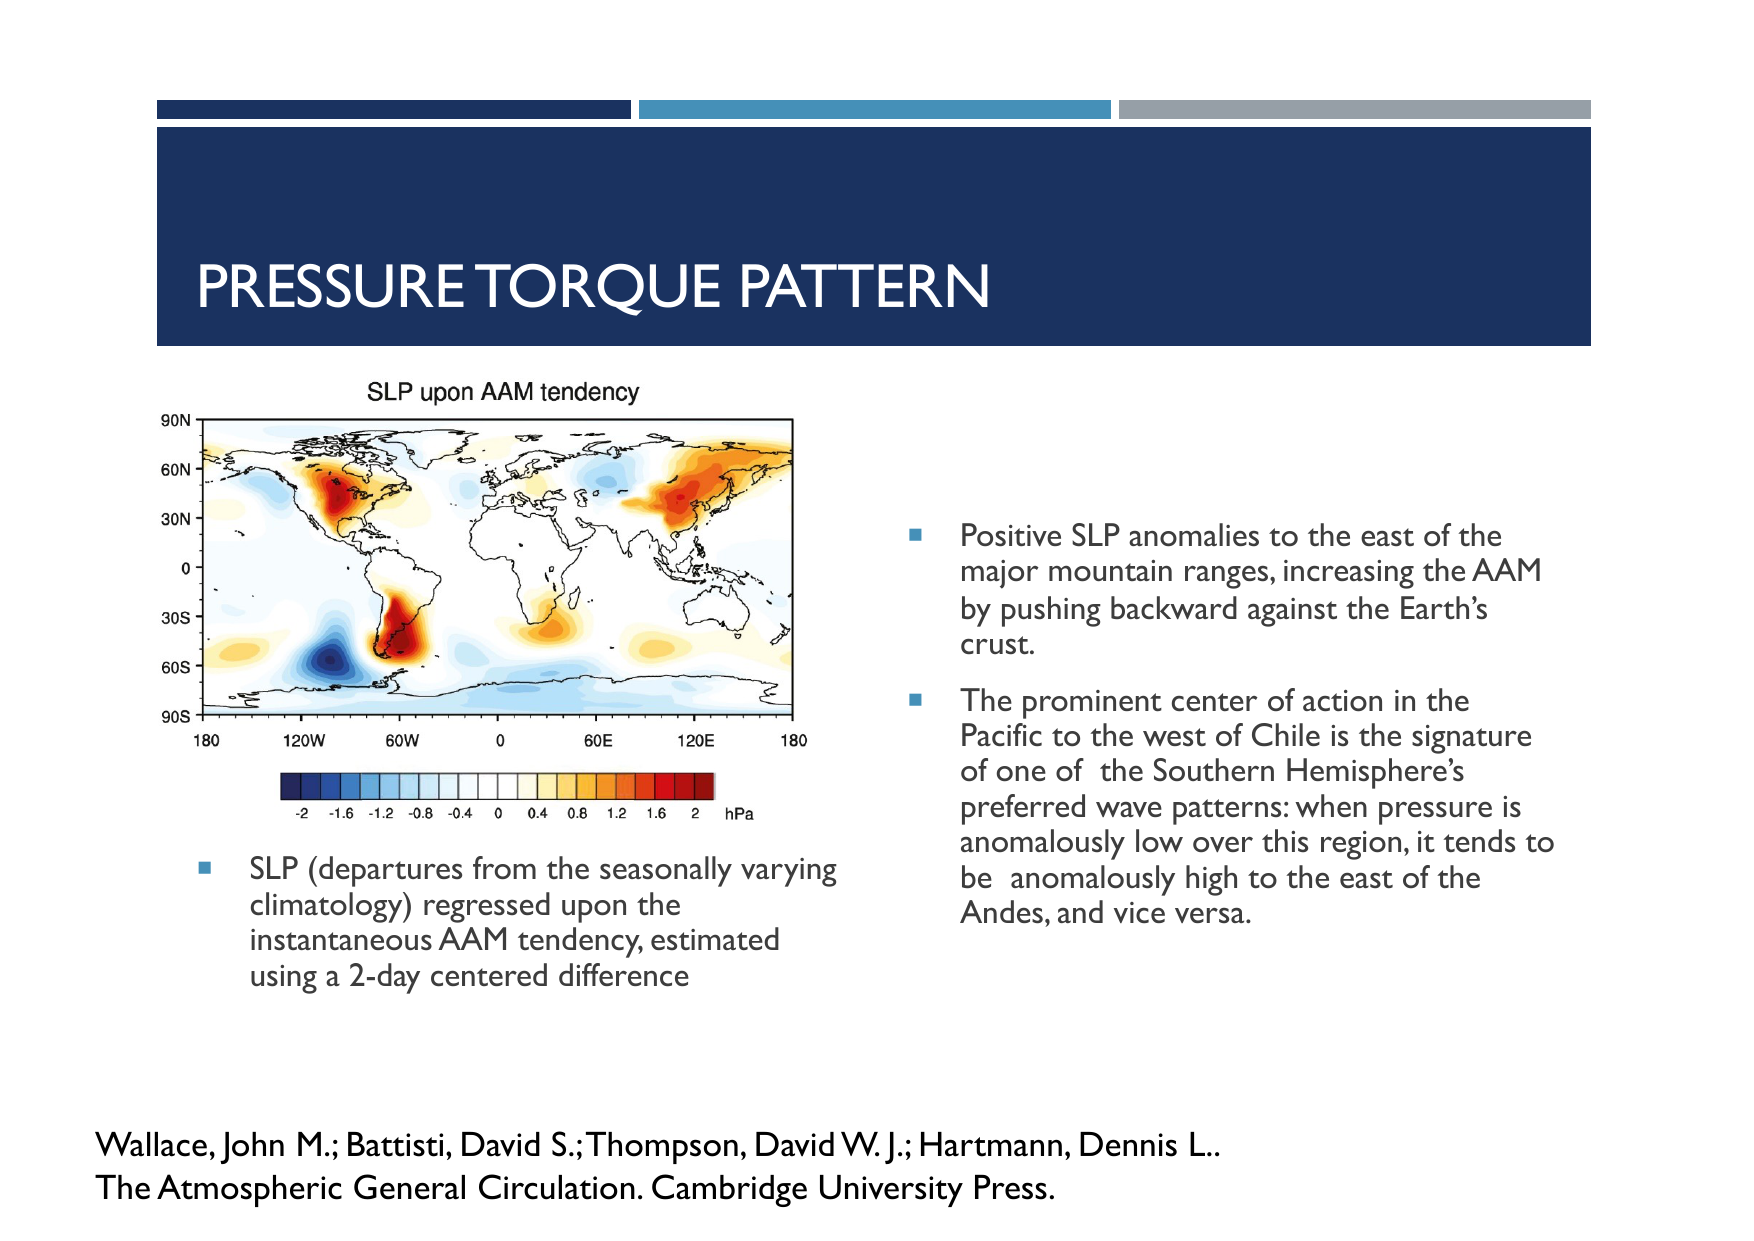
\includegraphics[width=0.85\textwidth]{images/ch07/p55_img01.png}
  \caption{Regression of sea-level pressure (SLP) anomalies onto the global
  AAM tendency $dM/dt$.  Positive (negative) regression values indicate higher
  (lower) SLP on days when atmospheric AAM is increasing.  The dominant feature
  is a positive SLP anomaly on the eastern flank of major mountain ranges ---
  most strikingly the South Pacific west of Chile (Andes lee-side) --- and a
  negative anomaly on the western flank.  This dipole creates the
  $-(p_s\partial h/\partial x)_Z > 0$ pattern that delivers AAM from the solid
  Earth to the atmosphere. \hisu{SLP의 \emph{공간 dipole pattern}이 AAM
  증가의 핵심 메커니즘이다: 산맥 동쪽 high + 서쪽 low가 형성될 때 atmosphere가
  earth로부터 westerly AM을 얻는다.  남태평양 (안데스 풍하측)이 가장 강한
  action center로 등장한다.}}
  \label{fig:ch07_temp_slp_regression}
\end{figure}


\medskip



\noindent\textbf{Eastern-flank high signature.}
Figure~\ref{fig:ch07_temp_slp_regression}의 가장 두드러진 특징은
\textbf{산맥 동쪽에서의 양의 SLP anomaly}이다.  $h(x,y)$가 동쪽으로 감소하는
풍하측 (lee side)에서 $\partial h/\partial x < 0$이고, 그 위에 $p_s$ 양의
편차가 얹히면 $p_s \partial h/\partial x < 0$ 즉 mountain torque
$-(p_s\partial h/\partial x)_Z > 0$ (atmosphere 입장에서 AM \emph{획득})이
된다.  Rocky Mts, Andes, Himalayas, Greenland 모두 같은 부호의 signature를
갖는다.

\hisu{산의 풍하측 (동쪽) 고기압 = 풍상측 (서쪽) 저기압 = airfoil drag와 같은
구조 = atmosphere가 earth로부터 westerly momentum을 끌어옴.}


\medskip



\noindent\textbf{South Pacific as primary action center.}
정량적으로 가장 강한 회귀계수가 나타나는 곳은 \textbf{남반구 칠레 서쪽의
남태평양}이다.  안데스 산맥은 남북으로 매우 긴 (4000 km 이상) 거의 연속적인
ridge이고, SH 중위도 westerly belt와 정확히 직교한다.  따라서 안데스를 넘는
westerly flow가 form drag를 일으키며 동쪽 SLP를 끌어올리는 효율이 NH의 어떤
산맥보다도 높다.  이 영역에서 발달하는 \textgr{transient anticyclone}
패턴이 SH의 daily AAM tendency를 결정짓는 핵심 신호다.

\begin{remark}[Preferred wave pattern]
이 결과는 ch.~6에서 다룬 \textgr{stationary wave} 논리와 미묘하게 다른 점이 있다.
Stationary wave는 climatological 평균 (long-term, zonal anomaly)을 보지만,
여기서는 daily transient anomaly의 \emph{선호 위치}를 본다.  두 경우 모두
대규모 산악이 wave-anchoring 역할을 하지만, transient signal에서는 SH 안데스의
역할이 압도적이다.
\end{remark}


% --------------------------------------------------------------------------
\subsubsection{Synthesis: The MMC--Eddy--Friction Picture}

이상의 모든 요소 (mean meridional circulation, eddy momentum flux, surface
torques, temporal variability)를 \textbf{하나의 그림}으로 종합하면, 대기
순환계가 어떻게 \emph{steady} westerly jet과 trade wind를 동시에 유지하는지가
명료해진다.  이 절에서는 강의 figure (Fig.~\ref{fig:ch07_temp_synthesis})를
따라 \textbf{4개의 대표점} A, B, C, D 에서의 균형을 차례로 분석한다.


\begin{figure}[htbp]
  \centering
  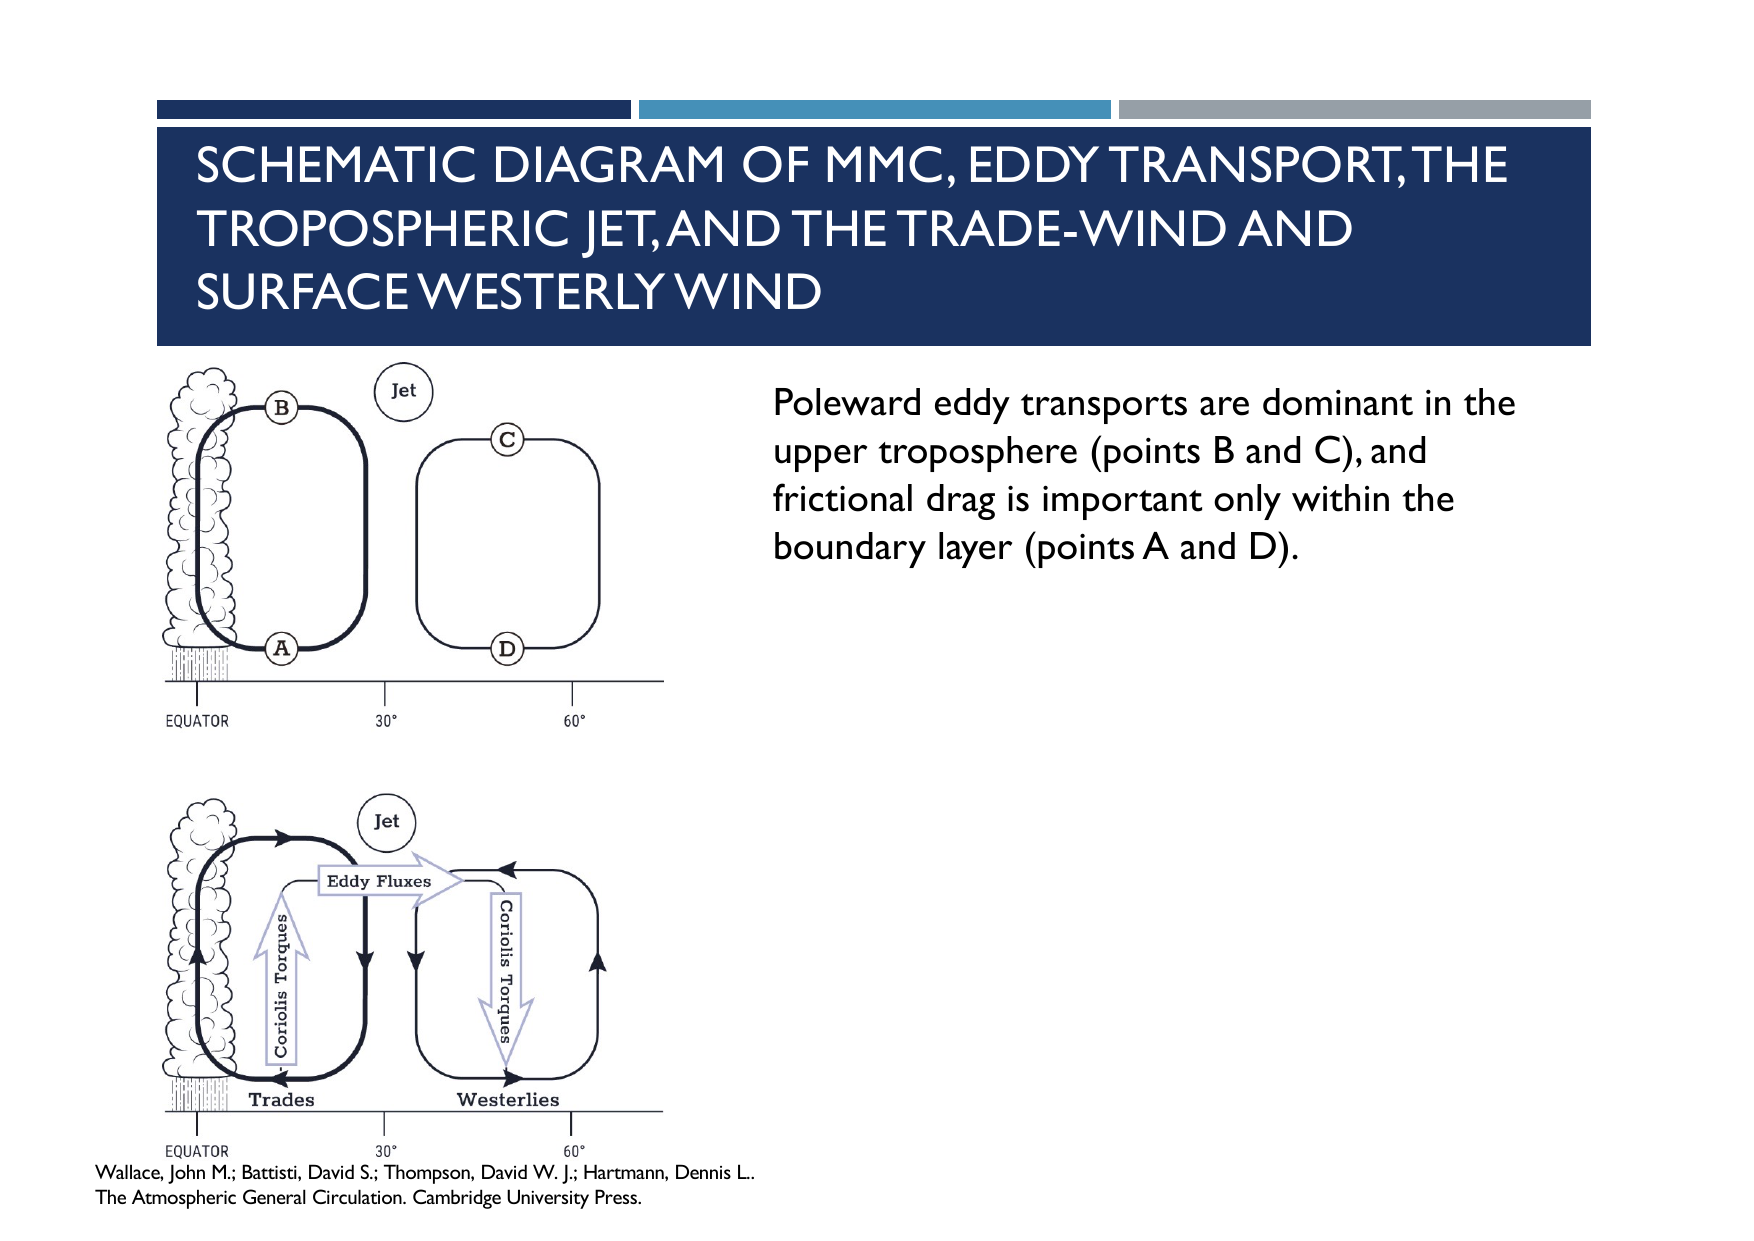
\includegraphics[width=0.85\textwidth]{images/ch07/p56_img01.png}
  \caption{Schematic synthesis of the angular momentum budget in a meridional
  cross-section: three mean meridional circulation cells (Hadley, Ferrel, Polar),
  the subtropical and polar-front jets, surface trade winds and mid-latitude
  westerlies, and poleward eddy momentum transport (curved arrows in the upper
  troposphere).  Four reference points are marked: A (equatorial surface),
  B (30$^\circ$ upper troposphere), C (60$^\circ$ upper troposphere), and
  D (30$^\circ$ surface).  The AAM balance at each point is determined by a
  different combination of Coriolis acceleration $f v_Z$, frictional drag, and
  eddy flux convergence. \hisu{대기 대순환의 4-point closure 모형:
  A, D 점은 \emph{지표}에서 friction-Coriolis 균형, B, C 점은 \emph{상층}에서
  eddy-Coriolis 균형. 이 네 점의 균형이 동시에 성립할 때만 \textbf{steady jet
  + steady trade wind}가 가능하다.}}
  \label{fig:ch07_temp_synthesis}
\end{figure}


\medskip



\noindent\textbf{Point A --- Equatorial surface (trade winds).}
적도 부근 지표에서는 평균적으로 \textgr{easterly trade wind} ($u_Z < 0$)가
관측된다.  이 평형은 다음과 같이 유지된다.  Hadley cell의 하층 가지가
적도 방향 ($v_Z < 0$ in NH lower branch)으로 흐르므로, Coriolis 가속도

\begin{equation}\label{eq:ch07_temp_pointA}
  \left.\frac{\partial u_Z}{\partial t}\right|_{\text{Cor}}
    = -f v_Z > 0 \qquad (\text{at A, NH lower Hadley})
\end{equation}

\noindent
는 \emph{westerly} 방향이다.  그러나 trade wind는 시간에 따라 거의 변하지
않으므로 ($\partial u_Z/\partial t \approx 0$), 이 westerly acceleration은
무언가에 의해 정확히 상쇄되어야 한다.  그 무언가가 바로
\textgr{surface friction}이다.

\begin{equation}\label{eq:ch07_temp_pointA_bal}
  \boxed{
    -f v_Z = -\frac{1}{\rho}\frac{\partial \tau^x}{\partial z}
    \quad\Leftrightarrow\quad
    \mathcal{T}_{\text{Cor}} = -\mathcal{T}_{\text{fric}}
    \quad(\text{at A}).
  }
\end{equation}

\hisu{Easterly trade wind는 \emph{friction이 Coriolis를 정확히 상쇄}하기 때문에
유지된다.  적도 지표에서는 위로부터 westerly momentum이 내려오지만, 지표
마찰이 그것을 같은 양만큼 earth로 돌려보낸다.  이 과정에서 atmosphere는 earth로부터
westerly AM을 \emph{얻고}, 같은 양을 mid-latitude로 흘려보내는 데 사용한다.}


\medskip



\noindent\textbf{Point D --- Mid-latitude surface (westerlies).}
30--60$^\circ$ surface에서는 평균 \textgr{westerly} ($u_Z > 0$)가 관측된다.
이 평형의 본질은 A와 \emph{거꾸로}다.  Ferrel cell의 하층 가지가 극 방향
($v_Z > 0$ in NH)으로 흐르므로, Coriolis는

\begin{equation}\label{eq:ch07_temp_pointD}
  \left.\frac{\partial u_Z}{\partial t}\right|_{\text{Cor}}
    = -f v_Z < 0 \qquad (\text{at D, NH lower Ferrel})
\end{equation}

\noindent
즉 \emph{easterly} 방향으로 가속하려 한다.  그러나 westerly를 약화시키지
않으려면 무언가가 westerly를 \textbf{공급}해야 한다.  여기서 friction은
westerly에 대해 brake이지만, Ferrel cell 자체의 Coriolis 가속 (easterly
방향)과 friction (easterly 방향) 둘 다 westerly를 깎으려 한다.

따라서 D점의 균형식은 \textbf{단순한 friction-Coriolis 균형이 아니라},
\textgr{eddy momentum flux convergence}에 의한 westerly 공급이 들어가야
완성된다.

\begin{equation}\label{eq:ch07_temp_pointD_bal}
  \boxed{
    -f v_Z - \frac{1}{\rho}\frac{\partial \tau^x}{\partial z}
    - \frac{1}{\cos^2\phi}\frac{\partial}{\partial y}
      \left[\cos^2\phi\,(u_E v_E)_Z\right] = 0
    \quad(\text{at D, full balance}).
  }
\end{equation}

물리적으로: 상층 jet 위치 (point B 부근)에서 eddy가 westerly를 수렴시키고,
그 westerly는 Ferrel cell의 \emph{하강 가지}를 따라 내려와 지표에서 친절히
$u_Z > 0$을 유지한다.  Friction은 그 westerly를 갉아먹지만, eddy 공급이
그것을 상쇄한다.

\hisu{Mid-latitude 지표 westerly = (eddy-driven jet의 surface signature)
$\leftrightarrow$ (friction에 의한 surface loss).  이 둘이 같으므로 friction
torque로 atmosphere가 earth에 AM을 돌려준다 (앞 §3의 그림 그대로).}


\medskip



\noindent\textbf{Point B --- 30$^\circ$ upper troposphere (subtropical jet, eddy divergence).}
이제 위로 올라가서 상층 30$^\circ$ 부근 (subtropical jet core)을 본다.
이곳은 평균 westerly가 30 m/s를 넘는 강한 흐름이며, 동시에 \textbf{eddy
momentum flux divergence} 구역의 가장자리 (적도 쪽)다.

Hadley cell 상층 가지가 극 방향 ($v_Z > 0$)으로 흐르므로 Coriolis는

\begin{equation}\label{eq:ch07_temp_pointB}
  \left.\frac{\partial u_Z}{\partial t}\right|_{\text{Cor}}
    = -f v_Z < 0 \qquad (\text{at B, NH upper Hadley}).
\end{equation}

잠깐, 부호가 이상하다.  Hadley cell 상층은 극 방향이고 $f > 0$이니 Coriolis는
\emph{easterly}로 가속한다.  그런데 jet은 westerly다.  이는 모순처럼 보인다.

해소: AAM 보존에서 출발하자.  적도에서 출발한 공기는 큰 $M_\Omega$를 가지고
있고, 그것을 ($u, \phi$가 변하면서) $M = M_\Omega + M_r$로 보존한다.
$\phi$가 증가하면 $\cos\phi$가 감소하고, $M_\Omega = \Omega R^2\cos^2\phi$가
줄어든다.  보존되려면 $M_r = u R\cos\phi$가 그만큼 늘어야 하므로 $u$가
증가한다.  바로 이것이 \emph{Hadley cell 상층 가지가 westerly를 가져다 주는}
이유다.

다시 균형식으로 돌아오면, Hadley cell 자체는 (Coriolis 관점에서) easterly로
밀지만, AAM 보존 입장에서는 동시에 (advection으로) westerly를 가져다 준다.
\emph{고립된 (eddy-free)} Hadley cell 모형에서는 두 효과가 정확히 상쇄되어
상층은 angular-momentum conserving wind가 된다 (Held \& Hou, 1980).

그러나 실제 대기에서는 상층 westerly가 angular-momentum conserving 값보다
훨씬 \emph{작다}.  그 이유는 \textbf{eddy momentum flux divergence}가
westerly를 가져가버리기 때문이다.

\begin{equation}\label{eq:ch07_temp_pointB_bal}
  \boxed{
    \underbrace{-f v_Z}_{\text{Coriolis (east)}}
    + \underbrace{\text{advective westerly supply}}_{\text{from AM conservation}}
    + \underbrace{\frac{-1}{\cos^2\phi}\frac{\partial}{\partial y}
      [\cos^2\phi(u_E v_E)_Z]}_{\text{eddy divergence (east)}}
    = 0 \quad (\text{at B}).
  }
\end{equation}

\hisu{B점 (subtropical jet core)에서는 Hadley cell의 westerly 공급을
\emph{eddy momentum flux divergence}가 그대로 가져간다.  바로 그 가져간
westerly가 jet stream의 mid-latitude side로 전달되어 point C에서 수렴한다.}


\medskip



\noindent\textbf{Point C --- 60$^\circ$ upper troposphere (eddy convergence, polar jet).}
B에서 eddy가 westerly를 \emph{divergent}하게 가져갔다면, C (mid-latitude 상층,
보통 폴라 jet 부근)에서는 그 westerly가 \emph{convergent}하게 수렴한다.
즉 $(u_E v_E)_Z$가 30$^\circ$에서 60$^\circ$로 가면서 감소하므로,

\begin{equation}\label{eq:ch07_temp_pointC_eddy}
  -\frac{1}{\cos^2\phi}\frac{\partial}{\partial y}
    \left[\cos^2\phi\,(u_E v_E)_Z\right] > 0 \qquad (\text{at C, eddy convergence}).
\end{equation}

\noindent
이 \emph{westerly 공급}이 무한정 jet을 가속시키지 않으려면, 정확히 같은 크기의
\emph{westerly 제거} 메커니즘이 있어야 한다.  그 메커니즘이 Ferrel cell
상층의 적도 방향 가지 ($v_Z < 0$ at high lat upper)에 의한 Coriolis 가속이다.

\begin{equation}\label{eq:ch07_temp_pointC_bal}
  \boxed{
    -f v_Z + \frac{-1}{\cos^2\phi}\frac{\partial}{\partial y}
      [\cos^2\phi(u_E v_E)_Z] = 0
    \quad\Leftrightarrow\quad
    \text{Coriolis (east)} = \text{eddy convergence (west)}
    \quad(\text{at C}).
  }
\end{equation}

\hisu{C점 (폴라 jet 부근 상층)에서는 \emph{eddy가 westerly를 가져오는 속도}와
\emph{Coriolis가 westerly를 빼앗는 속도}가 정확히 같다 --- 그래서 jet은 가속도
감속도 되지 않고 steady하다.  Ferrel cell이 "thermally indirect"라는 표현은
이 사실의 다른 표현이다 (cold air rising at high lat, warm air sinking at
30$^\circ$).}


\begin{remark}[The Hadley/Ferrel boundary at $\sim 30^\circ$]
지표에서 trade wind (easterly)와 mid-latitude westerly의 경계는 정확히 30$^\circ$
부근이다.  이는 \emph{우연이 아니다}.  Hadley cell이 angular-momentum
conserving streamline을 따라 상층으로 westerly를 운반할 수 있는 가장 먼 지점
($u\to\infty$가 되기 직전)이 이 위도이며, 동시에 baroclinic instability가
강하게 일어나는 위도이다 (Held \& Hou, 1980; Lindzen \& Hou, 1988).  그
지점에서 eddy가 takeover하여 westerly를 더 극쪽으로 운반한다.  지표
trade-wind belt와 mid-latitude westerly belt의 경계가 동일한 위도에 있는
까닭은 두 belt가 모두 같은 jet의 \emph{양옆}이기 때문이다.
\end{remark}


\medskip



\noindent\textbf{Putting it together.}
A--B--C--D 4점의 균형이 동시에 성립할 때, 대기는 다음의 \textbf{closed AM
loop}을 완성한다.

\begin{enumerate}
  \item Atmosphere가 적도 지표 (A)에서 friction torque로 earth로부터
    westerly AM을 \emph{얻는다}.
  \item Hadley cell 상층이 그 AM을 30$^\circ$ (B)까지 advect한다.
  \item B에서 eddy가 momentum flux divergence로 AM을 \emph{빼앗아}
    mid/high-latitude (C)로 운반한다.
  \item C에서 Ferrel cell의 적도 방향 상층 가지 Coriolis가 eddy 공급을
    \emph{받아내고}, Ferrel cell 하층 가지를 따라 그것을 D로 내려보낸다.
  \item D (mid-latitude 지표)에서 atmosphere는 그 westerly AM을 friction
    torque로 earth에 \emph{돌려준다}.
  \item Earth는 적도에서 받은 만큼 mid-latitude에서 돌려주므로 net AM 변화 없음
    (LOD 거의 일정).  Steady state.
\end{enumerate}

\hisu{이 6단계 closure가 \textbf{Ch.~7 전체의 핵심 결론}이다.  Trade wind와
mid-latitude westerly는 독립된 현상이 아니라 \emph{같은 jet의 두 발자국}이며,
그 사이를 connect하는 것이 (i) Hadley cell의 advection, (ii) eddy momentum
flux의 divergence-convergence, (iii) Ferrel cell의 thermally indirect 순환,
이 세 가지다.  $f v_Z$ 항과 eddy flux convergence 항의 부호가 위도-고도에서
어떻게 짝을 이루는지를 외우는 것이 곧 대기 대순환의 dynamic core를 외우는
것이다.}


\begin{hisublock}
\textbf{Held (2019) 책 Ch.~6의 4-point analysis와의 대조.}
Held, \textit{100 Years of Earth System Science at Princeton}, Ch.~6
(또는 그의 강의 노트 \textit{Hadley Circulation and Dynamics of the
Atmosphere})에서 동일한 4-point closure가 다른 표기로 제시되어 있다.
본 책의 A, B, C, D는 Held의 표기에서 각각 "equatorial easterly", "subtropical
jet exit", "polar jet entrance", "mid-latitude surface westerly"에 대응된다.
Held \& Hou (1980, \textit{J.\ Atmos.\ Sci.}, 37, 515--533)는 eddy-free
Hadley cell 모형으로 (i)--(ii) 단계를, Held \& Suarez (1978)는 nonlinear
baroclinic eddies로 (iii)--(iv) 단계를 정량적으로 다뤘다.  본 절의
schematic을 Held (2019) Figure 6.2와 직접 비교하면, 본 책의 schematic은
SH/NH symmetric annual mean 형태를 강조하는 반면 Held의 그림은 winter
hemisphere asymmetry를 포함한다는 차이가 있다.
\end{hisublock}


% =============================================================================
%   CHAPTER 7 SUMMARY (맺음말)
% =============================================================================

\subsection*{Chapter 7 Summary}

지금까지 Ch.~7에서 우리는 atmospheric angular momentum (AAM)의 \emph{정의 →
보존 → 수송 → 시간 변동}이라는 일관된 흐름을 따라 대기 대순환의 운동량
수지를 구축했다.  이 절은 그 전체를 압축한다.


\begin{remarkbox}
\textbf{Chapter 7 핵심 결론 (Angular Momentum Budget):}
\begin{enumerate}
  \item \textbf{AM의 분해}: $M = \Omega R^2\cos^2\phi + uR\cos\phi
    = M_\Omega + M_r$.  Solid-earth rotation 성분과 relative wind 성분으로
    분리되며, 단위질량당 비율은 위도에 따라 0--46, 전체질량 기준으로 $\sim 10^6$.
  \item \textbf{Conservation-only argument의 비현실성}: 적도 공기를 60$^\circ$로
    이동시키면 $u\approx 134$ m/s ($\Omega R\sin^2\phi/\cos\phi$)라는 비현실적
    값이 나온다.  \emph{Eddy transport}가 반드시 필요하다.
  \item \textbf{Sigma 좌표 flux form derivation}: $\sigma = p/p_s$로 산악
    boundary 문제를 우회하고, zonal mean + vertical integration 후 3-term
    zonal AAM budget이 도출된다:
    (i) meridional flux convergence, (ii) friction torque, (iii) mountain torque.
  \item \textbf{Surface torques}: long-term mean에서 friction이 압도적이며,
    mountain torque는 NH mid-latitude에서 약 50\%를 차지한다.  Gravity-wave
    drag는 별도 mechanism으로, 작은 산악에서도 vertically propagating wave를
    통해 stratosphere까지 AM을 운반한다.
  \item \textbf{Source-sink 구조}: tropics (0--30$^\circ$)는 AAM source
    (friction torque로 atmosphere가 AM을 얻음), extratropics는 AAM sink.
    이 차이를 \emph{poleward eddy momentum flux}가 메운다.
  \item \textbf{$(u_E v_E)_Z > 0$ 의 필요조건}: trough-ridge 축이 SW-NE로
    기울어진 \emph{eastward-tilted} 파동.  이 tilt가 baroclinic eddy의
    upgradient momentum transport를 가능케 한다 (ch.~4 결과와 동일).
  \item \textbf{Time variations}:
    \begin{itemize}
      \item Monthly: LOD-AAM 1:1 대응 → closed system 증거.
      \item Daily: torque-tendency 상관 $r\approx 0.86$ (Egger \& Hoinka 1999).
        $\pm 6$--$8\times 10^{-3}$ kg m$^2$ s$^{-2}$ 진폭의 강한 변동.
      \item Mountain pressure torque의 spatial pattern: 남태평양 (안데스
        풍하측)이 가장 강한 action center.
    \end{itemize}
  \item \textbf{MMC-eddy-friction의 4-point closure}: A (적도 지표, friction
    공급), B (subtropical jet, eddy divergence), C (폴라 jet, eddy convergence),
    D (mid-lat 지표, friction 회수)의 4점이 동시에 균형을 이뤄 \emph{steady}
    trade wind + steady westerly jet을 유지한다.
\end{enumerate}
\end{remarkbox}


\begin{hisublock}
\textbf{한국어 종합 정리}:
\begin{enumerate}
  \item AAM은 \emph{지구가 회전하기 때문에 생기는 부분} ($M_\Omega$)과
    \emph{바람이 솔리드 어스 회전과 다르기 때문에 생기는 부분} ($M_r$)의 합이다.
    측정 가능한 LOD 변동의 거의 100\%는 후자에서 온다.
  \item 적도 공기를 그대로 극으로 보내면 시속 약 500 km의 \emph{말도 안되는}
    westerly jet이 만들어진다.  관측은 그보다 훨씬 약하므로, eddy가 AM을
    꺼내가는 메커니즘이 \emph{필수}다.  Ch.~7 전체의 출발점.
  \item 산이 있어서 isobaric 좌표에서 계산이 안 되므로 sigma 좌표 ($\sigma = p/p_s$)
    로 옮긴다.  Zonal 평균을 취하고 연직 적분하면, AAM 변동은 (i) 위도방향
    flux convergence, (ii) 지표 마찰 토크, (iii) 산악 압력 토크의 3개로 깔끔하게
    압축된다.
  \item Long-term에선 마찰 토크가 주도하지만, 산악 토크도 NH 중위도에선 절반을
    먹는다.  Gravity wave drag는 별개의 메커니즘으로 stratosphere AM 균형에
    핵심.
  \item 적도는 westerly trade의 \emph{역설}: 표면 동풍인데 atmosphere는
    \emph{westerly AM을 얻는다}.  이는 friction이 negative $u$를 0으로 끌어올리는
    힘 = westerly 가속이기 때문.  중위도는 정반대로 westerly가 친 friction에
    의해 깎이는 곳.  그 사이를 eddy가 메운다.
  \item 위 운동량 수송은 baroclinic wave의 \emph{SW-NE 기울기}가 만든다.
    같은 ridge라도 기울지 않으면 upgradient momentum flux 0.  이 SW-NE tilt가
    Rossby wave dispersion (group velocity)과 동전의 양면.
  \item 매일의 AAM 변동을 보면 (Fig.~\ref{fig:ch07_temp_daily}), tendency와
    torque가 거의 손잡고 간다.  이는 eddy flux가 \emph{global} 적분에선 0이라는
    사실 (위도 간 transfer일 뿐 generation 아님)의 직접 증거다.
  \item 모든 그림이 모여 \emph{4점 closure}: A에서 받고, B에서 위로 올리고
    옆으로 빼앗기고, C에서 받고, D에서 돌려준다.  이 순환이 끊임없이 돌아가기에
    지구는 (i) 적도 표면에서 영구히 easterly trade를 유지하고, (ii) 중위도에서
    영구히 westerly jet을 유지하며, (iii) LOD가 거의 일정하게 유지된다.
\end{enumerate}

\medskip
\textbf{책 전체의 통합 관점 (Ch.~4 → Ch.~5 → Ch.~6 → Ch.~7)}: 본 책은 대기
대순환을 네 단계로 분해하여 다뤘다.

\textbf{Ch.~4 (Zonal Mean Dynamics)}에서는 zonal mean 운동량과 열 방정식을
세우고, eddy flux의 역할을 \emph{운동량 = upgradient, 열 = downgradient}로
분리했다.  EP flux와 TEM formulation으로 mean-eddy 상호작용의 unified
description을 완성했다.

\textbf{Ch.~5 (Quasi-geostrophic Dynamics)}에서는 baroclinic eddy의
생성-전파 메커니즘을 QG PV의 conservation으로 설명했다.  Charney \&
Stern, Rossby wave dispersion, baroclinic instability 모두 Ch.~4의
eddy flux를 \emph{어디서 어떻게} 만드는지에 대한 답이었다.

\textbf{Ch.~6 (Asymmetric Circulation)}에서는 zonal asymmetry, 즉
stationary wave를 도입하여 산악과 land-sea contrast가 어떻게 climatological
3D pattern을 만드는지를 보았다.  Storm track과 transient eddy도 이 stationary
배경 위에서 정의된다.

\textbf{Ch.~7 (Angular Momentum Budget)}는 위 모든 것을 하나의 \emph{보존
법칙} 위에 종합한다.  Eddy flux (Ch.~4), baroclinic eddy 생성 (Ch.~5),
stationary wave + mountain torque (Ch.~6), 4-point closure (Ch.~7)는 모두
같은 AM 수지의 다른 facet이다.  궁극적으로 trade wind, westerly jet, Hadley/Ferrel
cell, baroclinic storm track 모두 \textbf{differential solar heating}이라는
하나의 forcing에 대한 대기의 \emph{angular-momentum-conserving} 응답이다.

이 통합 관점은 향후 더 advanced한 주제 --- annular mode (NAM/SAM), QBO,
ENSO와 AM의 관계, climate change 하의 jet shift, eddy-driven jet의 internal
variability --- 를 다룰 때 출발점이 된다.  Wallace, Battisti, Thompson,
Hartmann (2023, \textit{The Atmospheric General Circulation}, Cambridge UP)는
이 관점을 가장 체계적으로 정리한 최신 참고문헌이다.
\end{hisublock}


\begin{hisublock}
\textbf{참고 문헌 가이드 (Ch.~7 전체):}
\begin{itemize}
  \item Peixoto \& Oort (1992), \textit{Physics of Climate}, Ch.~11 (pp.~275--313)
    --- AAM의 \emph{관측 표준 참고문헌}.  Hemispheric/global AM budget table
    (Table~11.1), LOD-AAM correspondence, seasonal cycle, eddy flux 모두 포함.
  \item Holton \& Hakim (2012), \textit{An Introduction to Dynamic Meteorology}
    (5th ed.), Ch.~10.3 --- mean meridional circulation과 EP flux를 통한 AM
    budget의 통합 기술. 본 책 Ch.~4 TEM 결과를 Ch.~7 budget에 직접 적용하는
    bridge.
  \item Rosen \& Salstein (1983, \textit{J.\ Geophys.\ Res.}, 88, 5451--5470);
    Rosen et al. (1990, ibid.\ 95, 265--275) --- LOD-AAM correspondence의
    원논문.  본 책 Fig.~\ref{fig:ch07_temp_monthly_lod_aam}의 monthly time
    series 분석 방법론을 정립.
  \item Egger \& Hoinka (1999, \textit{J.\ Atmos.\ Sci.}, 56, 1305--1313)
    --- daily torque-tendency balance의 reanalysis 검증 ($r\approx 0.86$).
    본 책 Fig.~\ref{fig:ch07_temp_daily}의 분석 방법론.
  \item Held \& Hou (1980, \textit{J.\ Atmos.\ Sci.}, 37, 515--533)
    --- nearly-inviscid Hadley cell의 angular-momentum conserving 해.
    A--B 단계의 정량 모형.
  \item Wallace, Battisti, Thompson, Hartmann (2023), \textit{The Atmospheric
    General Circulation}, Cambridge UP, Ch.~4 (AM Budget) --- 본 책 Ch.~7의
    구조가 가장 가까운 modern reference.
  \item Lorenz (1967, WMO No.218) --- \textit{The Nature and Theory of the
    General Circulation of the Atmosphere}, classic monograph로 본 4-point
    closure의 origin.
\end{itemize}
\end{hisublock}


\vspace{6pt}
\noindent\textit{References:
Peixoto \& Oort, \textit{Physics of Climate}, Ch.~11;
Wallace, Battisti, Thompson, and Hartmann, \textit{The Atmospheric General
Circulation}, Cambridge University Press, Ch.~4;
Holton and Hakim, \textit{An Introduction to Dynamic Meteorology},
Ch.~10.3;
Rosen \& Salstein (1983); Egger \& Hoinka (1999); Held \& Hou (1980).}
